\documentclass[10pt,a4paper]{article}
\usepackage[T1]{fontenc}
\usepackage[utf8]{inputenc}
\usepackage{mathpazo}
\usepackage[margin=20mm]{geometry}
\usepackage{microtype,graphicx,booktabs,array,tabularx,amsmath,amssymb}
\usepackage[numbers,sort&compress]{natbib}
\usepackage{xcolor,caption,placeins,fancyhdr,hyperref}
\hypersetup{colorlinks=true,linkcolor=blue!45!black,citecolor=blue!45!black,urlcolor=blue!45!black,
pdftitle={Task-Contract-Aware Online Inverse Kinematics: Aligning Solver Convergence with Command Admissibility}}
\captionsetup{font=small,labelfont=bf}
\graphicspath{{figures/}}
% Generated from frozen evidence; do not edit.
\expandafter\def\csname ev@allocation.panda.full_geometry.fev_ratio\endcsname{1.001 [1.000, 1.001]}
\expandafter\def\csname ev@allocation.panda.full_geometry.fev_reduction_pct\endcsname{-0.05}
\expandafter\def\csname ev@allocation.panda.full_geometry.latency_ratio\endcsname{1.001 [1.000, 1.002]}
\expandafter\def\csname ev@allocation.panda.full_geometry.p95_ratio\endcsname{1.002 [0.992, 1.039]}
\expandafter\def\csname ev@allocation.panda.full_geometry.p99_ratio\endcsname{1.000 [0.999, 1.002]}
\expandafter\def\csname ev@allocation.panda.full_geometry.time_increase_pct\endcsname{0.09}
\expandafter\def\csname ev@allocation.panda.full_hard.fev_ratio\endcsname{1.001 [1.001, 1.002]}
\expandafter\def\csname ev@allocation.panda.full_hard.fev_reduction_pct\endcsname{-0.12}
\expandafter\def\csname ev@allocation.panda.full_hard.latency_ratio\endcsname{1.033 [1.029, 1.038]}
\expandafter\def\csname ev@allocation.panda.full_hard.p95_ratio\endcsname{1.007 [1.002, 1.061]}
\expandafter\def\csname ev@allocation.panda.full_hard.p99_ratio\endcsname{1.001 [1.000, 1.004]}
\expandafter\def\csname ev@allocation.panda.full_hard.time_increase_pct\endcsname{3.33}
\expandafter\def\csname ev@allocation.panda.joint_failure_share\endcsname{99.07}
\expandafter\def\csname ev@allocation.panda.p95_p50.fev_ratio\endcsname{0.994 [0.992, 0.996]}
\expandafter\def\csname ev@allocation.panda.p95_p50.fev_reduction_pct\endcsname{0.58}
\expandafter\def\csname ev@allocation.panda.p95_p50.latency_ratio\endcsname{0.998 [0.997, 1.000]}
\expandafter\def\csname ev@allocation.panda.p95_p50.p95_ratio\endcsname{0.997 [0.976, 1.010]}
\expandafter\def\csname ev@allocation.panda.p95_p50.p99_ratio\endcsname{1.000 [0.998, 1.002]}
\expandafter\def\csname ev@allocation.panda.p95_p50.time_increase_pct\endcsname{-0.15}
\expandafter\def\csname ev@allocation.panda.routing_hard.fev_ratio\endcsname{1.001 [1.001, 1.002]}
\expandafter\def\csname ev@allocation.panda.routing_hard.fev_reduction_pct\endcsname{-0.12}
\expandafter\def\csname ev@allocation.panda.routing_hard.latency_ratio\endcsname{1.033 [1.030, 1.038]}
\expandafter\def\csname ev@allocation.panda.routing_hard.time_increase_pct\endcsname{3.34}
\expandafter\def\csname ev@allocation.ur5e.full_geometry.fev_ratio\endcsname{0.999 [0.996, 1.000]}
\expandafter\def\csname ev@allocation.ur5e.full_geometry.fev_reduction_pct\endcsname{0.14}
\expandafter\def\csname ev@allocation.ur5e.full_geometry.latency_ratio\endcsname{1.002 [0.998, 1.005]}
\expandafter\def\csname ev@allocation.ur5e.full_geometry.p95_ratio\endcsname{0.997 [0.973, 1.017]}
\expandafter\def\csname ev@allocation.ur5e.full_geometry.p99_ratio\endcsname{0.898 [0.775, 1.034]}
\expandafter\def\csname ev@allocation.ur5e.full_geometry.time_increase_pct\endcsname{0.17}
\expandafter\def\csname ev@allocation.ur5e.full_hard.fev_ratio\endcsname{1.000 [1.000, 1.001]}
\expandafter\def\csname ev@allocation.ur5e.full_hard.fev_reduction_pct\endcsname{-0.05}
\expandafter\def\csname ev@allocation.ur5e.full_hard.latency_ratio\endcsname{1.293 [1.286, 1.300]}
\expandafter\def\csname ev@allocation.ur5e.full_hard.p95_ratio\endcsname{1.227 [1.188, 1.261]}
\expandafter\def\csname ev@allocation.ur5e.full_hard.p99_ratio\endcsname{1.096 [1.006, 1.162]}
\expandafter\def\csname ev@allocation.ur5e.full_hard.time_increase_pct\endcsname{29.32}
\expandafter\def\csname ev@allocation.ur5e.joint_failure_share\endcsname{101.31}
\expandafter\def\csname ev@allocation.ur5e.p95_p50.fev_ratio\endcsname{0.981 [0.974, 0.989]}
\expandafter\def\csname ev@allocation.ur5e.p95_p50.fev_reduction_pct\endcsname{1.86}
\expandafter\def\csname ev@allocation.ur5e.p95_p50.latency_ratio\endcsname{0.998 [0.994, 1.002]}
\expandafter\def\csname ev@allocation.ur5e.p95_p50.p95_ratio\endcsname{0.989 [0.962, 1.010]}
\expandafter\def\csname ev@allocation.ur5e.p95_p50.p99_ratio\endcsname{0.937 [0.864, 1.053]}
\expandafter\def\csname ev@allocation.ur5e.p95_p50.time_increase_pct\endcsname{-0.17}
\expandafter\def\csname ev@allocation.ur5e.routing_hard.fev_ratio\endcsname{1.000 [1.000, 1.001]}
\expandafter\def\csname ev@allocation.ur5e.routing_hard.fev_reduction_pct\endcsname{-0.05}
\expandafter\def\csname ev@allocation.ur5e.routing_hard.latency_ratio\endcsname{1.294 [1.286, 1.300]}
\expandafter\def\csname ev@allocation.ur5e.routing_hard.time_increase_pct\endcsname{29.35}
\expandafter\def\csname ev@contract.dt_ms\endcsname{20}
\expandafter\def\csname ev@contract.ep_mm\endcsname{1}
\expandafter\def\csname ev@contract.er_deg\endcsname{0.5}
\expandafter\def\csname ev@contract.ev\endcsname{0.0001}
\expandafter\def\csname ev@dls.panda.admissible_queries\endcsname{2487}
\expandafter\def\csname ev@dls.panda.median_excess_evaluations\endcsname{2}
\expandafter\def\csname ev@dls.panda.median_excess_iterations\endcsname{1}
\expandafter\def\csname ev@dls.panda.mismatch_pct\endcsname{21.92}
\expandafter\def\csname ev@dls.panda.p95_excess_evaluations\endcsname{49}
\expandafter\def\csname ev@dls.panda.p95_excess_iterations\endcsname{24}
\expandafter\def\csname ev@dls.panda.positive_excess_queries\endcsname{2397}
\expandafter\def\csname ev@dls.ur5e.admissible_queries\endcsname{2499}
\expandafter\def\csname ev@dls.ur5e.median_excess_evaluations\endcsname{2}
\expandafter\def\csname ev@dls.ur5e.median_excess_iterations\endcsname{1}
\expandafter\def\csname ev@dls.ur5e.mismatch_pct\endcsname{21.24}
\expandafter\def\csname ev@dls.ur5e.p95_excess_evaluations\endcsname{49}
\expandafter\def\csname ev@dls.ur5e.p95_excess_iterations\endcsname{24}
\expandafter\def\csname ev@dls.ur5e.positive_excess_queries\endcsname{2346}
\expandafter\def\csname ev@family.panda.high_curvature.gained\endcsname{0}
\expandafter\def\csname ev@family.panda.joint_limit_return.gained\endcsname{0}
\expandafter\def\csname ev@family.panda.near_singular.gained\endcsname{3}
\expandafter\def\csname ev@family.panda.smooth.gained\endcsname{0}
\expandafter\def\csname ev@family.ur5e.high_curvature.gained\endcsname{1}
\expandafter\def\csname ev@family.ur5e.joint_limit_return.gained\endcsname{0}
\expandafter\def\csname ev@family.ur5e.near_singular.gained\endcsname{0}
\expandafter\def\csname ev@family.ur5e.smooth.gained\endcsname{1}
\expandafter\def\csname ev@point.panda.dls_strict.accepted_within_20ms\endcsname{99.48}
\expandafter\def\csname ev@point.panda.dls_strict.contrast.gained\endcsname{0}
\expandafter\def\csname ev@point.panda.dls_strict.contrast.lost\endcsname{13}
\expandafter\def\csname ev@point.panda.dls_strict.contrast.saving_pct\endcsname{-1175.58}
\expandafter\def\csname ev@point.panda.dls_strict.contrast.success_pp\endcsname{-0.520 [-0.840, -0.280]}
\expandafter\def\csname ev@point.panda.dls_strict.contrast.time_ratio\endcsname{12.756 [12.313, 13.187]}
\expandafter\def\csname ev@point.panda.dls_strict.internal_failure__task_accept\endcsname{548}
\expandafter\def\csname ev@point.panda.dls_strict.internal_failure__task_reject\endcsname{13}
\expandafter\def\csname ev@point.panda.dls_strict.internal_success\endcsname{77.56}
\expandafter\def\csname ev@point.panda.dls_strict.internal_success__task_accept\endcsname{1939}
\expandafter\def\csname ev@point.panda.dls_strict.internal_success__task_reject\endcsname{0}
\expandafter\def\csname ev@point.panda.dls_strict.mean\endcsname{3.015}
\expandafter\def\csname ev@point.panda.dls_strict.miss_uid\endcsname{13}
\expandafter\def\csname ev@point.panda.dls_strict.orientation_max\endcsname{0.2378}
\expandafter\def\csname ev@point.panda.dls_strict.orientation_p50\endcsname{0.0001}
\expandafter\def\csname ev@point.panda.dls_strict.orientation_p95\endcsname{0.0036}
\expandafter\def\csname ev@point.panda.dls_strict.orientation_p99\endcsname{0.0474}
\expandafter\def\csname ev@point.panda.dls_strict.p50\endcsname{1.038}
\expandafter\def\csname ev@point.panda.dls_strict.p95\endcsname{8.944}
\expandafter\def\csname ev@point.panda.dls_strict.p99\endcsname{9.230}
\expandafter\def\csname ev@point.panda.dls_strict.position_max\endcsname{0.8801}
\expandafter\def\csname ev@point.panda.dls_strict.position_p50\endcsname{0.0007}
\expandafter\def\csname ev@point.panda.dls_strict.position_p95\endcsname{0.0572}
\expandafter\def\csname ev@point.panda.dls_strict.position_p99\endcsname{0.2693}
\expandafter\def\csname ev@point.panda.dls_strict.verified_success\endcsname{99.48}
\expandafter\def\csname ev@point.panda.dls_task.accepted_within_20ms\endcsname{99.48}
\expandafter\def\csname ev@point.panda.dls_task.contrast.gained\endcsname{0}
\expandafter\def\csname ev@point.panda.dls_task.contrast.lost\endcsname{0}
\expandafter\def\csname ev@point.panda.dls_task.contrast.saving_pct\endcsname{74.72}
\expandafter\def\csname ev@point.panda.dls_task.contrast.success_pp\endcsname{0.000 [0.000, 0.000]}
\expandafter\def\csname ev@point.panda.dls_task.contrast.time_ratio\endcsname{0.253 [0.243, 0.264]}
\expandafter\def\csname ev@point.panda.dls_task.internal_failure__task_accept\endcsname{0}
\expandafter\def\csname ev@point.panda.dls_task.internal_failure__task_reject\endcsname{13}
\expandafter\def\csname ev@point.panda.dls_task.internal_success\endcsname{99.48}
\expandafter\def\csname ev@point.panda.dls_task.internal_success__task_accept\endcsname{2487}
\expandafter\def\csname ev@point.panda.dls_task.internal_success__task_reject\endcsname{0}
\expandafter\def\csname ev@point.panda.dls_task.mean\endcsname{0.762}
\expandafter\def\csname ev@point.panda.dls_task.miss_uid\endcsname{13}
\expandafter\def\csname ev@point.panda.dls_task.orientation_max\endcsname{0.4988}
\expandafter\def\csname ev@point.panda.dls_task.orientation_p50\endcsname{0.0154}
\expandafter\def\csname ev@point.panda.dls_task.orientation_p95\endcsname{0.1447}
\expandafter\def\csname ev@point.panda.dls_task.orientation_p99\endcsname{0.3157}
\expandafter\def\csname ev@point.panda.dls_task.p50\endcsname{0.625}
\expandafter\def\csname ev@point.panda.dls_task.p95\endcsname{1.042}
\expandafter\def\csname ev@point.panda.dls_task.p99\endcsname{4.479}
\expandafter\def\csname ev@point.panda.dls_task.position_max\endcsname{0.9958}
\expandafter\def\csname ev@point.panda.dls_task.position_p50\endcsname{0.1126}
\expandafter\def\csname ev@point.panda.dls_task.position_p95\endcsname{0.8004}
\expandafter\def\csname ev@point.panda.dls_task.position_p99\endcsname{0.9639}
\expandafter\def\csname ev@point.panda.dls_task.verified_success\endcsname{99.48}
\expandafter\def\csname ev@point.panda.trac_orientation_5ms.accepted_within_20ms\endcsname{100.00}
\expandafter\def\csname ev@point.panda.trac_orientation_5ms.contrast.gained\endcsname{0}
\expandafter\def\csname ev@point.panda.trac_orientation_5ms.contrast.lost\endcsname{0}
\expandafter\def\csname ev@point.panda.trac_orientation_5ms.contrast.saving_pct\endcsname{-4.30}
\expandafter\def\csname ev@point.panda.trac_orientation_5ms.contrast.success_pp\endcsname{0.000 [0.000, 0.000]}
\expandafter\def\csname ev@point.panda.trac_orientation_5ms.contrast.time_ratio\endcsname{1.043 [1.025, 1.064]}
\expandafter\def\csname ev@point.panda.trac_orientation_5ms.internal_failure__task_accept\endcsname{0}
\expandafter\def\csname ev@point.panda.trac_orientation_5ms.internal_failure__task_reject\endcsname{0}
\expandafter\def\csname ev@point.panda.trac_orientation_5ms.internal_success\endcsname{100.00}
\expandafter\def\csname ev@point.panda.trac_orientation_5ms.internal_success__task_accept\endcsname{7500}
\expandafter\def\csname ev@point.panda.trac_orientation_5ms.internal_success__task_reject\endcsname{0}
\expandafter\def\csname ev@point.panda.trac_orientation_5ms.mean\endcsname{0.247}
\expandafter\def\csname ev@point.panda.trac_orientation_5ms.miss_uid\endcsname{0}
\expandafter\def\csname ev@point.panda.trac_orientation_5ms.orientation_max\endcsname{0.3762}
\expandafter\def\csname ev@point.panda.trac_orientation_5ms.orientation_p50\endcsname{0.0000}
\expandafter\def\csname ev@point.panda.trac_orientation_5ms.orientation_p95\endcsname{0.0031}
\expandafter\def\csname ev@point.panda.trac_orientation_5ms.orientation_p99\endcsname{0.2667}
\expandafter\def\csname ev@point.panda.trac_orientation_5ms.p50\endcsname{0.210}
\expandafter\def\csname ev@point.panda.trac_orientation_5ms.p95\endcsname{0.382}
\expandafter\def\csname ev@point.panda.trac_orientation_5ms.p99\endcsname{0.799}
\expandafter\def\csname ev@point.panda.trac_orientation_5ms.position_max\endcsname{0.0157}
\expandafter\def\csname ev@point.panda.trac_orientation_5ms.position_p50\endcsname{0.0003}
\expandafter\def\csname ev@point.panda.trac_orientation_5ms.position_p95\endcsname{0.0103}
\expandafter\def\csname ev@point.panda.trac_orientation_5ms.position_p99\endcsname{0.0129}
\expandafter\def\csname ev@point.panda.trac_orientation_5ms.verified_success\endcsname{100.00}
\expandafter\def\csname ev@point.panda.trac_position_5ms.accepted_within_20ms\endcsname{100.00}
\expandafter\def\csname ev@point.panda.trac_position_5ms.contrast.gained\endcsname{0}
\expandafter\def\csname ev@point.panda.trac_position_5ms.contrast.lost\endcsname{0}
\expandafter\def\csname ev@point.panda.trac_position_5ms.contrast.saving_pct\endcsname{-2.16}
\expandafter\def\csname ev@point.panda.trac_position_5ms.contrast.success_pp\endcsname{0.000 [0.000, 0.000]}
\expandafter\def\csname ev@point.panda.trac_position_5ms.contrast.time_ratio\endcsname{1.022 [1.011, 1.032]}
\expandafter\def\csname ev@point.panda.trac_position_5ms.internal_failure__task_accept\endcsname{0}
\expandafter\def\csname ev@point.panda.trac_position_5ms.internal_failure__task_reject\endcsname{0}
\expandafter\def\csname ev@point.panda.trac_position_5ms.internal_success\endcsname{100.00}
\expandafter\def\csname ev@point.panda.trac_position_5ms.internal_success__task_accept\endcsname{7500}
\expandafter\def\csname ev@point.panda.trac_position_5ms.internal_success__task_reject\endcsname{0}
\expandafter\def\csname ev@point.panda.trac_position_5ms.mean\endcsname{0.241}
\expandafter\def\csname ev@point.panda.trac_position_5ms.miss_uid\endcsname{0}
\expandafter\def\csname ev@point.panda.trac_position_5ms.orientation_max\endcsname{0.0009}
\expandafter\def\csname ev@point.panda.trac_position_5ms.orientation_p50\endcsname{0.0000}
\expandafter\def\csname ev@point.panda.trac_position_5ms.orientation_p95\endcsname{0.0005}
\expandafter\def\csname ev@point.panda.trac_position_5ms.orientation_p99\endcsname{0.0007}
\expandafter\def\csname ev@point.panda.trac_position_5ms.p50\endcsname{0.211}
\expandafter\def\csname ev@point.panda.trac_position_5ms.p95\endcsname{0.379}
\expandafter\def\csname ev@point.panda.trac_position_5ms.p99\endcsname{0.681}
\expandafter\def\csname ev@point.panda.trac_position_5ms.position_max\endcsname{0.9651}
\expandafter\def\csname ev@point.panda.trac_position_5ms.position_p50\endcsname{0.0001}
\expandafter\def\csname ev@point.panda.trac_position_5ms.position_p95\endcsname{0.4487}
\expandafter\def\csname ev@point.panda.trac_position_5ms.position_p99\endcsname{0.7651}
\expandafter\def\csname ev@point.panda.trac_position_5ms.verified_success\endcsname{100.00}
\expandafter\def\csname ev@point.panda.trac_strict_20ms.accepted_within_20ms\endcsname{100.00}
\expandafter\def\csname ev@point.panda.trac_strict_20ms.contrast.gained\endcsname{0}
\expandafter\def\csname ev@point.panda.trac_strict_20ms.contrast.lost\endcsname{0}
\expandafter\def\csname ev@point.panda.trac_strict_20ms.contrast.saving_pct\endcsname{0.27}
\expandafter\def\csname ev@point.panda.trac_strict_20ms.contrast.success_pp\endcsname{0.000 [0.000, 0.000]}
\expandafter\def\csname ev@point.panda.trac_strict_20ms.contrast.time_ratio\endcsname{0.997 [0.993, 1.002]}
\expandafter\def\csname ev@point.panda.trac_strict_20ms.internal_failure__task_accept\endcsname{0}
\expandafter\def\csname ev@point.panda.trac_strict_20ms.internal_failure__task_reject\endcsname{0}
\expandafter\def\csname ev@point.panda.trac_strict_20ms.internal_success\endcsname{100.00}
\expandafter\def\csname ev@point.panda.trac_strict_20ms.internal_success__task_accept\endcsname{7500}
\expandafter\def\csname ev@point.panda.trac_strict_20ms.internal_success__task_reject\endcsname{0}
\expandafter\def\csname ev@point.panda.trac_strict_20ms.mean\endcsname{0.236}
\expandafter\def\csname ev@point.panda.trac_strict_20ms.miss_uid\endcsname{0}
\expandafter\def\csname ev@point.panda.trac_strict_20ms.orientation_max\endcsname{0.0009}
\expandafter\def\csname ev@point.panda.trac_strict_20ms.orientation_p50\endcsname{0.0000}
\expandafter\def\csname ev@point.panda.trac_strict_20ms.orientation_p95\endcsname{0.0005}
\expandafter\def\csname ev@point.panda.trac_strict_20ms.orientation_p99\endcsname{0.0007}
\expandafter\def\csname ev@point.panda.trac_strict_20ms.p50\endcsname{0.211}
\expandafter\def\csname ev@point.panda.trac_strict_20ms.p95\endcsname{0.362}
\expandafter\def\csname ev@point.panda.trac_strict_20ms.p99\endcsname{0.485}
\expandafter\def\csname ev@point.panda.trac_strict_20ms.position_max\endcsname{0.0161}
\expandafter\def\csname ev@point.panda.trac_strict_20ms.position_p50\endcsname{0.0001}
\expandafter\def\csname ev@point.panda.trac_strict_20ms.position_p95\endcsname{0.0073}
\expandafter\def\csname ev@point.panda.trac_strict_20ms.position_p99\endcsname{0.0109}
\expandafter\def\csname ev@point.panda.trac_strict_20ms.verified_success\endcsname{100.00}
\expandafter\def\csname ev@point.panda.trac_strict_5ms.accepted_within_20ms\endcsname{100.00}
\expandafter\def\csname ev@point.panda.trac_strict_5ms.internal_failure__task_accept\endcsname{0}
\expandafter\def\csname ev@point.panda.trac_strict_5ms.internal_failure__task_reject\endcsname{0}
\expandafter\def\csname ev@point.panda.trac_strict_5ms.internal_success\endcsname{100.00}
\expandafter\def\csname ev@point.panda.trac_strict_5ms.internal_success__task_accept\endcsname{7500}
\expandafter\def\csname ev@point.panda.trac_strict_5ms.internal_success__task_reject\endcsname{0}
\expandafter\def\csname ev@point.panda.trac_strict_5ms.mean\endcsname{0.236}
\expandafter\def\csname ev@point.panda.trac_strict_5ms.miss_uid\endcsname{0}
\expandafter\def\csname ev@point.panda.trac_strict_5ms.orientation_max\endcsname{0.0009}
\expandafter\def\csname ev@point.panda.trac_strict_5ms.orientation_p50\endcsname{0.0000}
\expandafter\def\csname ev@point.panda.trac_strict_5ms.orientation_p95\endcsname{0.0005}
\expandafter\def\csname ev@point.panda.trac_strict_5ms.orientation_p99\endcsname{0.0007}
\expandafter\def\csname ev@point.panda.trac_strict_5ms.p50\endcsname{0.211}
\expandafter\def\csname ev@point.panda.trac_strict_5ms.p95\endcsname{0.367}
\expandafter\def\csname ev@point.panda.trac_strict_5ms.p99\endcsname{0.487}
\expandafter\def\csname ev@point.panda.trac_strict_5ms.position_max\endcsname{0.0153}
\expandafter\def\csname ev@point.panda.trac_strict_5ms.position_p50\endcsname{0.0001}
\expandafter\def\csname ev@point.panda.trac_strict_5ms.position_p95\endcsname{0.0073}
\expandafter\def\csname ev@point.panda.trac_strict_5ms.position_p99\endcsname{0.0109}
\expandafter\def\csname ev@point.panda.trac_strict_5ms.verified_success\endcsname{100.00}
\expandafter\def\csname ev@point.panda.trac_task_20ms.accepted_within_20ms\endcsname{100.00}
\expandafter\def\csname ev@point.panda.trac_task_20ms.contrast.gained\endcsname{0}
\expandafter\def\csname ev@point.panda.trac_task_20ms.contrast.lost\endcsname{0}
\expandafter\def\csname ev@point.panda.trac_task_20ms.contrast.saving_pct\endcsname{6.46}
\expandafter\def\csname ev@point.panda.trac_task_20ms.contrast.success_pp\endcsname{0.000 [0.000, 0.000]}
\expandafter\def\csname ev@point.panda.trac_task_20ms.contrast.time_ratio\endcsname{0.935 [0.928, 0.943]}
\expandafter\def\csname ev@point.panda.trac_task_20ms.internal_failure__task_accept\endcsname{0}
\expandafter\def\csname ev@point.panda.trac_task_20ms.internal_failure__task_reject\endcsname{0}
\expandafter\def\csname ev@point.panda.trac_task_20ms.internal_success\endcsname{100.00}
\expandafter\def\csname ev@point.panda.trac_task_20ms.internal_success__task_accept\endcsname{7500}
\expandafter\def\csname ev@point.panda.trac_task_20ms.internal_success__task_reject\endcsname{0}
\expandafter\def\csname ev@point.panda.trac_task_20ms.mean\endcsname{0.220}
\expandafter\def\csname ev@point.panda.trac_task_20ms.miss_uid\endcsname{0}
\expandafter\def\csname ev@point.panda.trac_task_20ms.orientation_max\endcsname{0.4432}
\expandafter\def\csname ev@point.panda.trac_task_20ms.orientation_p50\endcsname{0.0064}
\expandafter\def\csname ev@point.panda.trac_task_20ms.orientation_p95\endcsname{0.1397}
\expandafter\def\csname ev@point.panda.trac_task_20ms.orientation_p99\endcsname{0.2884}
\expandafter\def\csname ev@point.panda.trac_task_20ms.p50\endcsname{0.199}
\expandafter\def\csname ev@point.panda.trac_task_20ms.p95\endcsname{0.331}
\expandafter\def\csname ev@point.panda.trac_task_20ms.p99\endcsname{0.467}
\expandafter\def\csname ev@point.panda.trac_task_20ms.position_max\endcsname{0.9834}
\expandafter\def\csname ev@point.panda.trac_task_20ms.position_p50\endcsname{0.0675}
\expandafter\def\csname ev@point.panda.trac_task_20ms.position_p95\endcsname{0.5698}
\expandafter\def\csname ev@point.panda.trac_task_20ms.position_p99\endcsname{0.7403}
\expandafter\def\csname ev@point.panda.trac_task_20ms.verified_success\endcsname{100.00}
\expandafter\def\csname ev@point.panda.trac_task_5ms.accepted_within_20ms\endcsname{100.00}
\expandafter\def\csname ev@point.panda.trac_task_5ms.contrast.gained\endcsname{0}
\expandafter\def\csname ev@point.panda.trac_task_5ms.contrast.lost\endcsname{0}
\expandafter\def\csname ev@point.panda.trac_task_5ms.contrast.saving_pct\endcsname{6.41}
\expandafter\def\csname ev@point.panda.trac_task_5ms.contrast.success_pp\endcsname{0.000 [0.000, 0.000]}
\expandafter\def\csname ev@point.panda.trac_task_5ms.contrast.time_ratio\endcsname{0.936 [0.928, 0.945]}
\expandafter\def\csname ev@point.panda.trac_task_5ms.internal_failure__task_accept\endcsname{0}
\expandafter\def\csname ev@point.panda.trac_task_5ms.internal_failure__task_reject\endcsname{0}
\expandafter\def\csname ev@point.panda.trac_task_5ms.internal_success\endcsname{100.00}
\expandafter\def\csname ev@point.panda.trac_task_5ms.internal_success__task_accept\endcsname{7500}
\expandafter\def\csname ev@point.panda.trac_task_5ms.internal_success__task_reject\endcsname{0}
\expandafter\def\csname ev@point.panda.trac_task_5ms.mean\endcsname{0.221}
\expandafter\def\csname ev@point.panda.trac_task_5ms.miss_uid\endcsname{0}
\expandafter\def\csname ev@point.panda.trac_task_5ms.orientation_max\endcsname{0.4432}
\expandafter\def\csname ev@point.panda.trac_task_5ms.orientation_p50\endcsname{0.0065}
\expandafter\def\csname ev@point.panda.trac_task_5ms.orientation_p95\endcsname{0.1397}
\expandafter\def\csname ev@point.panda.trac_task_5ms.orientation_p99\endcsname{0.2884}
\expandafter\def\csname ev@point.panda.trac_task_5ms.p50\endcsname{0.199}
\expandafter\def\csname ev@point.panda.trac_task_5ms.p95\endcsname{0.332}
\expandafter\def\csname ev@point.panda.trac_task_5ms.p99\endcsname{0.478}
\expandafter\def\csname ev@point.panda.trac_task_5ms.position_max\endcsname{0.8799}
\expandafter\def\csname ev@point.panda.trac_task_5ms.position_p50\endcsname{0.0678}
\expandafter\def\csname ev@point.panda.trac_task_5ms.position_p95\endcsname{0.5760}
\expandafter\def\csname ev@point.panda.trac_task_5ms.position_p99\endcsname{0.7445}
\expandafter\def\csname ev@point.panda.trac_task_5ms.verified_success\endcsname{100.00}
\expandafter\def\csname ev@point.ur5e.dls_strict.accepted_within_20ms\endcsname{99.92}
\expandafter\def\csname ev@point.ur5e.dls_strict.contrast.gained\endcsname{0}
\expandafter\def\csname ev@point.ur5e.dls_strict.contrast.lost\endcsname{1}
\expandafter\def\csname ev@point.ur5e.dls_strict.contrast.saving_pct\endcsname{-1164.64}
\expandafter\def\csname ev@point.ur5e.dls_strict.contrast.success_pp\endcsname{-0.040 [-0.120, 0.000]}
\expandafter\def\csname ev@point.ur5e.dls_strict.contrast.time_ratio\endcsname{12.646 [12.173, 13.119]}
\expandafter\def\csname ev@point.ur5e.dls_strict.internal_failure__task_accept\endcsname{531}
\expandafter\def\csname ev@point.ur5e.dls_strict.internal_failure__task_reject\endcsname{1}
\expandafter\def\csname ev@point.ur5e.dls_strict.internal_success\endcsname{78.72}
\expandafter\def\csname ev@point.ur5e.dls_strict.internal_success__task_accept\endcsname{1968}
\expandafter\def\csname ev@point.ur5e.dls_strict.internal_success__task_reject\endcsname{0}
\expandafter\def\csname ev@point.ur5e.dls_strict.mean\endcsname{2.757}
\expandafter\def\csname ev@point.ur5e.dls_strict.miss_uid\endcsname{1}
\expandafter\def\csname ev@point.ur5e.dls_strict.orientation_max\endcsname{0.0867}
\expandafter\def\csname ev@point.ur5e.dls_strict.orientation_p50\endcsname{0.0001}
\expandafter\def\csname ev@point.ur5e.dls_strict.orientation_p95\endcsname{0.0036}
\expandafter\def\csname ev@point.ur5e.dls_strict.orientation_p99\endcsname{0.0141}
\expandafter\def\csname ev@point.ur5e.dls_strict.p50\endcsname{1.185}
\expandafter\def\csname ev@point.ur5e.dls_strict.p95\endcsname{8.113}
\expandafter\def\csname ev@point.ur5e.dls_strict.p99\endcsname{8.427}
\expandafter\def\csname ev@point.ur5e.dls_strict.position_max\endcsname{0.6873}
\expandafter\def\csname ev@point.ur5e.dls_strict.position_p50\endcsname{0.0011}
\expandafter\def\csname ev@point.ur5e.dls_strict.position_p95\endcsname{0.0595}
\expandafter\def\csname ev@point.ur5e.dls_strict.position_p99\endcsname{0.1468}
\expandafter\def\csname ev@point.ur5e.dls_strict.verified_success\endcsname{99.96}
\expandafter\def\csname ev@point.ur5e.dls_task.accepted_within_20ms\endcsname{99.96}
\expandafter\def\csname ev@point.ur5e.dls_task.contrast.gained\endcsname{0}
\expandafter\def\csname ev@point.ur5e.dls_task.contrast.lost\endcsname{0}
\expandafter\def\csname ev@point.ur5e.dls_task.contrast.saving_pct\endcsname{76.19}
\expandafter\def\csname ev@point.ur5e.dls_task.contrast.success_pp\endcsname{0.000 [0.000, 0.000]}
\expandafter\def\csname ev@point.ur5e.dls_task.contrast.time_ratio\endcsname{0.238 [0.230, 0.247]}
\expandafter\def\csname ev@point.ur5e.dls_task.internal_failure__task_accept\endcsname{0}
\expandafter\def\csname ev@point.ur5e.dls_task.internal_failure__task_reject\endcsname{1}
\expandafter\def\csname ev@point.ur5e.dls_task.internal_success\endcsname{99.96}
\expandafter\def\csname ev@point.ur5e.dls_task.internal_success__task_accept\endcsname{2499}
\expandafter\def\csname ev@point.ur5e.dls_task.internal_success__task_reject\endcsname{0}
\expandafter\def\csname ev@point.ur5e.dls_task.mean\endcsname{0.656}
\expandafter\def\csname ev@point.ur5e.dls_task.miss_uid\endcsname{1}
\expandafter\def\csname ev@point.ur5e.dls_task.orientation_max\endcsname{0.4824}
\expandafter\def\csname ev@point.ur5e.dls_task.orientation_p50\endcsname{0.0157}
\expandafter\def\csname ev@point.ur5e.dls_task.orientation_p95\endcsname{0.1315}
\expandafter\def\csname ev@point.ur5e.dls_task.orientation_p99\endcsname{0.2469}
\expandafter\def\csname ev@point.ur5e.dls_task.p50\endcsname{0.578}
\expandafter\def\csname ev@point.ur5e.dls_task.p95\endcsname{0.926}
\expandafter\def\csname ev@point.ur5e.dls_task.p99\endcsname{1.458}
\expandafter\def\csname ev@point.ur5e.dls_task.position_max\endcsname{0.9994}
\expandafter\def\csname ev@point.ur5e.dls_task.position_p50\endcsname{0.1477}
\expandafter\def\csname ev@point.ur5e.dls_task.position_p95\endcsname{0.7908}
\expandafter\def\csname ev@point.ur5e.dls_task.position_p99\endcsname{0.9406}
\expandafter\def\csname ev@point.ur5e.dls_task.verified_success\endcsname{99.96}
\expandafter\def\csname ev@point.ur5e.trac_orientation_5ms.accepted_within_20ms\endcsname{99.99}
\expandafter\def\csname ev@point.ur5e.trac_orientation_5ms.contrast.gained\endcsname{0}
\expandafter\def\csname ev@point.ur5e.trac_orientation_5ms.contrast.lost\endcsname{1}
\expandafter\def\csname ev@point.ur5e.trac_orientation_5ms.contrast.saving_pct\endcsname{-0.56}
\expandafter\def\csname ev@point.ur5e.trac_orientation_5ms.contrast.success_pp\endcsname{-0.013 [-0.040, 0.000]}
\expandafter\def\csname ev@point.ur5e.trac_orientation_5ms.contrast.time_ratio\endcsname{1.006 [0.993, 1.019]}
\expandafter\def\csname ev@point.ur5e.trac_orientation_5ms.internal_failure__task_accept\endcsname{0}
\expandafter\def\csname ev@point.ur5e.trac_orientation_5ms.internal_failure__task_reject\endcsname{1}
\expandafter\def\csname ev@point.ur5e.trac_orientation_5ms.internal_success\endcsname{99.99}
\expandafter\def\csname ev@point.ur5e.trac_orientation_5ms.internal_success__task_accept\endcsname{7499}
\expandafter\def\csname ev@point.ur5e.trac_orientation_5ms.internal_success__task_reject\endcsname{0}
\expandafter\def\csname ev@point.ur5e.trac_orientation_5ms.mean\endcsname{0.219}
\expandafter\def\csname ev@point.ur5e.trac_orientation_5ms.miss_uid\endcsname{1}
\expandafter\def\csname ev@point.ur5e.trac_orientation_5ms.orientation_max\endcsname{0.4075}
\expandafter\def\csname ev@point.ur5e.trac_orientation_5ms.orientation_p50\endcsname{0.0000}
\expandafter\def\csname ev@point.ur5e.trac_orientation_5ms.orientation_p95\endcsname{0.0018}
\expandafter\def\csname ev@point.ur5e.trac_orientation_5ms.orientation_p99\endcsname{0.1187}
\expandafter\def\csname ev@point.ur5e.trac_orientation_5ms.p50\endcsname{0.200}
\expandafter\def\csname ev@point.ur5e.trac_orientation_5ms.p95\endcsname{0.324}
\expandafter\def\csname ev@point.ur5e.trac_orientation_5ms.p99\endcsname{0.445}
\expandafter\def\csname ev@point.ur5e.trac_orientation_5ms.position_max\endcsname{0.0146}
\expandafter\def\csname ev@point.ur5e.trac_orientation_5ms.position_p50\endcsname{0.0002}
\expandafter\def\csname ev@point.ur5e.trac_orientation_5ms.position_p95\endcsname{0.0091}
\expandafter\def\csname ev@point.ur5e.trac_orientation_5ms.position_p99\endcsname{0.0121}
\expandafter\def\csname ev@point.ur5e.trac_orientation_5ms.verified_success\endcsname{99.99}
\expandafter\def\csname ev@point.ur5e.trac_position_5ms.accepted_within_20ms\endcsname{100.00}
\expandafter\def\csname ev@point.ur5e.trac_position_5ms.contrast.gained\endcsname{0}
\expandafter\def\csname ev@point.ur5e.trac_position_5ms.contrast.lost\endcsname{0}
\expandafter\def\csname ev@point.ur5e.trac_position_5ms.contrast.saving_pct\endcsname{1.06}
\expandafter\def\csname ev@point.ur5e.trac_position_5ms.contrast.success_pp\endcsname{0.000 [0.000, 0.000]}
\expandafter\def\csname ev@point.ur5e.trac_position_5ms.contrast.time_ratio\endcsname{0.989 [0.979, 0.998]}
\expandafter\def\csname ev@point.ur5e.trac_position_5ms.internal_failure__task_accept\endcsname{0}
\expandafter\def\csname ev@point.ur5e.trac_position_5ms.internal_failure__task_reject\endcsname{0}
\expandafter\def\csname ev@point.ur5e.trac_position_5ms.internal_success\endcsname{100.00}
\expandafter\def\csname ev@point.ur5e.trac_position_5ms.internal_success__task_accept\endcsname{7500}
\expandafter\def\csname ev@point.ur5e.trac_position_5ms.internal_success__task_reject\endcsname{0}
\expandafter\def\csname ev@point.ur5e.trac_position_5ms.mean\endcsname{0.216}
\expandafter\def\csname ev@point.ur5e.trac_position_5ms.miss_uid\endcsname{0}
\expandafter\def\csname ev@point.ur5e.trac_position_5ms.orientation_max\endcsname{0.0008}
\expandafter\def\csname ev@point.ur5e.trac_position_5ms.orientation_p50\endcsname{0.0000}
\expandafter\def\csname ev@point.ur5e.trac_position_5ms.orientation_p95\endcsname{0.0005}
\expandafter\def\csname ev@point.ur5e.trac_position_5ms.orientation_p99\endcsname{0.0006}
\expandafter\def\csname ev@point.ur5e.trac_position_5ms.p50\endcsname{0.199}
\expandafter\def\csname ev@point.ur5e.trac_position_5ms.p95\endcsname{0.317}
\expandafter\def\csname ev@point.ur5e.trac_position_5ms.p99\endcsname{0.414}
\expandafter\def\csname ev@point.ur5e.trac_position_5ms.position_max\endcsname{0.8589}
\expandafter\def\csname ev@point.ur5e.trac_position_5ms.position_p50\endcsname{0.0002}
\expandafter\def\csname ev@point.ur5e.trac_position_5ms.position_p95\endcsname{0.1120}
\expandafter\def\csname ev@point.ur5e.trac_position_5ms.position_p99\endcsname{0.5958}
\expandafter\def\csname ev@point.ur5e.trac_position_5ms.verified_success\endcsname{100.00}
\expandafter\def\csname ev@point.ur5e.trac_strict_20ms.accepted_within_20ms\endcsname{100.00}
\expandafter\def\csname ev@point.ur5e.trac_strict_20ms.contrast.gained\endcsname{0}
\expandafter\def\csname ev@point.ur5e.trac_strict_20ms.contrast.lost\endcsname{0}
\expandafter\def\csname ev@point.ur5e.trac_strict_20ms.contrast.saving_pct\endcsname{-1.77}
\expandafter\def\csname ev@point.ur5e.trac_strict_20ms.contrast.success_pp\endcsname{0.000 [0.000, 0.000]}
\expandafter\def\csname ev@point.ur5e.trac_strict_20ms.contrast.time_ratio\endcsname{1.018 [0.997, 1.053]}
\expandafter\def\csname ev@point.ur5e.trac_strict_20ms.internal_failure__task_accept\endcsname{0}
\expandafter\def\csname ev@point.ur5e.trac_strict_20ms.internal_failure__task_reject\endcsname{0}
\expandafter\def\csname ev@point.ur5e.trac_strict_20ms.internal_success\endcsname{100.00}
\expandafter\def\csname ev@point.ur5e.trac_strict_20ms.internal_success__task_accept\endcsname{7500}
\expandafter\def\csname ev@point.ur5e.trac_strict_20ms.internal_success__task_reject\endcsname{0}
\expandafter\def\csname ev@point.ur5e.trac_strict_20ms.mean\endcsname{0.222}
\expandafter\def\csname ev@point.ur5e.trac_strict_20ms.miss_uid\endcsname{0}
\expandafter\def\csname ev@point.ur5e.trac_strict_20ms.orientation_max\endcsname{0.0007}
\expandafter\def\csname ev@point.ur5e.trac_strict_20ms.orientation_p50\endcsname{0.0000}
\expandafter\def\csname ev@point.ur5e.trac_strict_20ms.orientation_p95\endcsname{0.0004}
\expandafter\def\csname ev@point.ur5e.trac_strict_20ms.orientation_p99\endcsname{0.0006}
\expandafter\def\csname ev@point.ur5e.trac_strict_20ms.p50\endcsname{0.200}
\expandafter\def\csname ev@point.ur5e.trac_strict_20ms.p95\endcsname{0.320}
\expandafter\def\csname ev@point.ur5e.trac_strict_20ms.p99\endcsname{0.424}
\expandafter\def\csname ev@point.ur5e.trac_strict_20ms.position_max\endcsname{0.0146}
\expandafter\def\csname ev@point.ur5e.trac_strict_20ms.position_p50\endcsname{0.0001}
\expandafter\def\csname ev@point.ur5e.trac_strict_20ms.position_p95\endcsname{0.0075}
\expandafter\def\csname ev@point.ur5e.trac_strict_20ms.position_p99\endcsname{0.0114}
\expandafter\def\csname ev@point.ur5e.trac_strict_20ms.verified_success\endcsname{100.00}
\expandafter\def\csname ev@point.ur5e.trac_strict_5ms.accepted_within_20ms\endcsname{100.00}
\expandafter\def\csname ev@point.ur5e.trac_strict_5ms.internal_failure__task_accept\endcsname{0}
\expandafter\def\csname ev@point.ur5e.trac_strict_5ms.internal_failure__task_reject\endcsname{0}
\expandafter\def\csname ev@point.ur5e.trac_strict_5ms.internal_success\endcsname{100.00}
\expandafter\def\csname ev@point.ur5e.trac_strict_5ms.internal_success__task_accept\endcsname{7500}
\expandafter\def\csname ev@point.ur5e.trac_strict_5ms.internal_success__task_reject\endcsname{0}
\expandafter\def\csname ev@point.ur5e.trac_strict_5ms.mean\endcsname{0.218}
\expandafter\def\csname ev@point.ur5e.trac_strict_5ms.miss_uid\endcsname{0}
\expandafter\def\csname ev@point.ur5e.trac_strict_5ms.orientation_max\endcsname{0.0007}
\expandafter\def\csname ev@point.ur5e.trac_strict_5ms.orientation_p50\endcsname{0.0000}
\expandafter\def\csname ev@point.ur5e.trac_strict_5ms.orientation_p95\endcsname{0.0004}
\expandafter\def\csname ev@point.ur5e.trac_strict_5ms.orientation_p99\endcsname{0.0006}
\expandafter\def\csname ev@point.ur5e.trac_strict_5ms.p50\endcsname{0.201}
\expandafter\def\csname ev@point.ur5e.trac_strict_5ms.p95\endcsname{0.318}
\expandafter\def\csname ev@point.ur5e.trac_strict_5ms.p99\endcsname{0.409}
\expandafter\def\csname ev@point.ur5e.trac_strict_5ms.position_max\endcsname{0.0146}
\expandafter\def\csname ev@point.ur5e.trac_strict_5ms.position_p50\endcsname{0.0001}
\expandafter\def\csname ev@point.ur5e.trac_strict_5ms.position_p95\endcsname{0.0075}
\expandafter\def\csname ev@point.ur5e.trac_strict_5ms.position_p99\endcsname{0.0114}
\expandafter\def\csname ev@point.ur5e.trac_strict_5ms.verified_success\endcsname{100.00}
\expandafter\def\csname ev@point.ur5e.trac_task_20ms.accepted_within_20ms\endcsname{100.00}
\expandafter\def\csname ev@point.ur5e.trac_task_20ms.contrast.gained\endcsname{0}
\expandafter\def\csname ev@point.ur5e.trac_task_20ms.contrast.lost\endcsname{0}
\expandafter\def\csname ev@point.ur5e.trac_task_20ms.contrast.saving_pct\endcsname{5.55}
\expandafter\def\csname ev@point.ur5e.trac_task_20ms.contrast.success_pp\endcsname{0.000 [0.000, 0.000]}
\expandafter\def\csname ev@point.ur5e.trac_task_20ms.contrast.time_ratio\endcsname{0.944 [0.910, 0.967]}
\expandafter\def\csname ev@point.ur5e.trac_task_20ms.internal_failure__task_accept\endcsname{0}
\expandafter\def\csname ev@point.ur5e.trac_task_20ms.internal_failure__task_reject\endcsname{0}
\expandafter\def\csname ev@point.ur5e.trac_task_20ms.internal_success\endcsname{100.00}
\expandafter\def\csname ev@point.ur5e.trac_task_20ms.internal_success__task_accept\endcsname{7500}
\expandafter\def\csname ev@point.ur5e.trac_task_20ms.internal_success__task_reject\endcsname{0}
\expandafter\def\csname ev@point.ur5e.trac_task_20ms.mean\endcsname{0.210}
\expandafter\def\csname ev@point.ur5e.trac_task_20ms.miss_uid\endcsname{0}
\expandafter\def\csname ev@point.ur5e.trac_task_20ms.orientation_max\endcsname{0.4458}
\expandafter\def\csname ev@point.ur5e.trac_task_20ms.orientation_p50\endcsname{0.0049}
\expandafter\def\csname ev@point.ur5e.trac_task_20ms.orientation_p95\endcsname{0.0661}
\expandafter\def\csname ev@point.ur5e.trac_task_20ms.orientation_p99\endcsname{0.2468}
\expandafter\def\csname ev@point.ur5e.trac_task_20ms.p50\endcsname{0.192}
\expandafter\def\csname ev@point.ur5e.trac_task_20ms.p95\endcsname{0.313}
\expandafter\def\csname ev@point.ur5e.trac_task_20ms.p99\endcsname{0.410}
\expandafter\def\csname ev@point.ur5e.trac_task_20ms.position_max\endcsname{0.9737}
\expandafter\def\csname ev@point.ur5e.trac_task_20ms.position_p50\endcsname{0.0667}
\expandafter\def\csname ev@point.ur5e.trac_task_20ms.position_p95\endcsname{0.4992}
\expandafter\def\csname ev@point.ur5e.trac_task_20ms.position_p99\endcsname{0.6803}
\expandafter\def\csname ev@point.ur5e.trac_task_20ms.verified_success\endcsname{100.00}
\expandafter\def\csname ev@point.ur5e.trac_task_5ms.accepted_within_20ms\endcsname{100.00}
\expandafter\def\csname ev@point.ur5e.trac_task_5ms.contrast.gained\endcsname{0}
\expandafter\def\csname ev@point.ur5e.trac_task_5ms.contrast.lost\endcsname{0}
\expandafter\def\csname ev@point.ur5e.trac_task_5ms.contrast.saving_pct\endcsname{4.00}
\expandafter\def\csname ev@point.ur5e.trac_task_5ms.contrast.success_pp\endcsname{0.000 [0.000, 0.000]}
\expandafter\def\csname ev@point.ur5e.trac_task_5ms.contrast.time_ratio\endcsname{0.960 [0.949, 0.970]}
\expandafter\def\csname ev@point.ur5e.trac_task_5ms.internal_failure__task_accept\endcsname{0}
\expandafter\def\csname ev@point.ur5e.trac_task_5ms.internal_failure__task_reject\endcsname{0}
\expandafter\def\csname ev@point.ur5e.trac_task_5ms.internal_success\endcsname{100.00}
\expandafter\def\csname ev@point.ur5e.trac_task_5ms.internal_success__task_accept\endcsname{7500}
\expandafter\def\csname ev@point.ur5e.trac_task_5ms.internal_success__task_reject\endcsname{0}
\expandafter\def\csname ev@point.ur5e.trac_task_5ms.mean\endcsname{0.209}
\expandafter\def\csname ev@point.ur5e.trac_task_5ms.miss_uid\endcsname{0}
\expandafter\def\csname ev@point.ur5e.trac_task_5ms.orientation_max\endcsname{0.4628}
\expandafter\def\csname ev@point.ur5e.trac_task_5ms.orientation_p50\endcsname{0.0049}
\expandafter\def\csname ev@point.ur5e.trac_task_5ms.orientation_p95\endcsname{0.0694}
\expandafter\def\csname ev@point.ur5e.trac_task_5ms.orientation_p99\endcsname{0.2681}
\expandafter\def\csname ev@point.ur5e.trac_task_5ms.p50\endcsname{0.191}
\expandafter\def\csname ev@point.ur5e.trac_task_5ms.p95\endcsname{0.312}
\expandafter\def\csname ev@point.ur5e.trac_task_5ms.p99\endcsname{0.415}
\expandafter\def\csname ev@point.ur5e.trac_task_5ms.position_max\endcsname{0.9641}
\expandafter\def\csname ev@point.ur5e.trac_task_5ms.position_p50\endcsname{0.0671}
\expandafter\def\csname ev@point.ur5e.trac_task_5ms.position_p95\endcsname{0.5029}
\expandafter\def\csname ev@point.ur5e.trac_task_5ms.position_p99\endcsname{0.6803}
\expandafter\def\csname ev@point.ur5e.trac_task_5ms.verified_success\endcsname{100.00}
\expandafter\def\csname ev@sample.frames\endcsname{150}
\expandafter\def\csname ev@sample.inexecutable\endcsname{500}
\expandafter\def\csname ev@sample.point\endcsname{2500}
\expandafter\def\csname ev@sample.sensitivity\endcsname{500}
\expandafter\def\csname ev@sample.trajectory\endcsname{40}
\expandafter\def\csname ev@sensitivity.panda.dls_task.0.5.accepted_within_20ms\endcsname{99.60}
\expandafter\def\csname ev@sensitivity.panda.dls_task.0.5.internal_failure__task_accept\endcsname{0}
\expandafter\def\csname ev@sensitivity.panda.dls_task.0.5.internal_failure__task_reject\endcsname{2}
\expandafter\def\csname ev@sensitivity.panda.dls_task.0.5.internal_success\endcsname{99.60}
\expandafter\def\csname ev@sensitivity.panda.dls_task.0.5.internal_success__task_accept\endcsname{498}
\expandafter\def\csname ev@sensitivity.panda.dls_task.0.5.internal_success__task_reject\endcsname{0}
\expandafter\def\csname ev@sensitivity.panda.dls_task.0.5.mean\endcsname{0.819}
\expandafter\def\csname ev@sensitivity.panda.dls_task.0.5.miss_uid\endcsname{2}
\expandafter\def\csname ev@sensitivity.panda.dls_task.0.5.orientation_max\endcsname{0.2445}
\expandafter\def\csname ev@sensitivity.panda.dls_task.0.5.orientation_p50\endcsname{0.0100}
\expandafter\def\csname ev@sensitivity.panda.dls_task.0.5.orientation_p95\endcsname{0.0951}
\expandafter\def\csname ev@sensitivity.panda.dls_task.0.5.orientation_p99\endcsname{0.1606}
\expandafter\def\csname ev@sensitivity.panda.dls_task.0.5.p50\endcsname{0.589}
\expandafter\def\csname ev@sensitivity.panda.dls_task.0.5.p95\endcsname{1.098}
\expandafter\def\csname ev@sensitivity.panda.dls_task.0.5.p99\endcsname{7.122}
\expandafter\def\csname ev@sensitivity.panda.dls_task.0.5.position_max\endcsname{0.4993}
\expandafter\def\csname ev@sensitivity.panda.dls_task.0.5.position_p50\endcsname{0.0802}
\expandafter\def\csname ev@sensitivity.panda.dls_task.0.5.position_p95\endcsname{0.4463}
\expandafter\def\csname ev@sensitivity.panda.dls_task.0.5.position_p99\endcsname{0.4900}
\expandafter\def\csname ev@sensitivity.panda.dls_task.0.5.verified_success\endcsname{99.60}
\expandafter\def\csname ev@sensitivity.panda.dls_task.1.accepted_within_20ms\endcsname{100.00}
\expandafter\def\csname ev@sensitivity.panda.dls_task.1.internal_failure__task_accept\endcsname{0}
\expandafter\def\csname ev@sensitivity.panda.dls_task.1.internal_failure__task_reject\endcsname{0}
\expandafter\def\csname ev@sensitivity.panda.dls_task.1.internal_success\endcsname{100.00}
\expandafter\def\csname ev@sensitivity.panda.dls_task.1.internal_success__task_accept\endcsname{500}
\expandafter\def\csname ev@sensitivity.panda.dls_task.1.internal_success__task_reject\endcsname{0}
\expandafter\def\csname ev@sensitivity.panda.dls_task.1.mean\endcsname{0.711}
\expandafter\def\csname ev@sensitivity.panda.dls_task.1.miss_uid\endcsname{0}
\expandafter\def\csname ev@sensitivity.panda.dls_task.1.orientation_max\endcsname{0.3640}
\expandafter\def\csname ev@sensitivity.panda.dls_task.1.orientation_p50\endcsname{0.0129}
\expandafter\def\csname ev@sensitivity.panda.dls_task.1.orientation_p95\endcsname{0.1326}
\expandafter\def\csname ev@sensitivity.panda.dls_task.1.orientation_p99\endcsname{0.2601}
\expandafter\def\csname ev@sensitivity.panda.dls_task.1.p50\endcsname{0.589}
\expandafter\def\csname ev@sensitivity.panda.dls_task.1.p95\endcsname{0.941}
\expandafter\def\csname ev@sensitivity.panda.dls_task.1.p99\endcsname{4.167}
\expandafter\def\csname ev@sensitivity.panda.dls_task.1.position_max\endcsname{0.9958}
\expandafter\def\csname ev@sensitivity.panda.dls_task.1.position_p50\endcsname{0.0936}
\expandafter\def\csname ev@sensitivity.panda.dls_task.1.position_p95\endcsname{0.8383}
\expandafter\def\csname ev@sensitivity.panda.dls_task.1.position_p99\endcsname{0.9668}
\expandafter\def\csname ev@sensitivity.panda.dls_task.1.verified_success\endcsname{100.00}
\expandafter\def\csname ev@sensitivity.panda.dls_task.2.accepted_within_20ms\endcsname{100.00}
\expandafter\def\csname ev@sensitivity.panda.dls_task.2.internal_failure__task_accept\endcsname{0}
\expandafter\def\csname ev@sensitivity.panda.dls_task.2.internal_failure__task_reject\endcsname{0}
\expandafter\def\csname ev@sensitivity.panda.dls_task.2.internal_success\endcsname{100.00}
\expandafter\def\csname ev@sensitivity.panda.dls_task.2.internal_success__task_accept\endcsname{500}
\expandafter\def\csname ev@sensitivity.panda.dls_task.2.internal_success__task_reject\endcsname{0}
\expandafter\def\csname ev@sensitivity.panda.dls_task.2.mean\endcsname{0.630}
\expandafter\def\csname ev@sensitivity.panda.dls_task.2.miss_uid\endcsname{0}
\expandafter\def\csname ev@sensitivity.panda.dls_task.2.orientation_max\endcsname{0.9094}
\expandafter\def\csname ev@sensitivity.panda.dls_task.2.orientation_p50\endcsname{0.0203}
\expandafter\def\csname ev@sensitivity.panda.dls_task.2.orientation_p95\endcsname{0.3464}
\expandafter\def\csname ev@sensitivity.panda.dls_task.2.orientation_p99\endcsname{0.5366}
\expandafter\def\csname ev@sensitivity.panda.dls_task.2.p50\endcsname{0.586}
\expandafter\def\csname ev@sensitivity.panda.dls_task.2.p95\endcsname{0.927}
\expandafter\def\csname ev@sensitivity.panda.dls_task.2.p99\endcsname{1.941}
\expandafter\def\csname ev@sensitivity.panda.dls_task.2.position_max\endcsname{1.9596}
\expandafter\def\csname ev@sensitivity.panda.dls_task.2.position_p50\endcsname{0.1442}
\expandafter\def\csname ev@sensitivity.panda.dls_task.2.position_p95\endcsname{1.6052}
\expandafter\def\csname ev@sensitivity.panda.dls_task.2.position_p99\endcsname{1.9232}
\expandafter\def\csname ev@sensitivity.panda.dls_task.2.verified_success\endcsname{100.00}
\expandafter\def\csname ev@sensitivity.panda.trac_strict_5ms.0.5.accepted_within_20ms\endcsname{100.00}
\expandafter\def\csname ev@sensitivity.panda.trac_strict_5ms.0.5.internal_failure__task_accept\endcsname{0}
\expandafter\def\csname ev@sensitivity.panda.trac_strict_5ms.0.5.internal_failure__task_reject\endcsname{0}
\expandafter\def\csname ev@sensitivity.panda.trac_strict_5ms.0.5.internal_success\endcsname{100.00}
\expandafter\def\csname ev@sensitivity.panda.trac_strict_5ms.0.5.internal_success__task_accept\endcsname{1500}
\expandafter\def\csname ev@sensitivity.panda.trac_strict_5ms.0.5.internal_success__task_reject\endcsname{0}
\expandafter\def\csname ev@sensitivity.panda.trac_strict_5ms.0.5.mean\endcsname{0.222}
\expandafter\def\csname ev@sensitivity.panda.trac_strict_5ms.0.5.miss_uid\endcsname{0}
\expandafter\def\csname ev@sensitivity.panda.trac_strict_5ms.0.5.orientation_max\endcsname{0.0009}
\expandafter\def\csname ev@sensitivity.panda.trac_strict_5ms.0.5.orientation_p50\endcsname{0.0000}
\expandafter\def\csname ev@sensitivity.panda.trac_strict_5ms.0.5.orientation_p95\endcsname{0.0005}
\expandafter\def\csname ev@sensitivity.panda.trac_strict_5ms.0.5.orientation_p99\endcsname{0.0007}
\expandafter\def\csname ev@sensitivity.panda.trac_strict_5ms.0.5.p50\endcsname{0.207}
\expandafter\def\csname ev@sensitivity.panda.trac_strict_5ms.0.5.p95\endcsname{0.334}
\expandafter\def\csname ev@sensitivity.panda.trac_strict_5ms.0.5.p99\endcsname{0.434}
\expandafter\def\csname ev@sensitivity.panda.trac_strict_5ms.0.5.position_max\endcsname{0.0141}
\expandafter\def\csname ev@sensitivity.panda.trac_strict_5ms.0.5.position_p50\endcsname{0.0001}
\expandafter\def\csname ev@sensitivity.panda.trac_strict_5ms.0.5.position_p95\endcsname{0.0070}
\expandafter\def\csname ev@sensitivity.panda.trac_strict_5ms.0.5.position_p99\endcsname{0.0109}
\expandafter\def\csname ev@sensitivity.panda.trac_strict_5ms.0.5.verified_success\endcsname{100.00}
\expandafter\def\csname ev@sensitivity.panda.trac_strict_5ms.1.accepted_within_20ms\endcsname{100.00}
\expandafter\def\csname ev@sensitivity.panda.trac_strict_5ms.1.internal_failure__task_accept\endcsname{0}
\expandafter\def\csname ev@sensitivity.panda.trac_strict_5ms.1.internal_failure__task_reject\endcsname{0}
\expandafter\def\csname ev@sensitivity.panda.trac_strict_5ms.1.internal_success\endcsname{100.00}
\expandafter\def\csname ev@sensitivity.panda.trac_strict_5ms.1.internal_success__task_accept\endcsname{1500}
\expandafter\def\csname ev@sensitivity.panda.trac_strict_5ms.1.internal_success__task_reject\endcsname{0}
\expandafter\def\csname ev@sensitivity.panda.trac_strict_5ms.1.mean\endcsname{0.219}
\expandafter\def\csname ev@sensitivity.panda.trac_strict_5ms.1.miss_uid\endcsname{0}
\expandafter\def\csname ev@sensitivity.panda.trac_strict_5ms.1.orientation_max\endcsname{0.0009}
\expandafter\def\csname ev@sensitivity.panda.trac_strict_5ms.1.orientation_p50\endcsname{0.0000}
\expandafter\def\csname ev@sensitivity.panda.trac_strict_5ms.1.orientation_p95\endcsname{0.0005}
\expandafter\def\csname ev@sensitivity.panda.trac_strict_5ms.1.orientation_p99\endcsname{0.0007}
\expandafter\def\csname ev@sensitivity.panda.trac_strict_5ms.1.p50\endcsname{0.206}
\expandafter\def\csname ev@sensitivity.panda.trac_strict_5ms.1.p95\endcsname{0.321}
\expandafter\def\csname ev@sensitivity.panda.trac_strict_5ms.1.p99\endcsname{0.407}
\expandafter\def\csname ev@sensitivity.panda.trac_strict_5ms.1.position_max\endcsname{0.0141}
\expandafter\def\csname ev@sensitivity.panda.trac_strict_5ms.1.position_p50\endcsname{0.0001}
\expandafter\def\csname ev@sensitivity.panda.trac_strict_5ms.1.position_p95\endcsname{0.0073}
\expandafter\def\csname ev@sensitivity.panda.trac_strict_5ms.1.position_p99\endcsname{0.0109}
\expandafter\def\csname ev@sensitivity.panda.trac_strict_5ms.1.verified_success\endcsname{100.00}
\expandafter\def\csname ev@sensitivity.panda.trac_strict_5ms.2.accepted_within_20ms\endcsname{100.00}
\expandafter\def\csname ev@sensitivity.panda.trac_strict_5ms.2.internal_failure__task_accept\endcsname{0}
\expandafter\def\csname ev@sensitivity.panda.trac_strict_5ms.2.internal_failure__task_reject\endcsname{0}
\expandafter\def\csname ev@sensitivity.panda.trac_strict_5ms.2.internal_success\endcsname{100.00}
\expandafter\def\csname ev@sensitivity.panda.trac_strict_5ms.2.internal_success__task_accept\endcsname{1500}
\expandafter\def\csname ev@sensitivity.panda.trac_strict_5ms.2.internal_success__task_reject\endcsname{0}
\expandafter\def\csname ev@sensitivity.panda.trac_strict_5ms.2.mean\endcsname{0.221}
\expandafter\def\csname ev@sensitivity.panda.trac_strict_5ms.2.miss_uid\endcsname{0}
\expandafter\def\csname ev@sensitivity.panda.trac_strict_5ms.2.orientation_max\endcsname{0.0009}
\expandafter\def\csname ev@sensitivity.panda.trac_strict_5ms.2.orientation_p50\endcsname{0.0000}
\expandafter\def\csname ev@sensitivity.panda.trac_strict_5ms.2.orientation_p95\endcsname{0.0005}
\expandafter\def\csname ev@sensitivity.panda.trac_strict_5ms.2.orientation_p99\endcsname{0.0007}
\expandafter\def\csname ev@sensitivity.panda.trac_strict_5ms.2.p50\endcsname{0.207}
\expandafter\def\csname ev@sensitivity.panda.trac_strict_5ms.2.p95\endcsname{0.320}
\expandafter\def\csname ev@sensitivity.panda.trac_strict_5ms.2.p99\endcsname{0.395}
\expandafter\def\csname ev@sensitivity.panda.trac_strict_5ms.2.position_max\endcsname{0.0141}
\expandafter\def\csname ev@sensitivity.panda.trac_strict_5ms.2.position_p50\endcsname{0.0001}
\expandafter\def\csname ev@sensitivity.panda.trac_strict_5ms.2.position_p95\endcsname{0.0070}
\expandafter\def\csname ev@sensitivity.panda.trac_strict_5ms.2.position_p99\endcsname{0.0109}
\expandafter\def\csname ev@sensitivity.panda.trac_strict_5ms.2.verified_success\endcsname{100.00}
\expandafter\def\csname ev@sensitivity.panda.trac_task_5ms.0.5.accepted_within_20ms\endcsname{100.00}
\expandafter\def\csname ev@sensitivity.panda.trac_task_5ms.0.5.internal_failure__task_accept\endcsname{0}
\expandafter\def\csname ev@sensitivity.panda.trac_task_5ms.0.5.internal_failure__task_reject\endcsname{0}
\expandafter\def\csname ev@sensitivity.panda.trac_task_5ms.0.5.internal_success\endcsname{100.00}
\expandafter\def\csname ev@sensitivity.panda.trac_task_5ms.0.5.internal_success__task_accept\endcsname{1500}
\expandafter\def\csname ev@sensitivity.panda.trac_task_5ms.0.5.internal_success__task_reject\endcsname{0}
\expandafter\def\csname ev@sensitivity.panda.trac_task_5ms.0.5.mean\endcsname{0.211}
\expandafter\def\csname ev@sensitivity.panda.trac_task_5ms.0.5.miss_uid\endcsname{0}
\expandafter\def\csname ev@sensitivity.panda.trac_task_5ms.0.5.orientation_max\endcsname{0.2162}
\expandafter\def\csname ev@sensitivity.panda.trac_task_5ms.0.5.orientation_p50\endcsname{0.0043}
\expandafter\def\csname ev@sensitivity.panda.trac_task_5ms.0.5.orientation_p95\endcsname{0.0508}
\expandafter\def\csname ev@sensitivity.panda.trac_task_5ms.0.5.orientation_p99\endcsname{0.1513}
\expandafter\def\csname ev@sensitivity.panda.trac_task_5ms.0.5.p50\endcsname{0.196}
\expandafter\def\csname ev@sensitivity.panda.trac_task_5ms.0.5.p95\endcsname{0.289}
\expandafter\def\csname ev@sensitivity.panda.trac_task_5ms.0.5.p99\endcsname{0.486}
\expandafter\def\csname ev@sensitivity.panda.trac_task_5ms.0.5.position_max\endcsname{0.4632}
\expandafter\def\csname ev@sensitivity.panda.trac_task_5ms.0.5.position_p50\endcsname{0.0466}
\expandafter\def\csname ev@sensitivity.panda.trac_task_5ms.0.5.position_p95\endcsname{0.3068}
\expandafter\def\csname ev@sensitivity.panda.trac_task_5ms.0.5.position_p99\endcsname{0.3652}
\expandafter\def\csname ev@sensitivity.panda.trac_task_5ms.0.5.verified_success\endcsname{100.00}
\expandafter\def\csname ev@sensitivity.panda.trac_task_5ms.1.accepted_within_20ms\endcsname{100.00}
\expandafter\def\csname ev@sensitivity.panda.trac_task_5ms.1.internal_failure__task_accept\endcsname{0}
\expandafter\def\csname ev@sensitivity.panda.trac_task_5ms.1.internal_failure__task_reject\endcsname{0}
\expandafter\def\csname ev@sensitivity.panda.trac_task_5ms.1.internal_success\endcsname{100.00}
\expandafter\def\csname ev@sensitivity.panda.trac_task_5ms.1.internal_success__task_accept\endcsname{1500}
\expandafter\def\csname ev@sensitivity.panda.trac_task_5ms.1.internal_success__task_reject\endcsname{0}
\expandafter\def\csname ev@sensitivity.panda.trac_task_5ms.1.mean\endcsname{0.203}
\expandafter\def\csname ev@sensitivity.panda.trac_task_5ms.1.miss_uid\endcsname{0}
\expandafter\def\csname ev@sensitivity.panda.trac_task_5ms.1.orientation_max\endcsname{0.3587}
\expandafter\def\csname ev@sensitivity.panda.trac_task_5ms.1.orientation_p50\endcsname{0.0053}
\expandafter\def\csname ev@sensitivity.panda.trac_task_5ms.1.orientation_p95\endcsname{0.1013}
\expandafter\def\csname ev@sensitivity.panda.trac_task_5ms.1.orientation_p99\endcsname{0.2779}
\expandafter\def\csname ev@sensitivity.panda.trac_task_5ms.1.p50\endcsname{0.194}
\expandafter\def\csname ev@sensitivity.panda.trac_task_5ms.1.p95\endcsname{0.262}
\expandafter\def\csname ev@sensitivity.panda.trac_task_5ms.1.p99\endcsname{0.389}
\expandafter\def\csname ev@sensitivity.panda.trac_task_5ms.1.position_max\endcsname{0.8032}
\expandafter\def\csname ev@sensitivity.panda.trac_task_5ms.1.position_p50\endcsname{0.0570}
\expandafter\def\csname ev@sensitivity.panda.trac_task_5ms.1.position_p95\endcsname{0.5072}
\expandafter\def\csname ev@sensitivity.panda.trac_task_5ms.1.position_p99\endcsname{0.6988}
\expandafter\def\csname ev@sensitivity.panda.trac_task_5ms.1.verified_success\endcsname{100.00}
\expandafter\def\csname ev@sensitivity.panda.trac_task_5ms.2.accepted_within_20ms\endcsname{100.00}
\expandafter\def\csname ev@sensitivity.panda.trac_task_5ms.2.internal_failure__task_accept\endcsname{0}
\expandafter\def\csname ev@sensitivity.panda.trac_task_5ms.2.internal_failure__task_reject\endcsname{0}
\expandafter\def\csname ev@sensitivity.panda.trac_task_5ms.2.internal_success\endcsname{100.00}
\expandafter\def\csname ev@sensitivity.panda.trac_task_5ms.2.internal_success__task_accept\endcsname{1500}
\expandafter\def\csname ev@sensitivity.panda.trac_task_5ms.2.internal_success__task_reject\endcsname{0}
\expandafter\def\csname ev@sensitivity.panda.trac_task_5ms.2.mean\endcsname{0.203}
\expandafter\def\csname ev@sensitivity.panda.trac_task_5ms.2.miss_uid\endcsname{0}
\expandafter\def\csname ev@sensitivity.panda.trac_task_5ms.2.orientation_max\endcsname{0.7253}
\expandafter\def\csname ev@sensitivity.panda.trac_task_5ms.2.orientation_p50\endcsname{0.0075}
\expandafter\def\csname ev@sensitivity.panda.trac_task_5ms.2.orientation_p95\endcsname{0.2838}
\expandafter\def\csname ev@sensitivity.panda.trac_task_5ms.2.orientation_p99\endcsname{0.5215}
\expandafter\def\csname ev@sensitivity.panda.trac_task_5ms.2.p50\endcsname{0.194}
\expandafter\def\csname ev@sensitivity.panda.trac_task_5ms.2.p95\endcsname{0.253}
\expandafter\def\csname ev@sensitivity.panda.trac_task_5ms.2.p99\endcsname{0.351}
\expandafter\def\csname ev@sensitivity.panda.trac_task_5ms.2.position_max\endcsname{1.8806}
\expandafter\def\csname ev@sensitivity.panda.trac_task_5ms.2.position_p50\endcsname{0.0778}
\expandafter\def\csname ev@sensitivity.panda.trac_task_5ms.2.position_p95\endcsname{1.1605}
\expandafter\def\csname ev@sensitivity.panda.trac_task_5ms.2.position_p99\endcsname{1.4663}
\expandafter\def\csname ev@sensitivity.panda.trac_task_5ms.2.verified_success\endcsname{100.00}
\expandafter\def\csname ev@sensitivity.ur5e.dls_task.0.5.accepted_within_20ms\endcsname{100.00}
\expandafter\def\csname ev@sensitivity.ur5e.dls_task.0.5.internal_failure__task_accept\endcsname{0}
\expandafter\def\csname ev@sensitivity.ur5e.dls_task.0.5.internal_failure__task_reject\endcsname{0}
\expandafter\def\csname ev@sensitivity.ur5e.dls_task.0.5.internal_success\endcsname{100.00}
\expandafter\def\csname ev@sensitivity.ur5e.dls_task.0.5.internal_success__task_accept\endcsname{500}
\expandafter\def\csname ev@sensitivity.ur5e.dls_task.0.5.internal_success__task_reject\endcsname{0}
\expandafter\def\csname ev@sensitivity.ur5e.dls_task.0.5.mean\endcsname{0.695}
\expandafter\def\csname ev@sensitivity.ur5e.dls_task.0.5.miss_uid\endcsname{0}
\expandafter\def\csname ev@sensitivity.ur5e.dls_task.0.5.orientation_max\endcsname{0.1901}
\expandafter\def\csname ev@sensitivity.ur5e.dls_task.0.5.orientation_p50\endcsname{0.0113}
\expandafter\def\csname ev@sensitivity.ur5e.dls_task.0.5.orientation_p95\endcsname{0.0968}
\expandafter\def\csname ev@sensitivity.ur5e.dls_task.0.5.orientation_p99\endcsname{0.1388}
\expandafter\def\csname ev@sensitivity.ur5e.dls_task.0.5.p50\endcsname{0.547}
\expandafter\def\csname ev@sensitivity.ur5e.dls_task.0.5.p95\endcsname{0.989}
\expandafter\def\csname ev@sensitivity.ur5e.dls_task.0.5.p99\endcsname{2.033}
\expandafter\def\csname ev@sensitivity.ur5e.dls_task.0.5.position_max\endcsname{0.4982}
\expandafter\def\csname ev@sensitivity.ur5e.dls_task.0.5.position_p50\endcsname{0.1104}
\expandafter\def\csname ev@sensitivity.ur5e.dls_task.0.5.position_p95\endcsname{0.4513}
\expandafter\def\csname ev@sensitivity.ur5e.dls_task.0.5.position_p99\endcsname{0.4941}
\expandafter\def\csname ev@sensitivity.ur5e.dls_task.0.5.verified_success\endcsname{100.00}
\expandafter\def\csname ev@sensitivity.ur5e.dls_task.1.accepted_within_20ms\endcsname{100.00}
\expandafter\def\csname ev@sensitivity.ur5e.dls_task.1.internal_failure__task_accept\endcsname{0}
\expandafter\def\csname ev@sensitivity.ur5e.dls_task.1.internal_failure__task_reject\endcsname{0}
\expandafter\def\csname ev@sensitivity.ur5e.dls_task.1.internal_success\endcsname{100.00}
\expandafter\def\csname ev@sensitivity.ur5e.dls_task.1.internal_success__task_accept\endcsname{500}
\expandafter\def\csname ev@sensitivity.ur5e.dls_task.1.internal_success__task_reject\endcsname{0}
\expandafter\def\csname ev@sensitivity.ur5e.dls_task.1.mean\endcsname{0.614}
\expandafter\def\csname ev@sensitivity.ur5e.dls_task.1.miss_uid\endcsname{0}
\expandafter\def\csname ev@sensitivity.ur5e.dls_task.1.orientation_max\endcsname{0.4181}
\expandafter\def\csname ev@sensitivity.ur5e.dls_task.1.orientation_p50\endcsname{0.0177}
\expandafter\def\csname ev@sensitivity.ur5e.dls_task.1.orientation_p95\endcsname{0.1377}
\expandafter\def\csname ev@sensitivity.ur5e.dls_task.1.orientation_p99\endcsname{0.3119}
\expandafter\def\csname ev@sensitivity.ur5e.dls_task.1.p50\endcsname{0.543}
\expandafter\def\csname ev@sensitivity.ur5e.dls_task.1.p95\endcsname{0.864}
\expandafter\def\csname ev@sensitivity.ur5e.dls_task.1.p99\endcsname{1.150}
\expandafter\def\csname ev@sensitivity.ur5e.dls_task.1.position_max\endcsname{0.9964}
\expandafter\def\csname ev@sensitivity.ur5e.dls_task.1.position_p50\endcsname{0.1564}
\expandafter\def\csname ev@sensitivity.ur5e.dls_task.1.position_p95\endcsname{0.8203}
\expandafter\def\csname ev@sensitivity.ur5e.dls_task.1.position_p99\endcsname{0.9668}
\expandafter\def\csname ev@sensitivity.ur5e.dls_task.1.verified_success\endcsname{100.00}
\expandafter\def\csname ev@sensitivity.ur5e.dls_task.2.accepted_within_20ms\endcsname{100.00}
\expandafter\def\csname ev@sensitivity.ur5e.dls_task.2.internal_failure__task_accept\endcsname{0}
\expandafter\def\csname ev@sensitivity.ur5e.dls_task.2.internal_failure__task_reject\endcsname{0}
\expandafter\def\csname ev@sensitivity.ur5e.dls_task.2.internal_success\endcsname{100.00}
\expandafter\def\csname ev@sensitivity.ur5e.dls_task.2.internal_success__task_accept\endcsname{500}
\expandafter\def\csname ev@sensitivity.ur5e.dls_task.2.internal_success__task_reject\endcsname{0}
\expandafter\def\csname ev@sensitivity.ur5e.dls_task.2.mean\endcsname{0.553}
\expandafter\def\csname ev@sensitivity.ur5e.dls_task.2.miss_uid\endcsname{0}
\expandafter\def\csname ev@sensitivity.ur5e.dls_task.2.orientation_max\endcsname{0.9717}
\expandafter\def\csname ev@sensitivity.ur5e.dls_task.2.orientation_p50\endcsname{0.0267}
\expandafter\def\csname ev@sensitivity.ur5e.dls_task.2.orientation_p95\endcsname{0.2701}
\expandafter\def\csname ev@sensitivity.ur5e.dls_task.2.orientation_p99\endcsname{0.6979}
\expandafter\def\csname ev@sensitivity.ur5e.dls_task.2.p50\endcsname{0.539}
\expandafter\def\csname ev@sensitivity.ur5e.dls_task.2.p95\endcsname{0.844}
\expandafter\def\csname ev@sensitivity.ur5e.dls_task.2.p99\endcsname{0.875}
\expandafter\def\csname ev@sensitivity.ur5e.dls_task.2.position_max\endcsname{1.9911}
\expandafter\def\csname ev@sensitivity.ur5e.dls_task.2.position_p50\endcsname{0.2523}
\expandafter\def\csname ev@sensitivity.ur5e.dls_task.2.position_p95\endcsname{1.5410}
\expandafter\def\csname ev@sensitivity.ur5e.dls_task.2.position_p99\endcsname{1.8647}
\expandafter\def\csname ev@sensitivity.ur5e.dls_task.2.verified_success\endcsname{100.00}
\expandafter\def\csname ev@sensitivity.ur5e.trac_strict_5ms.0.5.accepted_within_20ms\endcsname{100.00}
\expandafter\def\csname ev@sensitivity.ur5e.trac_strict_5ms.0.5.internal_failure__task_accept\endcsname{0}
\expandafter\def\csname ev@sensitivity.ur5e.trac_strict_5ms.0.5.internal_failure__task_reject\endcsname{0}
\expandafter\def\csname ev@sensitivity.ur5e.trac_strict_5ms.0.5.internal_success\endcsname{100.00}
\expandafter\def\csname ev@sensitivity.ur5e.trac_strict_5ms.0.5.internal_success__task_accept\endcsname{1500}
\expandafter\def\csname ev@sensitivity.ur5e.trac_strict_5ms.0.5.internal_success__task_reject\endcsname{0}
\expandafter\def\csname ev@sensitivity.ur5e.trac_strict_5ms.0.5.mean\endcsname{0.203}
\expandafter\def\csname ev@sensitivity.ur5e.trac_strict_5ms.0.5.miss_uid\endcsname{0}
\expandafter\def\csname ev@sensitivity.ur5e.trac_strict_5ms.0.5.orientation_max\endcsname{0.0007}
\expandafter\def\csname ev@sensitivity.ur5e.trac_strict_5ms.0.5.orientation_p50\endcsname{0.0000}
\expandafter\def\csname ev@sensitivity.ur5e.trac_strict_5ms.0.5.orientation_p95\endcsname{0.0003}
\expandafter\def\csname ev@sensitivity.ur5e.trac_strict_5ms.0.5.orientation_p99\endcsname{0.0006}
\expandafter\def\csname ev@sensitivity.ur5e.trac_strict_5ms.0.5.p50\endcsname{0.195}
\expandafter\def\csname ev@sensitivity.ur5e.trac_strict_5ms.0.5.p95\endcsname{0.254}
\expandafter\def\csname ev@sensitivity.ur5e.trac_strict_5ms.0.5.p99\endcsname{0.326}
\expandafter\def\csname ev@sensitivity.ur5e.trac_strict_5ms.0.5.position_max\endcsname{0.0140}
\expandafter\def\csname ev@sensitivity.ur5e.trac_strict_5ms.0.5.position_p50\endcsname{0.0001}
\expandafter\def\csname ev@sensitivity.ur5e.trac_strict_5ms.0.5.position_p95\endcsname{0.0074}
\expandafter\def\csname ev@sensitivity.ur5e.trac_strict_5ms.0.5.position_p99\endcsname{0.0120}
\expandafter\def\csname ev@sensitivity.ur5e.trac_strict_5ms.0.5.verified_success\endcsname{100.00}
\expandafter\def\csname ev@sensitivity.ur5e.trac_strict_5ms.1.accepted_within_20ms\endcsname{100.00}
\expandafter\def\csname ev@sensitivity.ur5e.trac_strict_5ms.1.internal_failure__task_accept\endcsname{0}
\expandafter\def\csname ev@sensitivity.ur5e.trac_strict_5ms.1.internal_failure__task_reject\endcsname{0}
\expandafter\def\csname ev@sensitivity.ur5e.trac_strict_5ms.1.internal_success\endcsname{100.00}
\expandafter\def\csname ev@sensitivity.ur5e.trac_strict_5ms.1.internal_success__task_accept\endcsname{1500}
\expandafter\def\csname ev@sensitivity.ur5e.trac_strict_5ms.1.internal_success__task_reject\endcsname{0}
\expandafter\def\csname ev@sensitivity.ur5e.trac_strict_5ms.1.mean\endcsname{0.203}
\expandafter\def\csname ev@sensitivity.ur5e.trac_strict_5ms.1.miss_uid\endcsname{0}
\expandafter\def\csname ev@sensitivity.ur5e.trac_strict_5ms.1.orientation_max\endcsname{0.0007}
\expandafter\def\csname ev@sensitivity.ur5e.trac_strict_5ms.1.orientation_p50\endcsname{0.0000}
\expandafter\def\csname ev@sensitivity.ur5e.trac_strict_5ms.1.orientation_p95\endcsname{0.0003}
\expandafter\def\csname ev@sensitivity.ur5e.trac_strict_5ms.1.orientation_p99\endcsname{0.0006}
\expandafter\def\csname ev@sensitivity.ur5e.trac_strict_5ms.1.p50\endcsname{0.194}
\expandafter\def\csname ev@sensitivity.ur5e.trac_strict_5ms.1.p95\endcsname{0.253}
\expandafter\def\csname ev@sensitivity.ur5e.trac_strict_5ms.1.p99\endcsname{0.370}
\expandafter\def\csname ev@sensitivity.ur5e.trac_strict_5ms.1.position_max\endcsname{0.0124}
\expandafter\def\csname ev@sensitivity.ur5e.trac_strict_5ms.1.position_p50\endcsname{0.0001}
\expandafter\def\csname ev@sensitivity.ur5e.trac_strict_5ms.1.position_p95\endcsname{0.0073}
\expandafter\def\csname ev@sensitivity.ur5e.trac_strict_5ms.1.position_p99\endcsname{0.0120}
\expandafter\def\csname ev@sensitivity.ur5e.trac_strict_5ms.1.verified_success\endcsname{100.00}
\expandafter\def\csname ev@sensitivity.ur5e.trac_strict_5ms.2.accepted_within_20ms\endcsname{100.00}
\expandafter\def\csname ev@sensitivity.ur5e.trac_strict_5ms.2.internal_failure__task_accept\endcsname{0}
\expandafter\def\csname ev@sensitivity.ur5e.trac_strict_5ms.2.internal_failure__task_reject\endcsname{0}
\expandafter\def\csname ev@sensitivity.ur5e.trac_strict_5ms.2.internal_success\endcsname{100.00}
\expandafter\def\csname ev@sensitivity.ur5e.trac_strict_5ms.2.internal_success__task_accept\endcsname{1500}
\expandafter\def\csname ev@sensitivity.ur5e.trac_strict_5ms.2.internal_success__task_reject\endcsname{0}
\expandafter\def\csname ev@sensitivity.ur5e.trac_strict_5ms.2.mean\endcsname{0.201}
\expandafter\def\csname ev@sensitivity.ur5e.trac_strict_5ms.2.miss_uid\endcsname{0}
\expandafter\def\csname ev@sensitivity.ur5e.trac_strict_5ms.2.orientation_max\endcsname{0.0007}
\expandafter\def\csname ev@sensitivity.ur5e.trac_strict_5ms.2.orientation_p50\endcsname{0.0000}
\expandafter\def\csname ev@sensitivity.ur5e.trac_strict_5ms.2.orientation_p95\endcsname{0.0003}
\expandafter\def\csname ev@sensitivity.ur5e.trac_strict_5ms.2.orientation_p99\endcsname{0.0006}
\expandafter\def\csname ev@sensitivity.ur5e.trac_strict_5ms.2.p50\endcsname{0.193}
\expandafter\def\csname ev@sensitivity.ur5e.trac_strict_5ms.2.p95\endcsname{0.252}
\expandafter\def\csname ev@sensitivity.ur5e.trac_strict_5ms.2.p99\endcsname{0.330}
\expandafter\def\csname ev@sensitivity.ur5e.trac_strict_5ms.2.position_max\endcsname{0.0143}
\expandafter\def\csname ev@sensitivity.ur5e.trac_strict_5ms.2.position_p50\endcsname{0.0001}
\expandafter\def\csname ev@sensitivity.ur5e.trac_strict_5ms.2.position_p95\endcsname{0.0074}
\expandafter\def\csname ev@sensitivity.ur5e.trac_strict_5ms.2.position_p99\endcsname{0.0120}
\expandafter\def\csname ev@sensitivity.ur5e.trac_strict_5ms.2.verified_success\endcsname{100.00}
\expandafter\def\csname ev@sensitivity.ur5e.trac_task_5ms.0.5.accepted_within_20ms\endcsname{100.00}
\expandafter\def\csname ev@sensitivity.ur5e.trac_task_5ms.0.5.internal_failure__task_accept\endcsname{0}
\expandafter\def\csname ev@sensitivity.ur5e.trac_task_5ms.0.5.internal_failure__task_reject\endcsname{0}
\expandafter\def\csname ev@sensitivity.ur5e.trac_task_5ms.0.5.internal_success\endcsname{100.00}
\expandafter\def\csname ev@sensitivity.ur5e.trac_task_5ms.0.5.internal_success__task_accept\endcsname{1500}
\expandafter\def\csname ev@sensitivity.ur5e.trac_task_5ms.0.5.internal_success__task_reject\endcsname{0}
\expandafter\def\csname ev@sensitivity.ur5e.trac_task_5ms.0.5.mean\endcsname{0.195}
\expandafter\def\csname ev@sensitivity.ur5e.trac_task_5ms.0.5.miss_uid\endcsname{0}
\expandafter\def\csname ev@sensitivity.ur5e.trac_task_5ms.0.5.orientation_max\endcsname{0.1877}
\expandafter\def\csname ev@sensitivity.ur5e.trac_task_5ms.0.5.orientation_p50\endcsname{0.0029}
\expandafter\def\csname ev@sensitivity.ur5e.trac_task_5ms.0.5.orientation_p95\endcsname{0.0327}
\expandafter\def\csname ev@sensitivity.ur5e.trac_task_5ms.0.5.orientation_p99\endcsname{0.0971}
\expandafter\def\csname ev@sensitivity.ur5e.trac_task_5ms.0.5.p50\endcsname{0.187}
\expandafter\def\csname ev@sensitivity.ur5e.trac_task_5ms.0.5.p95\endcsname{0.237}
\expandafter\def\csname ev@sensitivity.ur5e.trac_task_5ms.0.5.p99\endcsname{0.316}
\expandafter\def\csname ev@sensitivity.ur5e.trac_task_5ms.0.5.position_max\endcsname{0.4708}
\expandafter\def\csname ev@sensitivity.ur5e.trac_task_5ms.0.5.position_p50\endcsname{0.0521}
\expandafter\def\csname ev@sensitivity.ur5e.trac_task_5ms.0.5.position_p95\endcsname{0.2775}
\expandafter\def\csname ev@sensitivity.ur5e.trac_task_5ms.0.5.position_p99\endcsname{0.3492}
\expandafter\def\csname ev@sensitivity.ur5e.trac_task_5ms.0.5.verified_success\endcsname{100.00}
\expandafter\def\csname ev@sensitivity.ur5e.trac_task_5ms.1.accepted_within_20ms\endcsname{100.00}
\expandafter\def\csname ev@sensitivity.ur5e.trac_task_5ms.1.internal_failure__task_accept\endcsname{0}
\expandafter\def\csname ev@sensitivity.ur5e.trac_task_5ms.1.internal_failure__task_reject\endcsname{0}
\expandafter\def\csname ev@sensitivity.ur5e.trac_task_5ms.1.internal_success\endcsname{100.00}
\expandafter\def\csname ev@sensitivity.ur5e.trac_task_5ms.1.internal_success__task_accept\endcsname{1500}
\expandafter\def\csname ev@sensitivity.ur5e.trac_task_5ms.1.internal_success__task_reject\endcsname{0}
\expandafter\def\csname ev@sensitivity.ur5e.trac_task_5ms.1.mean\endcsname{0.193}
\expandafter\def\csname ev@sensitivity.ur5e.trac_task_5ms.1.miss_uid\endcsname{0}
\expandafter\def\csname ev@sensitivity.ur5e.trac_task_5ms.1.orientation_max\endcsname{0.3462}
\expandafter\def\csname ev@sensitivity.ur5e.trac_task_5ms.1.orientation_p50\endcsname{0.0048}
\expandafter\def\csname ev@sensitivity.ur5e.trac_task_5ms.1.orientation_p95\endcsname{0.0599}
\expandafter\def\csname ev@sensitivity.ur5e.trac_task_5ms.1.orientation_p99\endcsname{0.2117}
\expandafter\def\csname ev@sensitivity.ur5e.trac_task_5ms.1.p50\endcsname{0.185}
\expandafter\def\csname ev@sensitivity.ur5e.trac_task_5ms.1.p95\endcsname{0.238}
\expandafter\def\csname ev@sensitivity.ur5e.trac_task_5ms.1.p99\endcsname{0.310}
\expandafter\def\csname ev@sensitivity.ur5e.trac_task_5ms.1.position_max\endcsname{0.8148}
\expandafter\def\csname ev@sensitivity.ur5e.trac_task_5ms.1.position_p50\endcsname{0.0708}
\expandafter\def\csname ev@sensitivity.ur5e.trac_task_5ms.1.position_p95\endcsname{0.4526}
\expandafter\def\csname ev@sensitivity.ur5e.trac_task_5ms.1.position_p99\endcsname{0.6802}
\expandafter\def\csname ev@sensitivity.ur5e.trac_task_5ms.1.verified_success\endcsname{100.00}
\expandafter\def\csname ev@sensitivity.ur5e.trac_task_5ms.2.accepted_within_20ms\endcsname{100.00}
\expandafter\def\csname ev@sensitivity.ur5e.trac_task_5ms.2.internal_failure__task_accept\endcsname{0}
\expandafter\def\csname ev@sensitivity.ur5e.trac_task_5ms.2.internal_failure__task_reject\endcsname{0}
\expandafter\def\csname ev@sensitivity.ur5e.trac_task_5ms.2.internal_success\endcsname{100.00}
\expandafter\def\csname ev@sensitivity.ur5e.trac_task_5ms.2.internal_success__task_accept\endcsname{1500}
\expandafter\def\csname ev@sensitivity.ur5e.trac_task_5ms.2.internal_success__task_reject\endcsname{0}
\expandafter\def\csname ev@sensitivity.ur5e.trac_task_5ms.2.mean\endcsname{0.189}
\expandafter\def\csname ev@sensitivity.ur5e.trac_task_5ms.2.miss_uid\endcsname{0}
\expandafter\def\csname ev@sensitivity.ur5e.trac_task_5ms.2.orientation_max\endcsname{0.7558}
\expandafter\def\csname ev@sensitivity.ur5e.trac_task_5ms.2.orientation_p50\endcsname{0.0075}
\expandafter\def\csname ev@sensitivity.ur5e.trac_task_5ms.2.orientation_p95\endcsname{0.1871}
\expandafter\def\csname ev@sensitivity.ur5e.trac_task_5ms.2.orientation_p99\endcsname{0.5559}
\expandafter\def\csname ev@sensitivity.ur5e.trac_task_5ms.2.p50\endcsname{0.183}
\expandafter\def\csname ev@sensitivity.ur5e.trac_task_5ms.2.p95\endcsname{0.223}
\expandafter\def\csname ev@sensitivity.ur5e.trac_task_5ms.2.p99\endcsname{0.301}
\expandafter\def\csname ev@sensitivity.ur5e.trac_task_5ms.2.position_max\endcsname{1.6654}
\expandafter\def\csname ev@sensitivity.ur5e.trac_task_5ms.2.position_p50\endcsname{0.1013}
\expandafter\def\csname ev@sensitivity.ur5e.trac_task_5ms.2.position_p95\endcsname{1.0677}
\expandafter\def\csname ev@sensitivity.ur5e.trac_task_5ms.2.position_p99\endcsname{1.4219}
\expandafter\def\csname ev@sensitivity.ur5e.trac_task_5ms.2.verified_success\endcsname{100.00}
\expandafter\def\csname ev@trajectory.panda.dls_strict.accepted_within_20ms\endcsname{96.80}
\expandafter\def\csname ev@trajectory.panda.dls_strict.completion\endcsname{37}
\expandafter\def\csname ev@trajectory.panda.dls_strict.completion_range\endcsname{37}
\expandafter\def\csname ev@trajectory.panda.dls_strict.cumulative_s\endcsname{14.255}
\expandafter\def\csname ev@trajectory.panda.dls_strict.deadline\endcsname{37}
\expandafter\def\csname ev@trajectory.panda.dls_strict.internal_failure__task_accept\endcsname{760}
\expandafter\def\csname ev@trajectory.panda.dls_strict.internal_failure__task_reject\endcsname{192}
\expandafter\def\csname ev@trajectory.panda.dls_strict.internal_success\endcsname{84.13}
\expandafter\def\csname ev@trajectory.panda.dls_strict.internal_success__task_accept\endcsname{5048}
\expandafter\def\csname ev@trajectory.panda.dls_strict.internal_success__task_reject\endcsname{0}
\expandafter\def\csname ev@trajectory.panda.dls_strict.mean\endcsname{2.376}
\expandafter\def\csname ev@trajectory.panda.dls_strict.orientation_max\endcsname{0.3663}
\expandafter\def\csname ev@trajectory.panda.dls_strict.orientation_p50\endcsname{0.0000}
\expandafter\def\csname ev@trajectory.panda.dls_strict.orientation_p95\endcsname{0.0051}
\expandafter\def\csname ev@trajectory.panda.dls_strict.orientation_p99\endcsname{0.0180}
\expandafter\def\csname ev@trajectory.panda.dls_strict.p50\endcsname{0.943}
\expandafter\def\csname ev@trajectory.panda.dls_strict.p95\endcsname{9.119}
\expandafter\def\csname ev@trajectory.panda.dls_strict.p99\endcsname{10.624}
\expandafter\def\csname ev@trajectory.panda.dls_strict.position_max\endcsname{0.9528}
\expandafter\def\csname ev@trajectory.panda.dls_strict.position_p50\endcsname{0.0001}
\expandafter\def\csname ev@trajectory.panda.dls_strict.position_p95\endcsname{0.1357}
\expandafter\def\csname ev@trajectory.panda.dls_strict.position_p99\endcsname{0.4210}
\expandafter\def\csname ev@trajectory.panda.dls_strict.verified_success\endcsname{96.80}
\expandafter\def\csname ev@trajectory.panda.dls_task.accepted_within_20ms\endcsname{96.80}
\expandafter\def\csname ev@trajectory.panda.dls_task.completion\endcsname{37}
\expandafter\def\csname ev@trajectory.panda.dls_task.completion_range\endcsname{37}
\expandafter\def\csname ev@trajectory.panda.dls_task.contrast.gained\endcsname{0}
\expandafter\def\csname ev@trajectory.panda.dls_task.contrast.lost\endcsname{0}
\expandafter\def\csname ev@trajectory.panda.dls_task.contrast.saving_pct\endcsname{66.23}
\expandafter\def\csname ev@trajectory.panda.dls_task.contrast.success_pp\endcsname{0.000 [0.000, 0.000]}
\expandafter\def\csname ev@trajectory.panda.dls_task.contrast.time_ratio\endcsname{0.338 [0.269, 0.415]}
\expandafter\def\csname ev@trajectory.panda.dls_task.cumulative_s\endcsname{4.814}
\expandafter\def\csname ev@trajectory.panda.dls_task.deadline\endcsname{37}
\expandafter\def\csname ev@trajectory.panda.dls_task.internal_failure__task_accept\endcsname{0}
\expandafter\def\csname ev@trajectory.panda.dls_task.internal_failure__task_reject\endcsname{192}
\expandafter\def\csname ev@trajectory.panda.dls_task.internal_success\endcsname{96.80}
\expandafter\def\csname ev@trajectory.panda.dls_task.internal_success__task_accept\endcsname{5808}
\expandafter\def\csname ev@trajectory.panda.dls_task.internal_success__task_reject\endcsname{0}
\expandafter\def\csname ev@trajectory.panda.dls_task.mean\endcsname{0.802}
\expandafter\def\csname ev@trajectory.panda.dls_task.orientation_max\endcsname{0.4964}
\expandafter\def\csname ev@trajectory.panda.dls_task.orientation_p50\endcsname{0.0055}
\expandafter\def\csname ev@trajectory.panda.dls_task.orientation_p95\endcsname{0.0523}
\expandafter\def\csname ev@trajectory.panda.dls_task.orientation_p99\endcsname{0.1913}
\expandafter\def\csname ev@trajectory.panda.dls_task.p50\endcsname{0.550}
\expandafter\def\csname ev@trajectory.panda.dls_task.p95\endcsname{1.451}
\expandafter\def\csname ev@trajectory.panda.dls_task.p99\endcsname{6.830}
\expandafter\def\csname ev@trajectory.panda.dls_task.position_max\endcsname{1.0000}
\expandafter\def\csname ev@trajectory.panda.dls_task.position_p50\endcsname{0.0780}
\expandafter\def\csname ev@trajectory.panda.dls_task.position_p95\endcsname{0.7363}
\expandafter\def\csname ev@trajectory.panda.dls_task.position_p99\endcsname{0.9774}
\expandafter\def\csname ev@trajectory.panda.dls_task.verified_success\endcsname{96.80}
\expandafter\def\csname ev@trajectory.panda.trac_strict_20ms.accepted_within_20ms\endcsname{93.99}
\expandafter\def\csname ev@trajectory.panda.trac_strict_20ms.completion\endcsname{34/34/34}
\expandafter\def\csname ev@trajectory.panda.trac_strict_20ms.completion_range\endcsname{34}
\expandafter\def\csname ev@trajectory.panda.trac_strict_20ms.cumulative_s\endcsname{8.654}
\expandafter\def\csname ev@trajectory.panda.trac_strict_20ms.deadline\endcsname{34/34/34}
\expandafter\def\csname ev@trajectory.panda.trac_strict_20ms.internal_failure__task_accept\endcsname{0}
\expandafter\def\csname ev@trajectory.panda.trac_strict_20ms.internal_failure__task_reject\endcsname{1081}
\expandafter\def\csname ev@trajectory.panda.trac_strict_20ms.internal_success\endcsname{93.99}
\expandafter\def\csname ev@trajectory.panda.trac_strict_20ms.internal_success__task_accept\endcsname{16919}
\expandafter\def\csname ev@trajectory.panda.trac_strict_20ms.internal_success__task_reject\endcsname{0}
\expandafter\def\csname ev@trajectory.panda.trac_strict_20ms.mean\endcsname{1.442}
\expandafter\def\csname ev@trajectory.panda.trac_strict_20ms.orientation_max\endcsname{0.0008}
\expandafter\def\csname ev@trajectory.panda.trac_strict_20ms.orientation_p50\endcsname{0.0000}
\expandafter\def\csname ev@trajectory.panda.trac_strict_20ms.orientation_p95\endcsname{0.0003}
\expandafter\def\csname ev@trajectory.panda.trac_strict_20ms.orientation_p99\endcsname{0.0006}
\expandafter\def\csname ev@trajectory.panda.trac_strict_20ms.p50\endcsname{0.192}
\expandafter\def\csname ev@trajectory.panda.trac_strict_20ms.p95\endcsname{20.352}
\expandafter\def\csname ev@trajectory.panda.trac_strict_20ms.p99\endcsname{20.559}
\expandafter\def\csname ev@trajectory.panda.trac_strict_20ms.position_max\endcsname{0.0146}
\expandafter\def\csname ev@trajectory.panda.trac_strict_20ms.position_p50\endcsname{0.0000}
\expandafter\def\csname ev@trajectory.panda.trac_strict_20ms.position_p95\endcsname{0.0035}
\expandafter\def\csname ev@trajectory.panda.trac_strict_20ms.position_p99\endcsname{0.0080}
\expandafter\def\csname ev@trajectory.panda.trac_strict_20ms.verified_success\endcsname{93.99}
\expandafter\def\csname ev@trajectory.panda.trac_strict_5ms.accepted_within_20ms\endcsname{93.98}
\expandafter\def\csname ev@trajectory.panda.trac_strict_5ms.completion\endcsname{34/34/34}
\expandafter\def\csname ev@trajectory.panda.trac_strict_5ms.completion_range\endcsname{34}
\expandafter\def\csname ev@trajectory.panda.trac_strict_5ms.cumulative_s\endcsname{3.187}
\expandafter\def\csname ev@trajectory.panda.trac_strict_5ms.deadline\endcsname{34/34/33}
\expandafter\def\csname ev@trajectory.panda.trac_strict_5ms.internal_failure__task_accept\endcsname{0}
\expandafter\def\csname ev@trajectory.panda.trac_strict_5ms.internal_failure__task_reject\endcsname{1083}
\expandafter\def\csname ev@trajectory.panda.trac_strict_5ms.internal_success\endcsname{93.98}
\expandafter\def\csname ev@trajectory.panda.trac_strict_5ms.internal_success__task_accept\endcsname{16917}
\expandafter\def\csname ev@trajectory.panda.trac_strict_5ms.internal_success__task_reject\endcsname{0}
\expandafter\def\csname ev@trajectory.panda.trac_strict_5ms.mean\endcsname{0.531}
\expandafter\def\csname ev@trajectory.panda.trac_strict_5ms.orientation_max\endcsname{0.0008}
\expandafter\def\csname ev@trajectory.panda.trac_strict_5ms.orientation_p50\endcsname{0.0000}
\expandafter\def\csname ev@trajectory.panda.trac_strict_5ms.orientation_p95\endcsname{0.0003}
\expandafter\def\csname ev@trajectory.panda.trac_strict_5ms.orientation_p99\endcsname{0.0006}
\expandafter\def\csname ev@trajectory.panda.trac_strict_5ms.p50\endcsname{0.190}
\expandafter\def\csname ev@trajectory.panda.trac_strict_5ms.p95\endcsname{5.249}
\expandafter\def\csname ev@trajectory.panda.trac_strict_5ms.p99\endcsname{5.434}
\expandafter\def\csname ev@trajectory.panda.trac_strict_5ms.position_max\endcsname{0.0146}
\expandafter\def\csname ev@trajectory.panda.trac_strict_5ms.position_p50\endcsname{0.0000}
\expandafter\def\csname ev@trajectory.panda.trac_strict_5ms.position_p95\endcsname{0.0035}
\expandafter\def\csname ev@trajectory.panda.trac_strict_5ms.position_p99\endcsname{0.0080}
\expandafter\def\csname ev@trajectory.panda.trac_strict_5ms.verified_success\endcsname{93.98}
\expandafter\def\csname ev@trajectory.panda.trac_task_20ms.accepted_within_20ms\endcsname{98.16}
\expandafter\def\csname ev@trajectory.panda.trac_task_20ms.completion\endcsname{37/37/38}
\expandafter\def\csname ev@trajectory.panda.trac_task_20ms.completion_range\endcsname{37--38}
\expandafter\def\csname ev@trajectory.panda.trac_task_20ms.contrast.gained\endcsname{4}
\expandafter\def\csname ev@trajectory.panda.trac_task_20ms.contrast.lost\endcsname{0}
\expandafter\def\csname ev@trajectory.panda.trac_task_20ms.contrast.saving_pct\endcsname{58.40}
\expandafter\def\csname ev@trajectory.panda.trac_task_20ms.contrast.success_pp\endcsname{8.333 [1.667, 16.667]}
\expandafter\def\csname ev@trajectory.panda.trac_task_20ms.contrast.time_ratio\endcsname{0.416 [0.231, 0.720]}
\expandafter\def\csname ev@trajectory.panda.trac_task_20ms.cumulative_s\endcsname{3.600}
\expandafter\def\csname ev@trajectory.panda.trac_task_20ms.deadline\endcsname{37/37/38}
\expandafter\def\csname ev@trajectory.panda.trac_task_20ms.internal_failure__task_accept\endcsname{0}
\expandafter\def\csname ev@trajectory.panda.trac_task_20ms.internal_failure__task_reject\endcsname{331}
\expandafter\def\csname ev@trajectory.panda.trac_task_20ms.internal_success\endcsname{98.16}
\expandafter\def\csname ev@trajectory.panda.trac_task_20ms.internal_success__task_accept\endcsname{17669}
\expandafter\def\csname ev@trajectory.panda.trac_task_20ms.internal_success__task_reject\endcsname{0}
\expandafter\def\csname ev@trajectory.panda.trac_task_20ms.mean\endcsname{0.600}
\expandafter\def\csname ev@trajectory.panda.trac_task_20ms.orientation_max\endcsname{0.4587}
\expandafter\def\csname ev@trajectory.panda.trac_task_20ms.orientation_p50\endcsname{0.0036}
\expandafter\def\csname ev@trajectory.panda.trac_task_20ms.orientation_p95\endcsname{0.0392}
\expandafter\def\csname ev@trajectory.panda.trac_task_20ms.orientation_p99\endcsname{0.2927}
\expandafter\def\csname ev@trajectory.panda.trac_task_20ms.p50\endcsname{0.180}
\expandafter\def\csname ev@trajectory.panda.trac_task_20ms.p95\endcsname{0.462}
\expandafter\def\csname ev@trajectory.panda.trac_task_20ms.p99\endcsname{20.392}
\expandafter\def\csname ev@trajectory.panda.trac_task_20ms.position_max\endcsname{0.9952}
\expandafter\def\csname ev@trajectory.panda.trac_task_20ms.position_p50\endcsname{0.0498}
\expandafter\def\csname ev@trajectory.panda.trac_task_20ms.position_p95\endcsname{0.3964}
\expandafter\def\csname ev@trajectory.panda.trac_task_20ms.position_p99\endcsname{0.6994}
\expandafter\def\csname ev@trajectory.panda.trac_task_20ms.verified_success\endcsname{98.16}
\expandafter\def\csname ev@trajectory.panda.trac_task_5ms.accepted_within_20ms\endcsname{97.27}
\expandafter\def\csname ev@trajectory.panda.trac_task_5ms.completion\endcsname{36/37/37}
\expandafter\def\csname ev@trajectory.panda.trac_task_5ms.completion_range\endcsname{36--37}
\expandafter\def\csname ev@trajectory.panda.trac_task_5ms.contrast.gained\endcsname{3}
\expandafter\def\csname ev@trajectory.panda.trac_task_5ms.contrast.lost\endcsname{0}
\expandafter\def\csname ev@trajectory.panda.trac_task_5ms.contrast.saving_pct\endcsname{32.53}
\expandafter\def\csname ev@trajectory.panda.trac_task_5ms.contrast.success_pp\endcsname{6.667 [1.667, 13.333]}
\expandafter\def\csname ev@trajectory.panda.trac_task_5ms.contrast.time_ratio\endcsname{0.675 [0.482, 0.890]}
\expandafter\def\csname ev@trajectory.panda.trac_task_5ms.cumulative_s\endcsname{2.150}
\expandafter\def\csname ev@trajectory.panda.trac_task_5ms.deadline\endcsname{36/36/37}
\expandafter\def\csname ev@trajectory.panda.trac_task_5ms.internal_failure__task_accept\endcsname{0}
\expandafter\def\csname ev@trajectory.panda.trac_task_5ms.internal_failure__task_reject\endcsname{490}
\expandafter\def\csname ev@trajectory.panda.trac_task_5ms.internal_success\endcsname{97.28}
\expandafter\def\csname ev@trajectory.panda.trac_task_5ms.internal_success__task_accept\endcsname{17510}
\expandafter\def\csname ev@trajectory.panda.trac_task_5ms.internal_success__task_reject\endcsname{0}
\expandafter\def\csname ev@trajectory.panda.trac_task_5ms.mean\endcsname{0.358}
\expandafter\def\csname ev@trajectory.panda.trac_task_5ms.orientation_max\endcsname{0.4663}
\expandafter\def\csname ev@trajectory.panda.trac_task_5ms.orientation_p50\endcsname{0.0037}
\expandafter\def\csname ev@trajectory.panda.trac_task_5ms.orientation_p95\endcsname{0.0379}
\expandafter\def\csname ev@trajectory.panda.trac_task_5ms.orientation_p99\endcsname{0.2853}
\expandafter\def\csname ev@trajectory.panda.trac_task_5ms.p50\endcsname{0.179}
\expandafter\def\csname ev@trajectory.panda.trac_task_5ms.p95\endcsname{0.484}
\expandafter\def\csname ev@trajectory.panda.trac_task_5ms.p99\endcsname{5.305}
\expandafter\def\csname ev@trajectory.panda.trac_task_5ms.position_max\endcsname{0.9680}
\expandafter\def\csname ev@trajectory.panda.trac_task_5ms.position_p50\endcsname{0.0493}
\expandafter\def\csname ev@trajectory.panda.trac_task_5ms.position_p95\endcsname{0.3915}
\expandafter\def\csname ev@trajectory.panda.trac_task_5ms.position_p99\endcsname{0.6886}
\expandafter\def\csname ev@trajectory.panda.trac_task_5ms.verified_success\endcsname{97.28}
\expandafter\def\csname ev@trajectory.ur5e.dls_strict.accepted_within_20ms\endcsname{95.32}
\expandafter\def\csname ev@trajectory.ur5e.dls_strict.completion\endcsname{35}
\expandafter\def\csname ev@trajectory.ur5e.dls_strict.completion_range\endcsname{35}
\expandafter\def\csname ev@trajectory.ur5e.dls_strict.cumulative_s\endcsname{16.965}
\expandafter\def\csname ev@trajectory.ur5e.dls_strict.deadline\endcsname{35}
\expandafter\def\csname ev@trajectory.ur5e.dls_strict.internal_failure__task_accept\endcsname{1403}
\expandafter\def\csname ev@trajectory.ur5e.dls_strict.internal_failure__task_reject\endcsname{281}
\expandafter\def\csname ev@trajectory.ur5e.dls_strict.internal_success\endcsname{71.93}
\expandafter\def\csname ev@trajectory.ur5e.dls_strict.internal_success__task_accept\endcsname{4316}
\expandafter\def\csname ev@trajectory.ur5e.dls_strict.internal_success__task_reject\endcsname{0}
\expandafter\def\csname ev@trajectory.ur5e.dls_strict.mean\endcsname{2.827}
\expandafter\def\csname ev@trajectory.ur5e.dls_strict.orientation_max\endcsname{0.1524}
\expandafter\def\csname ev@trajectory.ur5e.dls_strict.orientation_p50\endcsname{0.0001}
\expandafter\def\csname ev@trajectory.ur5e.dls_strict.orientation_p95\endcsname{0.0088}
\expandafter\def\csname ev@trajectory.ur5e.dls_strict.orientation_p99\endcsname{0.0335}
\expandafter\def\csname ev@trajectory.ur5e.dls_strict.p50\endcsname{0.816}
\expandafter\def\csname ev@trajectory.ur5e.dls_strict.p95\endcsname{7.813}
\expandafter\def\csname ev@trajectory.ur5e.dls_strict.p99\endcsname{7.955}
\expandafter\def\csname ev@trajectory.ur5e.dls_strict.position_max\endcsname{0.9964}
\expandafter\def\csname ev@trajectory.ur5e.dls_strict.position_p50\endcsname{0.0010}
\expandafter\def\csname ev@trajectory.ur5e.dls_strict.position_p95\endcsname{0.2342}
\expandafter\def\csname ev@trajectory.ur5e.dls_strict.position_p99\endcsname{0.6763}
\expandafter\def\csname ev@trajectory.ur5e.dls_strict.verified_success\endcsname{95.32}
\expandafter\def\csname ev@trajectory.ur5e.dls_task.accepted_within_20ms\endcsname{88.37}
\expandafter\def\csname ev@trajectory.ur5e.dls_task.completion\endcsname{28}
\expandafter\def\csname ev@trajectory.ur5e.dls_task.completion_range\endcsname{28}
\expandafter\def\csname ev@trajectory.ur5e.dls_task.contrast.gained\endcsname{0}
\expandafter\def\csname ev@trajectory.ur5e.dls_task.contrast.lost\endcsname{7}
\expandafter\def\csname ev@trajectory.ur5e.dls_task.contrast.saving_pct\endcsname{61.18}
\expandafter\def\csname ev@trajectory.ur5e.dls_task.contrast.success_pp\endcsname{-17.500 [-30.000, -7.500]}
\expandafter\def\csname ev@trajectory.ur5e.dls_task.contrast.time_ratio\endcsname{0.388 [0.287, 0.499]}
\expandafter\def\csname ev@trajectory.ur5e.dls_task.cumulative_s\endcsname{6.586}
\expandafter\def\csname ev@trajectory.ur5e.dls_task.deadline\endcsname{28}
\expandafter\def\csname ev@trajectory.ur5e.dls_task.internal_failure__task_accept\endcsname{0}
\expandafter\def\csname ev@trajectory.ur5e.dls_task.internal_failure__task_reject\endcsname{698}
\expandafter\def\csname ev@trajectory.ur5e.dls_task.internal_success\endcsname{88.37}
\expandafter\def\csname ev@trajectory.ur5e.dls_task.internal_success__task_accept\endcsname{5302}
\expandafter\def\csname ev@trajectory.ur5e.dls_task.internal_success__task_reject\endcsname{0}
\expandafter\def\csname ev@trajectory.ur5e.dls_task.mean\endcsname{1.098}
\expandafter\def\csname ev@trajectory.ur5e.dls_task.orientation_max\endcsname{0.4963}
\expandafter\def\csname ev@trajectory.ur5e.dls_task.orientation_p50\endcsname{0.0077}
\expandafter\def\csname ev@trajectory.ur5e.dls_task.orientation_p95\endcsname{0.0900}
\expandafter\def\csname ev@trajectory.ur5e.dls_task.orientation_p99\endcsname{0.1859}
\expandafter\def\csname ev@trajectory.ur5e.dls_task.p50\endcsname{0.495}
\expandafter\def\csname ev@trajectory.ur5e.dls_task.p95\endcsname{5.066}
\expandafter\def\csname ev@trajectory.ur5e.dls_task.p99\endcsname{7.769}
\expandafter\def\csname ev@trajectory.ur5e.dls_task.position_max\endcsname{1.0000}
\expandafter\def\csname ev@trajectory.ur5e.dls_task.position_p50\endcsname{0.1109}
\expandafter\def\csname ev@trajectory.ur5e.dls_task.position_p95\endcsname{0.8125}
\expandafter\def\csname ev@trajectory.ur5e.dls_task.position_p99\endcsname{0.9886}
\expandafter\def\csname ev@trajectory.ur5e.dls_task.verified_success\endcsname{88.37}
\expandafter\def\csname ev@trajectory.ur5e.trac_strict_20ms.accepted_within_20ms\endcsname{96.81}
\expandafter\def\csname ev@trajectory.ur5e.trac_strict_20ms.completion\endcsname{37/37/37}
\expandafter\def\csname ev@trajectory.ur5e.trac_strict_20ms.completion_range\endcsname{37}
\expandafter\def\csname ev@trajectory.ur5e.trac_strict_20ms.cumulative_s\endcsname{4.932}
\expandafter\def\csname ev@trajectory.ur5e.trac_strict_20ms.deadline\endcsname{37/36/37}
\expandafter\def\csname ev@trajectory.ur5e.trac_strict_20ms.internal_failure__task_accept\endcsname{0}
\expandafter\def\csname ev@trajectory.ur5e.trac_strict_20ms.internal_failure__task_reject\endcsname{573}
\expandafter\def\csname ev@trajectory.ur5e.trac_strict_20ms.internal_success\endcsname{96.82}
\expandafter\def\csname ev@trajectory.ur5e.trac_strict_20ms.internal_success__task_accept\endcsname{17427}
\expandafter\def\csname ev@trajectory.ur5e.trac_strict_20ms.internal_success__task_reject\endcsname{0}
\expandafter\def\csname ev@trajectory.ur5e.trac_strict_20ms.mean\endcsname{0.822}
\expandafter\def\csname ev@trajectory.ur5e.trac_strict_20ms.orientation_max\endcsname{0.0009}
\expandafter\def\csname ev@trajectory.ur5e.trac_strict_20ms.orientation_p50\endcsname{0.0000}
\expandafter\def\csname ev@trajectory.ur5e.trac_strict_20ms.orientation_p95\endcsname{0.0004}
\expandafter\def\csname ev@trajectory.ur5e.trac_strict_20ms.orientation_p99\endcsname{0.0006}
\expandafter\def\csname ev@trajectory.ur5e.trac_strict_20ms.p50\endcsname{0.169}
\expandafter\def\csname ev@trajectory.ur5e.trac_strict_20ms.p95\endcsname{0.303}
\expandafter\def\csname ev@trajectory.ur5e.trac_strict_20ms.p99\endcsname{20.357}
\expandafter\def\csname ev@trajectory.ur5e.trac_strict_20ms.position_max\endcsname{0.0151}
\expandafter\def\csname ev@trajectory.ur5e.trac_strict_20ms.position_p50\endcsname{0.0000}
\expandafter\def\csname ev@trajectory.ur5e.trac_strict_20ms.position_p95\endcsname{0.0066}
\expandafter\def\csname ev@trajectory.ur5e.trac_strict_20ms.position_p99\endcsname{0.0108}
\expandafter\def\csname ev@trajectory.ur5e.trac_strict_20ms.verified_success\endcsname{96.82}
\expandafter\def\csname ev@trajectory.ur5e.trac_strict_5ms.accepted_within_20ms\endcsname{96.82}
\expandafter\def\csname ev@trajectory.ur5e.trac_strict_5ms.completion\endcsname{37/37/37}
\expandafter\def\csname ev@trajectory.ur5e.trac_strict_5ms.completion_range\endcsname{37}
\expandafter\def\csname ev@trajectory.ur5e.trac_strict_5ms.cumulative_s\endcsname{2.032}
\expandafter\def\csname ev@trajectory.ur5e.trac_strict_5ms.deadline\endcsname{37/37/37}
\expandafter\def\csname ev@trajectory.ur5e.trac_strict_5ms.internal_failure__task_accept\endcsname{0}
\expandafter\def\csname ev@trajectory.ur5e.trac_strict_5ms.internal_failure__task_reject\endcsname{573}
\expandafter\def\csname ev@trajectory.ur5e.trac_strict_5ms.internal_success\endcsname{96.82}
\expandafter\def\csname ev@trajectory.ur5e.trac_strict_5ms.internal_success__task_accept\endcsname{17427}
\expandafter\def\csname ev@trajectory.ur5e.trac_strict_5ms.internal_success__task_reject\endcsname{0}
\expandafter\def\csname ev@trajectory.ur5e.trac_strict_5ms.mean\endcsname{0.339}
\expandafter\def\csname ev@trajectory.ur5e.trac_strict_5ms.orientation_max\endcsname{0.0009}
\expandafter\def\csname ev@trajectory.ur5e.trac_strict_5ms.orientation_p50\endcsname{0.0000}
\expandafter\def\csname ev@trajectory.ur5e.trac_strict_5ms.orientation_p95\endcsname{0.0004}
\expandafter\def\csname ev@trajectory.ur5e.trac_strict_5ms.orientation_p99\endcsname{0.0006}
\expandafter\def\csname ev@trajectory.ur5e.trac_strict_5ms.p50\endcsname{0.169}
\expandafter\def\csname ev@trajectory.ur5e.trac_strict_5ms.p95\endcsname{0.300}
\expandafter\def\csname ev@trajectory.ur5e.trac_strict_5ms.p99\endcsname{5.256}
\expandafter\def\csname ev@trajectory.ur5e.trac_strict_5ms.position_max\endcsname{0.0151}
\expandafter\def\csname ev@trajectory.ur5e.trac_strict_5ms.position_p50\endcsname{0.0000}
\expandafter\def\csname ev@trajectory.ur5e.trac_strict_5ms.position_p95\endcsname{0.0066}
\expandafter\def\csname ev@trajectory.ur5e.trac_strict_5ms.position_p99\endcsname{0.0108}
\expandafter\def\csname ev@trajectory.ur5e.trac_strict_5ms.verified_success\endcsname{96.82}
\expandafter\def\csname ev@trajectory.ur5e.trac_task_20ms.accepted_within_20ms\endcsname{99.58}
\expandafter\def\csname ev@trajectory.ur5e.trac_task_20ms.completion\endcsname{39/39/39}
\expandafter\def\csname ev@trajectory.ur5e.trac_task_20ms.completion_range\endcsname{39}
\expandafter\def\csname ev@trajectory.ur5e.trac_task_20ms.contrast.gained\endcsname{2}
\expandafter\def\csname ev@trajectory.ur5e.trac_task_20ms.contrast.lost\endcsname{0}
\expandafter\def\csname ev@trajectory.ur5e.trac_task_20ms.contrast.saving_pct\endcsname{68.21}
\expandafter\def\csname ev@trajectory.ur5e.trac_task_20ms.contrast.success_pp\endcsname{5.000 [0.000, 12.500]}
\expandafter\def\csname ev@trajectory.ur5e.trac_task_20ms.contrast.time_ratio\endcsname{0.318 [0.125, 0.985]}
\expandafter\def\csname ev@trajectory.ur5e.trac_task_20ms.cumulative_s\endcsname{1.568}
\expandafter\def\csname ev@trajectory.ur5e.trac_task_20ms.deadline\endcsname{39/39/38}
\expandafter\def\csname ev@trajectory.ur5e.trac_task_20ms.internal_failure__task_accept\endcsname{0}
\expandafter\def\csname ev@trajectory.ur5e.trac_task_20ms.internal_failure__task_reject\endcsname{75}
\expandafter\def\csname ev@trajectory.ur5e.trac_task_20ms.internal_success\endcsname{99.58}
\expandafter\def\csname ev@trajectory.ur5e.trac_task_20ms.internal_success__task_accept\endcsname{17925}
\expandafter\def\csname ev@trajectory.ur5e.trac_task_20ms.internal_success__task_reject\endcsname{0}
\expandafter\def\csname ev@trajectory.ur5e.trac_task_20ms.mean\endcsname{0.261}
\expandafter\def\csname ev@trajectory.ur5e.trac_task_20ms.orientation_max\endcsname{0.4499}
\expandafter\def\csname ev@trajectory.ur5e.trac_task_20ms.orientation_p50\endcsname{0.0028}
\expandafter\def\csname ev@trajectory.ur5e.trac_task_20ms.orientation_p95\endcsname{0.0345}
\expandafter\def\csname ev@trajectory.ur5e.trac_task_20ms.orientation_p99\endcsname{0.2224}
\expandafter\def\csname ev@trajectory.ur5e.trac_task_20ms.p50\endcsname{0.161}
\expandafter\def\csname ev@trajectory.ur5e.trac_task_20ms.p95\endcsname{0.229}
\expandafter\def\csname ev@trajectory.ur5e.trac_task_20ms.p99\endcsname{0.412}
\expandafter\def\csname ev@trajectory.ur5e.trac_task_20ms.position_max\endcsname{0.9368}
\expandafter\def\csname ev@trajectory.ur5e.trac_task_20ms.position_p50\endcsname{0.0334}
\expandafter\def\csname ev@trajectory.ur5e.trac_task_20ms.position_p95\endcsname{0.3796}
\expandafter\def\csname ev@trajectory.ur5e.trac_task_20ms.position_p99\endcsname{0.6271}
\expandafter\def\csname ev@trajectory.ur5e.trac_task_20ms.verified_success\endcsname{99.58}
\expandafter\def\csname ev@trajectory.ur5e.trac_task_5ms.accepted_within_20ms\endcsname{99.57}
\expandafter\def\csname ev@trajectory.ur5e.trac_task_5ms.completion\endcsname{39/39/39}
\expandafter\def\csname ev@trajectory.ur5e.trac_task_5ms.completion_range\endcsname{39}
\expandafter\def\csname ev@trajectory.ur5e.trac_task_5ms.contrast.gained\endcsname{2}
\expandafter\def\csname ev@trajectory.ur5e.trac_task_5ms.contrast.lost\endcsname{0}
\expandafter\def\csname ev@trajectory.ur5e.trac_task_5ms.contrast.saving_pct\endcsname{42.59}
\expandafter\def\csname ev@trajectory.ur5e.trac_task_5ms.contrast.success_pp\endcsname{5.000 [0.000, 12.500]}
\expandafter\def\csname ev@trajectory.ur5e.trac_task_5ms.contrast.time_ratio\endcsname{0.574 [0.330, 0.979]}
\expandafter\def\csname ev@trajectory.ur5e.trac_task_5ms.cumulative_s\endcsname{1.167}
\expandafter\def\csname ev@trajectory.ur5e.trac_task_5ms.deadline\endcsname{39/39/39}
\expandafter\def\csname ev@trajectory.ur5e.trac_task_5ms.internal_failure__task_accept\endcsname{0}
\expandafter\def\csname ev@trajectory.ur5e.trac_task_5ms.internal_failure__task_reject\endcsname{77}
\expandafter\def\csname ev@trajectory.ur5e.trac_task_5ms.internal_success\endcsname{99.57}
\expandafter\def\csname ev@trajectory.ur5e.trac_task_5ms.internal_success__task_accept\endcsname{17923}
\expandafter\def\csname ev@trajectory.ur5e.trac_task_5ms.internal_success__task_reject\endcsname{0}
\expandafter\def\csname ev@trajectory.ur5e.trac_task_5ms.mean\endcsname{0.194}
\expandafter\def\csname ev@trajectory.ur5e.trac_task_5ms.orientation_max\endcsname{0.4943}
\expandafter\def\csname ev@trajectory.ur5e.trac_task_5ms.orientation_p50\endcsname{0.0028}
\expandafter\def\csname ev@trajectory.ur5e.trac_task_5ms.orientation_p95\endcsname{0.0357}
\expandafter\def\csname ev@trajectory.ur5e.trac_task_5ms.orientation_p99\endcsname{0.2378}
\expandafter\def\csname ev@trajectory.ur5e.trac_task_5ms.p50\endcsname{0.161}
\expandafter\def\csname ev@trajectory.ur5e.trac_task_5ms.p95\endcsname{0.223}
\expandafter\def\csname ev@trajectory.ur5e.trac_task_5ms.p99\endcsname{0.405}
\expandafter\def\csname ev@trajectory.ur5e.trac_task_5ms.position_max\endcsname{0.9678}
\expandafter\def\csname ev@trajectory.ur5e.trac_task_5ms.position_p50\endcsname{0.0335}
\expandafter\def\csname ev@trajectory.ur5e.trac_task_5ms.position_p95\endcsname{0.3853}
\expandafter\def\csname ev@trajectory.ur5e.trac_task_5ms.position_p99\endcsname{0.6436}
\expandafter\def\csname ev@trajectory.ur5e.trac_task_5ms.verified_success\endcsname{99.57}
\expandafter\def\csname ev@verification.violations\endcsname{0}

\newcommand{\ev}[1]{\ifcsname ev@#1\endcsname\csname ev@#1\endcsname\else\PackageError{evidence}{Undefined evidence key #1}{}\fi}
\pagestyle{fancy}\fancyhf{}
\lhead{\textit{Task-contract-aware online IK}}\rhead{Research manuscript}
\cfoot{\thepage}\setlength{\headheight}{14pt}
\title{\textbf{Task-Contract-Aware Online Inverse Kinematics:\\
Aligning Solver Convergence with Command Admissibility}}
\author{Author information to be supplied for submission}
\date{}
\begin{document}
\maketitle
\begin{abstract}
Online inverse kinematics is often judged by solver-specific convergence, although
a robot needs commands satisfying task-level pose, joint and rate constraints
within a finite time. We study this mismatch through a task-contract-aware
interface that conservatively maps public pose tolerances into native solver
conditions, imposes dynamic joint bounds and independently verifies every return.
We compare official TRAC-IK and an existing adaptive damped-least-squares solver
on Panda and UR5e using witnessed points, contract-scale sensitivity and complete
online trajectories. Strict DLS reports nonconvergence for admissible returns on
\ev{dls.panda.mismatch_pct}\% and \ev{dls.ur5e.mismatch_pct}\% of feasible points.
Strict TRAC-IK already solves all nominal witnessed points; full alignment
preserves that success with modest computational savings.
On continuous trajectories, aligned TRAC-IK at a 5 ms search budget increases
completion from \ev{trajectory.panda.trac_strict_5ms.completion_range} to
\ev{trajectory.panda.trac_task_5ms.completion_range} of \ev{sample.trajectory}
Panda paths across repeated runs, and from
\ev{trajectory.ur5e.trac_strict_5ms.completion_range} to
\ev{trajectory.ur5e.trac_task_5ms.completion_range} on UR5e, reducing cumulative time by
\ev{trajectory.panda.trac_task_5ms.contrast.saving_pct}\% and
\ev{trajectory.ur5e.trac_task_5ms.contrast.saving_pct}\%.
DLS alignment reduces computation but loses UR5e trajectory completions, exposing
a closed-loop trade-off. A frozen learned-allocation case study likewise finds no
universal acceleration of successful solving. The evidence supports aligning
solver conditions with the task contract before adding adaptive computation,
while evaluating complete tracking rather than local acceptance alone.
\end{abstract}
\noindent\textbf{Keywords:} inverse kinematics; task tolerance; command admissibility;
joint-rate constraints; TRAC-IK; damped least squares; algorithm selection


\section{Introduction}
\label{sec:introduction}

A robot receiving Cartesian targets from a planner, a teleoperator or a learned
policy must convert them into joint commands that can be issued from its current
configuration. This repeated use of inverse kinematics (IK) differs from solving an
isolated geometric equation. The input includes both the desired end-effector pose
and the last accepted joint state, while the time available to return the next
command is finite. A numerically accurate solution can be unsuitable if reaching
it requires excessive joint motion during the command interval. Conversely, an
approximate solution may already meet every requirement of the task. Online IK is
therefore a command-generation problem: its useful output is a configuration that
satisfies specified execution conditions at an acceptable computational cost.
Continuity matters because each accepted configuration determines the starting
point of the next query \cite{siciliano1990tutorial,rakita2018relaxedik}.
Evaluating this process requires more than counting roots or recording a library's
success flag. It requires an explicit account of what the robot is allowed to
accept, how a numerical return is checked, and whether the complete interface
returns that command before its deadline. The relevant latency includes preparing
solver inputs and checking the result, since neither operation can be omitted by
an application issuing the command.

Analytical and numerical IK offer strong foundations for this purpose. Analytical
solutions exploit manipulator geometry and can be extremely efficient when a
robot admits a suitable decomposition. Recent geometric solvers broaden the
range of structures handled systematically and make this option easier to use
\cite{elias2025ikgeo,ostermeier2025eaik}. Jacobian methods offer a direct local
relationship between Cartesian and joint motion; damped least squares (DLS)
moderates the amplification associated with small singular values
\cite{wampler1986dls,nakamura1986singularity,chiaverini1994review}.
TRAC-IK combines complementary numerical searches to address failures associated
with joint limits and local search behavior \cite{beeson2015tracik}.
Quadratic programming and constrained optimization can represent joint and motion
restrictions explicitly, and structure-aware numerical implementations reduce
their computational burden \cite{wingo2024linear}.
These methods solve different numerical formulations, with different stopping
rules and search budgets, but all can serve an online command-generation pipeline.
The question considered here concerns the interface around these established
solvers. Their geometric and numerical capabilities should be assessed under
the same task requirements before differences in internal precision or return
semantics are interpreted as differences in useful solving ability.

The task itself usually supplies a set of acceptable outcomes rather than a
single infinitely precise mathematical root. A target pose can have separate
position and orientation allowances; joint ranges restrict the available
configuration space; and the command interval converts velocity limits into
per-joint admissible displacements. Set-based tasks and pose-constrained
manipulation already express the value of admissible regions
\cite{moe2016setbased,berenson2011tsr}. Such task requirements differ from the
residual threshold used inside a solver to stop an iteration. They also differ
from an elapsed-time requirement. A solver may converge to a pose within its
internal threshold yet return too late, or it may stop without convergence while
retaining a configuration that meets the task. We distinguish solver-internal
success, task-command admissibility, and within-deadline admissible success.
This distinction makes the application requirement explicit without prescribing
one numerical algorithm. It also permits a fair comparison between a solver
using componentwise error bounds and one using error norms, provided that the
relationship between those native conditions and the public task contract is
documented and every returned command is independently checked. A bound on an
individual iteration's step is also not a bound on the displacement accumulated
over an entire solve.

A mismatch between these layers has two practical consequences. An unnecessarily
strict internal pose condition can spend iterations refining a command that is
already admissible, or exhaust a search budget without returning an available
task-level solution. An internal success can also fail the application's joint
or rate constraints if those constraints were absent or represented differently
inside the search. Treating all negative return codes as infeasibility hides the
first problem; treating all positive return codes as executable commands hides
the second. Solver convergence is not command admissibility.
For a failed query, a saved legal configuration under the identical target,
previous state and command interval can establish that an admissible command
was missed. Without such a witness, failure remains a statement about the
particular numerical search. This is especially important in a trajectory:
a feasible reference path proves that one sequence exists, but a solver's own
accepted states can depart from that path. A later failure from a different
state does not by itself reveal whether the cause is insufficient search,
an unfavorable configuration, or a genuinely empty next-command set.

We study these issues through a task-contract-aware solver interface. The task
first defines a public acceptance set. The interface then maps its pose
allowances conservatively into solver-native conditions and intersects the
robot's joint ranges with the displacement interval allowed from the actual
previous command. A numerical solver searches this domain, after which an
independent verifier evaluates its returned configuration against the original
contract. The verifier, rather than the native return code, governs acceptance.
We instantiate this sequence with the official Cartesian-bound capability of
TRAC-IK and the norm-based stopping conditions of an existing Adaptive DLS
implementation. The two instances deliberately retain their established search
mechanisms. Their native acceptance sets are not assumed to be identical:
TRAC-IK's component box is an inscribed approximation to the public norm balls,
whereas DLS tests the norms directly. The contribution is a common formulation,
an explicit mapping and outcome interface, and evidence about its computational
and closed-loop consequences. It does not depend on introducing another IK
solver or learning a new validity rule.

This interface also changes how adaptive computation should be evaluated.
Per-instance algorithm selection is useful when alternative computational paths
have predictably different costs \cite{rice1976selection,bischl2016aslib}.
For IK, choosing an initial seed or a refinement entry can improve some queries
\cite{yuan2025iksel}; learned proposals can also supply configurations for numerical
refinement. However, selection itself has a cost. Its apparent benefit can depend
on a strict baseline spending time on unnecessary precision, on different
implementations accepting different commands, or on avoiding work for requests
that no compared policy completes. We therefore treat learned computation
allocation as a secondary layer and examine a frozen CG-HIK portfolio as an
empirical case study. Its purpose is to test the value left for entry selection
and early rejection once convergence, admissibility and timing are distinguished.
This ordering preserves the useful role of learned or hybrid IK without assuming
that prediction is needed for every query. It also separates savings on successful
command generation from savings on unsuccessful numerical work, which can imply
different engineering choices even when their aggregate latency reductions look
similar.

The paper makes three contributions. First, it formulates online IK under a
joint pose-and-rate command contract and defines an outcome taxonomy that
distinguishes native convergence, admissible returns and deadline-qualified
returns, including exact-input witness-confirmed misses. Second, it provides
a task-contract-aware interface for two existing solver families, documenting
conservative native tolerance mapping, dynamic joint domains and independent
acceptance. Third, it presents a two-robot empirical study covering witnessed
point queries, separate position and orientation alignment, search budgets,
contract-scale sensitivity and complete online trajectories, followed by an
allocation-boundary analysis using frozen results. The point study separates
current-query semantics from closed-loop effects; the trajectory study tests
whether locally admissible numerical choices sustain tracking. Both improvements
and losses are retained, so the evidence can identify where alignment is useful
and where early stopping remains insufficient. The resulting engineering
principle is to align the solver with the task contract before introducing
adaptive computation, and then judge any additional decision layer by the
remaining workload rather than by an assumed need for greater algorithmic
complexity.

\section{Related Work}
\label{sec:related}

\subsection{Numerical and constrained inverse kinematics}

Classical DLS methods address singularity-sensitive Jacobian inversion by trading
exact residual reduction against bounded numerical steps
\cite{wampler1986dls,nakamura1986singularity,chiaverini1994review}.
TRAC-IK combines a modified Newton-style search with nonlinear optimization
\cite{beeson2015tracik}. Current numerical work includes variable step-size
Jacobian iteration \cite{colan2024variablestep}, structure-exploiting differential
IK \cite{wingo2024linear}, and modular kinematic optimization
\cite{kim2025pyroki}. Analytical alternatives exploit geometric subproblems or
automated decomposition \cite{elias2025ikgeo,ostermeier2025eaik}.
GeoFIK studies Franka-specific redundancy parameterizations
\cite{lopezcustodio2025geofik}, while the HJCD-IK preprint combines batched
coordinate-descent initialization with Jacobian polishing
\cite{yasutake2026hjcdik}. IKSPARK investigates convex-relaxation formulations
with obstacle constraints \cite{wu2024ikspark}.
These approaches improve numerical search or the representation of constraints.
Our comparison instead keeps two numerical implementations fixed and varies
their interface to a stated task-level pose contract.

\subsection{Set-based and tolerance-aware robot tasks}

Task Space Regions represent sets of allowed end-effector poses for manipulation
planning \cite{berenson2011tsr}. Set-based task-priority IK explicitly accommodates
variables that need to stay within an interval rather than attain a single value
\cite{moe2016setbased}. RelaxedIK optimizes accurate and feasible arm motion through
a combination of task and motion objectives \cite{rakita2018relaxedik}, and smooth
task switching addresses continuity when task priorities change
\cite{gamper2024switching}. These works establish that tolerated deviation and
constraint sets are longstanding robotics concepts. The present interface uses
them at the boundary between an application and a solver: a public norm-based
pose allowance must be translated into the solver's own residual coordinates,
bounds and stopping tests. A soft optimization objective, a componentwise
acceptance box and a norm-ball verifier have different meanings even when all
use a quantity called a tolerance.

\subsection{Online IK, continuity, and joint-rate constraints}

Redundant kinematic control has long used secondary objectives to manage
configuration evolution \cite{siciliano1990tutorial}.
Predictive online IK anticipates upcoming motion demands
\cite{schuetz2014predictive}. Trajectory scaling and predictive quadratic
optimization offer ways to handle motion constraints
\cite{wolinski2024scaling,wolinski2025predictive};
look-ahead optimization manages nullspace motion in dual-arm impedance control
\cite{origanti2025lookahead}. Viability-constrained IK explicitly seeks to retain
feasible motion under joint range, velocity and acceleration constraints
\cite{zhang2026viability}. Singularity transitions in UR-like mechanisms
\cite{boschi2026singularity} concern a distinct geometric structure from the
redundant configuration evolution of a Panda arm.
CppFlow searches and refines candidate joint trajectories for Cartesian paths
\cite{morgan2024cppflow}. Our online measurements neither optimize a future
window nor rescale the target sequence. They test current-target solver
interfaces while keeping the actual accepted-state feedback, target timing
and final verifier common. This exposes continuity effects without attributing
every failure to a branch transition or proposing a preview controller.

\subsection{Adaptive computation and solver selection}

Algorithm selection chooses a computational procedure conditional on the instance
\cite{rice1976selection,bischl2016aslib}. IKSel applies informed seed selection
and reselection to numerical IK \cite{yuan2025iksel}, while ETA-IK considers
motion execution time in dual-arm redundancy resolution
\cite{tang2025etaik}; motion execution time is different from solver latency.
Learning-based IK can generate diverse or structured proposals, as in IKFlow
\cite{ames2022ikflow}, CycleIK \cite{habekost2023cycleik}, generative graphical
IK \cite{limoyo2025ggik}, and learning-by-example methods
\cite{demby2024learning}. Recent set prediction and the MimicIK preprint address
multiple solutions and teleoperation-conditioned generation, respectively
\cite{nguyen2026setik,yang2026mimik}.
Hybrid numerical refinement of learned approximations is also studied in an
industrial-arm setting \cite{jayabalan2026hybrid}.
These developments motivate measuring proposal and selection costs as part of
the full interface, while leaving acceptance to numerical verification.

Existing research thus separately covers task tolerance, constrained IK,
continuous motion and algorithm selection. This study examines their interface:
how solver-native convergence relates to the task-level command contract, and
how that relationship affects missed admissible returns, computation and the
interpretation of adaptive allocation. The empirical scope is two established
solvers, not a claim to be the first use of task tolerances or solver bounds.

\section{Problem Formulation}
\label{sec:problem}

Let $f(q)=(p(q),R(q))$ denote forward kinematics for a bounded-joint manipulator,
with $R(q)\in SO(3)$. An online query is
\begin{equation}
 \xi_t=(x_t^d,q_{t-1},\Delta t), \qquad x_t^d=(p_t^d,R_t^d),
\end{equation}
where $q_{t-1}$ is the actual last accepted configuration, not a reference state
substituted after failure. The public command contract is
\begin{equation}
\begin{split}
V(q;\xi_t)=1\quad\Longleftrightarrow\quad&
 \|p(q)-p_t^d\|_2\leq\epsilon_p,\quad
 d_R(R(q),R_t^d)\leq\epsilon_R,\\
& q_{\min}\leq q\leq q_{\max},\\
& |q_i-q_{t-1,i}|\leq \dot q_{\max,i}\Delta t+\epsilon_v
 \quad\text{for every joint }i,\\
&\text{all evaluated values are finite},
\end{split}
\label{eq:contract}
\end{equation}
with $d_R(R,R_d)=\|\operatorname{Log}(R_d^\top R)^\vee\|_2$.
Angles are in radians and positions in metres. The nominal contract uses
$\epsilon_p=\ev{contract.ep_mm}$ mm,
$\epsilon_R=\ev{contract.er_deg}^{\circ}$,
$\Delta t=\ev{contract.dt_ms}$ ms and
$\epsilon_v=\ev{contract.ev}$ rad, together with the original per-joint URDF
limits. Equation~\eqref{eq:contract} gives the mathematical joint interval;
the unchanged numerical verifier retains its pre-existing $10^{-9}$ rad
joint-bound comparison allowance. Dynamic search domains use the strict URDF
intersection. This distinction is recorded rather than silently changing the
numerical acceptance boundary.

For solver $s$, write a call as
\begin{equation}
 (\widehat q_t,c_t,\tau_t)=s(\xi_t),
 \qquad I_t=\mathbb{1}\{c_t\text{ is native success}\},\quad
 A_t=V(\widehat q_t;\xi_t),\quad
 D_t=A_t\,\mathbb{1}\{\tau_t\leq T\}.
\label{eq:outcomes}
\end{equation}
Here $I_t$ denotes solver-internal success, $A_t$ denotes task admissibility,
and $D_t$ denotes within-deadline admissible success for $T=20$ ms.
A missing or non-finite return has $A_t=0$. The time $\tau_t$ covers the full
query interface, including conversion, dynamic bounds and final verification.
An admissible return with $I_t=0$ is usable under this contract; $I_t=1$ alone
never authorizes a command.

A \emph{witness-confirmed missed-admissible query} has $A_t=0$ for the measured
call and a separately retained $q_t^w$ satisfying $V(q_t^w;\xi_t)=1$.
The witness must use the identical target, previous state, interval and verifier.
It establishes existence for this input, not a global property of the solver.
Conversely, an unsuccessful local or timed search without such evidence does
not establish mathematical infeasibility.

For a trajectory, geometric completion requires $\prod_t A_t=1$ and deadline
completion requires $\prod_t D_t=1$. A reference-feasible path consists of a
saved sequence satisfying the contract from its own preceding states.
It does not establish feasibility from a different solver-generated state.
In our geometric feedback loop an accepted return updates $q_{t-1}$; a rejected
return leaves it unchanged while the external target index advances.
Geometrically admissible but late returns update this same loop and are counted
as late. Deadline-triggered actuator behavior is outside this evaluation.

\section{Task-Contract-Aware Solver Interface}
\label{sec:interface}

\subsection{Task-level command contract}

An interface needs to know what constitutes a useful return before it can
decide how much numerical accuracy to request. We express that requirement
as Equation~\eqref{eq:contract}, independently of the solver and any learning
component. The contract is an acceptance set rather than a cost function.
This allows a return with a small but nonzero residual to be judged on its
task meaning, while keeping joint motion and timing visible as separate
conditions. Pose allowances are supplied by the application; no experimental
outcome is used to choose them.

\subsection{Solver-native contract mapping}
\label{sec:mapping}

Solvers represent residuals differently, so passing the same scalar tolerance
to different APIs does not necessarily define the same problem.
TRAC-IK uses componentwise \texttt{KDL::Twist} bounds.
In the verified implementation, the relative error is expressed in the target
frame:
\begin{equation}
 e_p^K=(R_t^d)^\top(p(q)-p_t^d),\qquad
 e_R^K=\operatorname{Log}((R_t^d)^\top R(q))^\vee .
\end{equation}
The rotational quantity is an axis-angle vector, not roll, pitch and yaw.
Orthogonal rotation preserves the translation norm, and the rotation-vector
norm agrees with the public geodesic distance.

For fully aligned TRAC-IK, each translation and rotation component receives
\begin{equation}
 b_p=\operatorname{nextafter}(\epsilon_p/\sqrt{3},0),\qquad
 b_R=\operatorname{nextafter}(\epsilon_R/\sqrt{3},0).
\label{eq:box}
\end{equation}
Thus, a vector lying inside the corresponding component box also lies inside
the task norm ball. This is a conservative inner approximation: some
task-admissible residual vectors lie outside the box.
Zero additional bounds define the strict setting. Position-only and
orientation-only settings apply Equation~\eqref{eq:box} to just that part.

The original internal epsilon remains $10^{-5}$. The native bounded-error test
zeros components inside their specified bounds before comparing the retained
error with epsilon. Its effective per-component threshold is
$\max(b,\epsilon_{\rm int})$, not $b+\epsilon_{\rm int}$.
The norms of the effective component-limit vectors are checked against the
public tolerances at every prescribed scale.
All aligned bounds exceed the internal epsilon here.
Independent final verification handles numerical boundary effects and remains
necessary even with a conservative mapping.

DLS computes separate position and orientation norms directly. Its aligned
stopping conditions are the two public pose tests; its strict conditions are
$10^{-5}$ m and $10^{-5}$ rad. The damping, singular-value threshold, orientation
weight, line search, maximum update, minimum improvement and stagnation rule are
unchanged. Table~\ref{tab:mapping} gives the native settings. These are uses of
existing Cartesian bounds and DLS stopping conditions, not new numerical algorithms.

\begin{table}[tb]
\centering\small
\caption{Nominal task-to-native pose mapping, identical for both robots.
TRAC-IK columns give each component's additional bound; zero retains its
$10^{-5}$ internal epsilon. DLS columns give separate norm stopping thresholds.
The public contract remains \ev{contract.ep_mm} mm and
\ev{contract.er_deg}$^\circ$ for every row.}
\label{tab:mapping}
\begin{tabular}{lrrll}\toprule
Setting & Position (mm) & Orientation (rad) & Native set & Budget\\\midrule
TRAC strict 5 ms & 0.000000 & 0.00000000 & Component box & 5 ms \\
TRAC position 5 ms & 0.577350 & 0.00000000 & Component box & 5 ms \\
TRAC orientation 5 ms & 0.000000 & 0.00503833 & Component box & 5 ms \\
TRAC aligned 5 ms & 0.577350 & 0.00503833 & Component box & 5 ms \\
TRAC strict 20 ms & 0.000000 & 0.00000000 & Component box & 20 ms \\
TRAC aligned 20 ms & 0.577350 & 0.00503833 & Component box & 20 ms \\
DLS strict & 0.010000 & 0.00001000 & Separate norms & 25 iter. \\
DLS aligned & 1.000000 & 0.00872665 & Separate norms & 25 iter. \\
\bottomrule

\end{tabular}
\end{table}

\subsection{Dynamic joint and joint-rate bounds}

Joint-range constraints alone cannot enforce an online displacement allowance.
For every query, the interface forms
\begin{equation}
 \ell_i=\max(q_{\min,i},q_{t-1,i}-a_i),\quad
 u_i=\min(q_{\max,i},q_{t-1,i}+a_i),\qquad
 a_i=\dot q_{\max,i}\Delta t+\epsilon_v .
\label{eq:dynamic}
\end{equation}
TRAC-IK receives this dynamic joint interval before numerical search.
A kinematics wrapper restricts DLS clipping to the same interval.
Both start from the actual previous configuration.
A representable interior construction handles floating-point endpoints
consistently, moving a computed endpoint inward when necessary to satisfy the
original displacement comparison. It does not increase the verifier tolerance.
The final total displacement is still checked: clipping one numerical iteration
is not a substitute for constraining the command's displacement from $q_{t-1}$.

\subsection{Independent command verification}

A solver's convergence report summarizes its own computation, whereas
Equation~\eqref{eq:contract} determines acceptance.
The interface retains the raw configuration and native status, evaluates
nonlinear forward kinematics, and checks every public condition independently.
Only $A_t=1$ authorizes a state update, including when the native status is
failure. Rejection records preserve the residuals and specific finite-value,
pose, joint or rate reason. A failed candidate is not projected, retried or
replaced by a reference witness after the measured call.
The recorded time extends through this final verification.

\subsection{Outcome taxonomy and witness analysis}

Figure~\ref{fig:taxonomy} separates the four native/task combinations.
The internal-failure/task-accept cell measures disagreement in return semantics.
Witness-confirmed misses require an additional existence check and can occur
with either native status when no command is accepted.
For repeated searches, we distinguish UIDs with any failed call, UIDs with all
calls failed and the mean missed-call count per sweep.
These quantities answer different questions about input coverage and search
variability. None treats repeated calls as independent new queries.

\begin{figure}[tb]
\centering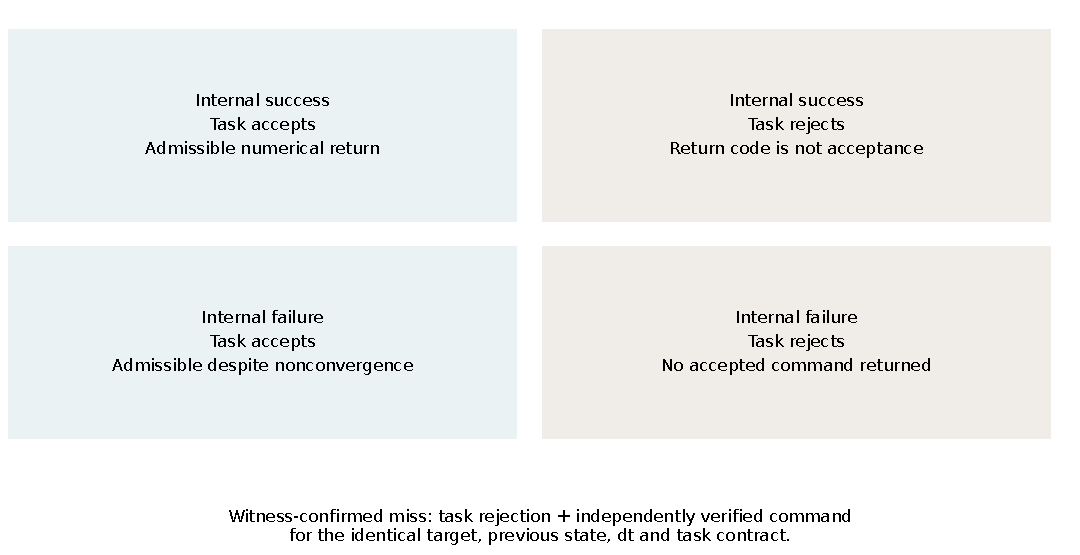
\includegraphics[width=\linewidth]{figure1_taxonomy.pdf}
\caption{Solver-internal success and task admissibility form independent outcome
axes. Deadline qualification is an additional test on accepted returns.
A witness-confirmed miss requires a legal configuration for the exact input;
a failed numerical search alone is insufficient. This schematic defines the
taxonomy and does not imply that every empirical cell is nonempty.}
\label{fig:taxonomy}
\end{figure}

\subsection{Adaptive computation as a secondary layer}

After specifying acceptance, an optional policy can allocate numerical effort.
The frozen CG-HIK case study selects among entries of a shared numerical
portfolio using query-conditioned cost predictions. Action-complete observations
measure all entries on a common input, avoiding a manually assigned difficulty
label. Predicted tail cost includes fallback work, and a shared terminal-success
target reflects the common acceptance semantics.
Reject avoids predicted futile computation; defer retains a conservative
numerical path. Neither changes the public verifier.

The empirical controls isolate direct hard entry, a geometric entry rule,
reject-only followed by hard, routing without reject, median-cost selection
and the full policy. This comparison tests whether entry ranking and failure
avoidance justify their prediction overhead. It uses frozen historical records;
the current study neither trains a policy nor adds one to the aligned native
solvers.

\section{Experimental Protocol}
\label{sec:protocol}

\subsection{Robots, numerical implementations, and common conditions}

We use the seven-joint Panda and six-joint UR5e with their original URDF geometry,
joint order and per-joint limits. The public forward-kinematics and Jacobian
backend is the repository's \texttt{URDFKinematics}; the native solver uses the
matching KDL chain. Smoke checks confirm their pose agreement and the
rotation-vector mapping. TRAC-IK is official version 2.2.0 in Speed mode with
its original internal epsilon and two native search workers.
The measured process uses the same Python 3.12.13 and NumPy 2.4.4 environment as
the authoritative Panda trajectories, on an Intel Core i7-13700K workstation.
BLAS and OpenMP thread counts are fixed to one. The Python scientific stack
supports analysis and verification \cite{virtanen2020scipy};
PyTorch and scikit-learn are used by the frozen allocation case study
\cite{paszke2019pytorch,pedregosa2011sklearn}.
No learned model is trained or changed in this study.

Six TRAC-IK point configurations are fixed: strict, position-aligned,
orientation-aligned and fully aligned at 5 ms; strict and fully aligned at
20 ms. Two DLS configurations use strict or task pose stops with the same
25-iteration cap. A fixed iteration cap is not an equal wall-time budget.
Actual return-within-budget proportions are recorded instead of assuming
that DLS is a 5 or 20 ms solver.

\subsection{Witness-feasible and inexecutable point queries}

For each robot we reuse the previously fixed set of \ev{sample.point}
witness-feasible points and \ev{sample.inexecutable} constructed inexecutable
points. The feasible families contain local, near-singular, near-limit and
hard-feasible queries, with their original proportions.
Every witness is checked under the exact input and public contract before
measurement. The inexecutable targets exceed a conservative global reach
bound obtained from URDF link translations; they are not labeled by solver
failure. Their rejection and computation are reported separately.

All settings receive identical targets, previous configurations and intervals.
Point calls do not update the previous state. TRAC-IK has three interleaved
search repeats for each input and configuration; deterministic DLS runs once.
A predetermined shuffled order interleaves the eligible settings.
The library's random search is retained, without claiming control of its
internal random seed. Raw records include native status, returned configuration,
all public checks, residuals, deadline outcome and timing components.

For both DLS point settings, an observation wrapper records actual FK evaluations
without changing numerical operations. It identifies main iterates and
line-search evaluations separately. Offline verifier replay locates the first
admissible main iterate, then counts the remaining iterations and evaluations
before the strict solver stops. Both point settings pay the same logging
instrumentation. Offline trace processing is excluded from solve latency;
no unmeasured phase-specific time saving is inferred.

\subsection{Contract-scale sensitivity}

Before any sensitivity solve, we select \ev{sample.sensitivity} fixed witnessed
queries per robot whose witnesses also pass the half-scale pose contract.
Selection uses a fixed family allocation and UID ordering, not solver outcomes.
The same inputs are evaluated at half, nominal and double position and
orientation tolerances, keeping joint limits, velocity limits, velocity allowance,
target poses, previous configurations and $\Delta t$ unchanged.
Strict TRAC-IK 5 ms, fully aligned TRAC-IK 5 ms and task-aligned DLS are the only
settings. Native bounds follow Equation~\eqref{eq:box} at every scale.
The nominal contract remains primary; a success gained by changing the public
contract is not labeled a same-contract algorithmic improvement.

\subsection{Complete continuous trajectories}

Panda's existing \ev{sample.trajectory} reference-feasible trajectories and all
of their measured runs are used unchanged. The symmetric UR5e experiment uses
\ev{sample.trajectory} new trajectories, ten each for smooth motion,
near-singular motion, joint-limit return and high curvature.
Each contains \ev{sample.frames} frames at $\Delta t=20$ ms.
The same geometry-only generator first constructs a continuous reference
joint path and then obtains targets through FK. Every reference transition
passes the public contract; identities are fixed before solver outcomes.
All trajectories are retained without success-based screening.

Every setting starts from the same initial reference configuration.
For each target it receives only that target and its own previous accepted
state. Future reference joints are stripped from the online input.
Accepted commands update the state; rejected commands hold it.
All methods still process all target frames, without restarting on the
reference branch. Four TRAC-IK configurations (strict/aligned at both budgets)
each have three full repeats; each DLS setting has one.
The new UR5e runs reuse the identical wrapper and timing scope of the prior
Panda study. No point-trace logging is enabled in either robot's trajectory
measurements.

\subsection{Measurement, statistical units, and evidence use}

Outer latency includes required input conversion, dynamic-bound construction
and setup, numerical solving, final task verification and intervening interface
costs. Initial library/chain loading and offline serialization are excluded.
Point records separately retain conversion, bounds/setup, solve, verification
and accounting remainder. Latency quantiles include failed returns; cumulative
trajectory time includes every fixed target frame.
Accepted position and orientation distributions are reported alongside success
and cost. No failure, long call or unfavorable family is deleted or winsorized.

The independent unit is the query UID for points and the complete trajectory UID
for tracking. Search repeats are averaged within each unit before paired
success-difference and mean/cumulative-cost comparisons.
We use 4,000 paired, family-stratified percentile bootstrap resamples for
95\% intervals. Frame quantiles and within-trajectory search-repeat variation
are descriptive; frames and repeated calls are not independent inferential
samples. Zero-width empirical success intervals at a ceiling do not bound
failure probability on other workloads. Family effects are reported in full
without multiple-comparison significance claims.

The point inputs have been observed in earlier mechanism work, and the Panda
trajectory outcomes predate the new supplementary experiment.
The new UR5e input identities, mappings, budgets and analysis rules were fixed
before its outcomes. This is a planned supplementary study with an authoritative
historical arm, not a claim that all evidence is a fresh formal test.
The historical allocation analysis retains its own frozen measurements and
failure semantics. All new measurements were completed and published before
manuscript reconstruction; no result triggered tuning or an additional solver.

\section{Results}
\label{sec:results}

\subsection{RQ1: How often do solver convergence and task admissibility disagree?}
\label{sec:rq1}

The first question is whether a native return flag correctly identifies commands
that satisfy the public contract. The witnessed point population separates this
question from uncertainty about whether an acceptable configuration exists.
The complete status matrix is reported in Appendix~\ref{app:matrix};
Table~\ref{tab:points} summarizes its task-level consequences. Each TRAC-IK
setting has three calls per query, whereas each DLS setting has one.

The largest observed disagreement is an internal failure that still returns an
admissible command. Strict DLS exhibits this outcome on
\ev{point.panda.dls_strict.internal_failure__task_accept} Panda queries
(\ev{dls.panda.mismatch_pct}\%) and
\ev{point.ur5e.dls_strict.internal_failure__task_accept} UR5e queries
(\ev{dls.ur5e.mismatch_pct}\%). Its internal success rates are therefore substantially
below its task-admissible rates. Accepting only a positive convergence flag would
discard these valid numerical returns. Task-aligned DLS removes this semantic
disagreement on the measured points, but the actual missed-admissible counts remain
\ev{point.panda.dls_task.miss_uid} and \ev{point.ur5e.dls_task.miss_uid}.
Changing the flag's interpretation and recovering a previously unavailable command
are different effects.

In contrast, strict and fully aligned TRAC-IK accept every witnessed nominal point
in every repeat. Their internal and task outcomes agree on this population.
Position-only alignment also retains all successes; orientation-only alignment has
\ev{point.ur5e.trac_orientation_5ms.internal_failure__task_reject} failed call on
\ev{point.ur5e.trac_orientation_5ms.miss_uid} UR5e query with a valid witness.
Thus, the component arms
recover no strict failures here. The point data do not identify a position-driven
or orientation-driven share of the later trajectory gains.
There are no internal-success/task-reject calls in the new nominal point arms.
The taxonomy accommodates that outcome without requiring every cell to be occupied.

The DLS traces explain a separate computational mismatch.
Of the \ev{dls.panda.admissible_queries} Panda and
\ev{dls.ur5e.admissible_queries} UR5e strict-DLS queries that reach an admissible
main iterate, \ev{dls.panda.positive_excess_queries} and
\ev{dls.ur5e.positive_excess_queries} continue iterating.
The median is \ev{dls.panda.median_excess_iterations} excess iteration and the
P95 is \ev{dls.panda.p95_excess_iterations} for both robots
(Appendix~\ref{app:trace}). These are directly observed excess iterations after
task admissibility, not an inference from separate runtimes.
TRAC-IK does not expose a comparable trace.

All constructed inexecutable points are rejected by every setting, with no false
acceptance. Independently replaying the point and trajectory returns finds
\ev{verification.violations} accepted contract violations.
The observed disagreement is therefore concentrated in strict DLS's interpretation
of otherwise admissible returns; the next question is whether native tolerance
alignment reduces computation under unchanged public acceptance.

\begin{table}[tb]
\centering\small
\setlength{\tabcolsep}{3pt}
\caption{Witness-feasible point queries, \ev{sample.point} independent queries per
robot. Internal and verified columns are percentages. Miss is the number of UIDs
with at least one missed-admissible call. TRAC-IK has three within-query repeats;
DLS has one. All latency columns are milliseconds and include the final verifier.
DLS point timings include the same trace instrumentation in both settings.}
\label{tab:points}
\begin{tabular}{llrrrrrrr}\toprule
Robot & Setting & Internal & Verified & Miss & Mean & P50 & P95 & P99\\\midrule
Panda & TRAC strict 5 ms & 100.00 & 100.00 & 0 & 0.236 & 0.211 & 0.367 & 0.487 \\
Panda & TRAC position 5 ms & 100.00 & 100.00 & 0 & 0.241 & 0.211 & 0.379 & 0.681 \\
Panda & TRAC orientation 5 ms & 100.00 & 100.00 & 0 & 0.247 & 0.210 & 0.382 & 0.799 \\
Panda & TRAC aligned 5 ms & 100.00 & 100.00 & 0 & 0.221 & 0.199 & 0.332 & 0.478 \\
Panda & TRAC strict 20 ms & 100.00 & 100.00 & 0 & 0.236 & 0.211 & 0.362 & 0.485 \\
Panda & TRAC aligned 20 ms & 100.00 & 100.00 & 0 & 0.220 & 0.199 & 0.331 & 0.467 \\
Panda & DLS strict & 77.56 & 99.48 & 13 & 3.015 & 1.038 & 8.944 & 9.230 \\
Panda & DLS aligned & 99.48 & 99.48 & 13 & 0.762 & 0.625 & 1.042 & 4.479 \\
UR5e & TRAC strict 5 ms & 100.00 & 100.00 & 0 & 0.218 & 0.201 & 0.318 & 0.409 \\
UR5e & TRAC position 5 ms & 100.00 & 100.00 & 0 & 0.216 & 0.199 & 0.317 & 0.414 \\
UR5e & TRAC orientation 5 ms & 99.99 & 99.99 & 1 & 0.219 & 0.200 & 0.324 & 0.445 \\
UR5e & TRAC aligned 5 ms & 100.00 & 100.00 & 0 & 0.209 & 0.191 & 0.312 & 0.415 \\
UR5e & TRAC strict 20 ms & 100.00 & 100.00 & 0 & 0.222 & 0.200 & 0.320 & 0.424 \\
UR5e & TRAC aligned 20 ms & 100.00 & 100.00 & 0 & 0.210 & 0.192 & 0.313 & 0.410 \\
UR5e & DLS strict & 78.72 & 99.96 & 1 & 2.757 & 1.185 & 8.113 & 8.427 \\
UR5e & DLS aligned & 99.96 & 99.96 & 1 & 0.656 & 0.578 & 0.926 & 1.458 \\
\bottomrule

\end{tabular}
\end{table}

\subsection{RQ2: Does contract alignment improve task-level success and computation?}
\label{sec:rq2}

With acceptance held fixed, does using the available pose tolerance reduce work,
and does any gain persist across contracts and solver budgets?
Figure~\ref{fig:points} shows all prespecified point settings.
On the nominal witnessed points, fully aligned TRAC-IK at 5 ms reduces mean
whole-call time by
\ev{point.panda.trac_task_5ms.contrast.saving_pct}\% on Panda and
\ev{point.ur5e.trac_task_5ms.contrast.saving_pct}\% on UR5e, while preserving complete
success. The paired mean-cost ratios are
\ev{point.panda.trac_task_5ms.contrast.time_ratio} and
\ev{point.ur5e.trac_task_5ms.contrast.time_ratio}, respectively
(brackets denote 95\% intervals). These are modest interface-level savings on a
population that strict TRAC-IK already solves reliably.

Partial alignment has no uniform cost advantage. On Panda, position-only and
orientation-only cost ratios are
\ev{point.panda.trac_position_5ms.contrast.time_ratio} and
\ev{point.panda.trac_orientation_5ms.contrast.time_ratio}.
The corresponding UR5e ratios are
\ev{point.ur5e.trac_position_5ms.contrast.time_ratio} and
\ev{point.ur5e.trac_orientation_5ms.contrast.time_ratio}.
Tolerance dimensions interact with numerical search, so the effects of the
component arms need not add to the fully aligned effect.
Increasing strict TRAC-IK's budget to 20 ms adds no point successes.
Constructed inexecutable requests still consume approximately the search budget
under either mapping; their cost is reported separately in the source tables.

Task-aligned DLS preserves the same point-level acceptance sets while reducing
mean time by \ev{point.panda.dls_task.contrast.saving_pct}\% and
\ev{point.ur5e.dls_task.contrast.saving_pct}\%.
P95 falls from \ev{point.panda.dls_strict.p95} to
\ev{point.panda.dls_task.p95} ms on Panda and from
\ev{point.ur5e.dls_strict.p95} to \ev{point.ur5e.dls_task.p95} ms on UR5e.
The direct trace evidence supports attributing this reduction to earlier stopping,
within the instrumentation scope of these measurements. Absolute DLS and native
TRAC-IK times also reflect different implementations and are not equal-time-budget
comparisons.

The saved work accompanies larger legal errors. For fully aligned TRAC-IK at
5 ms, accepted position P95 rises from
\ev{point.panda.trac_strict_5ms.position_p95} to
\ev{point.panda.trac_task_5ms.position_p95} mm on Panda and from
\ev{point.ur5e.trac_strict_5ms.position_p95} to
\ev{point.ur5e.trac_task_5ms.position_p95} mm on UR5e.
Accepted orientation P95 becomes
\ev{point.panda.trac_task_5ms.orientation_p95}$^\circ$ and
\ev{point.ur5e.trac_task_5ms.orientation_p95}$^\circ$.
The full error distributions, including maxima and DLS returns, accompany the
source tables. These errors spend an existing task allowance; the final nominal
limits have not changed.

\begin{figure}[tb]
\centering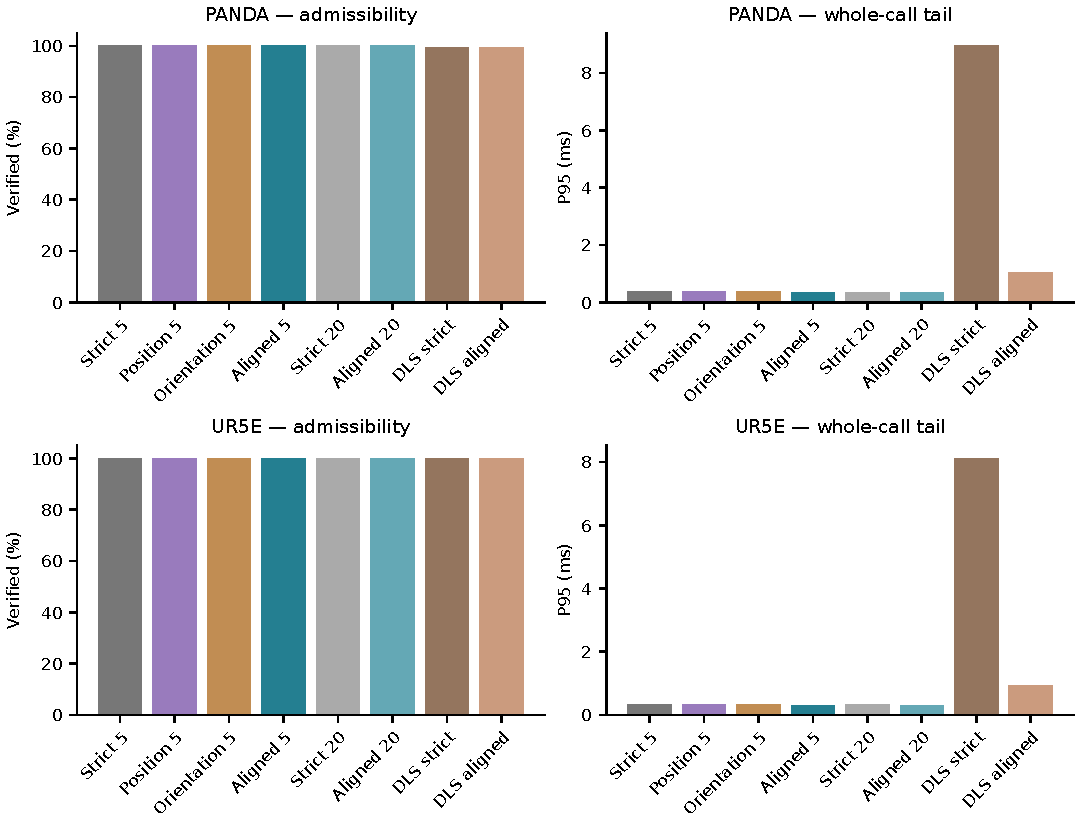
\includegraphics[width=\linewidth]{figure2_point_alignment.pdf}
\caption{Nominal witnessed points for both robots. Verified success and whole-call
P95 are shown separately for every prescribed setting. The near-ceiling success
bars should be read with the exact counts in Table~\ref{tab:points}.
The numbers 5 and 20 label TRAC-IK search budgets in milliseconds; DLS uses a fixed
iteration cap. Bars are descriptive call summaries, not independent-call inference.}
\label{fig:points}
\end{figure}

\begin{figure}[tb]
\centering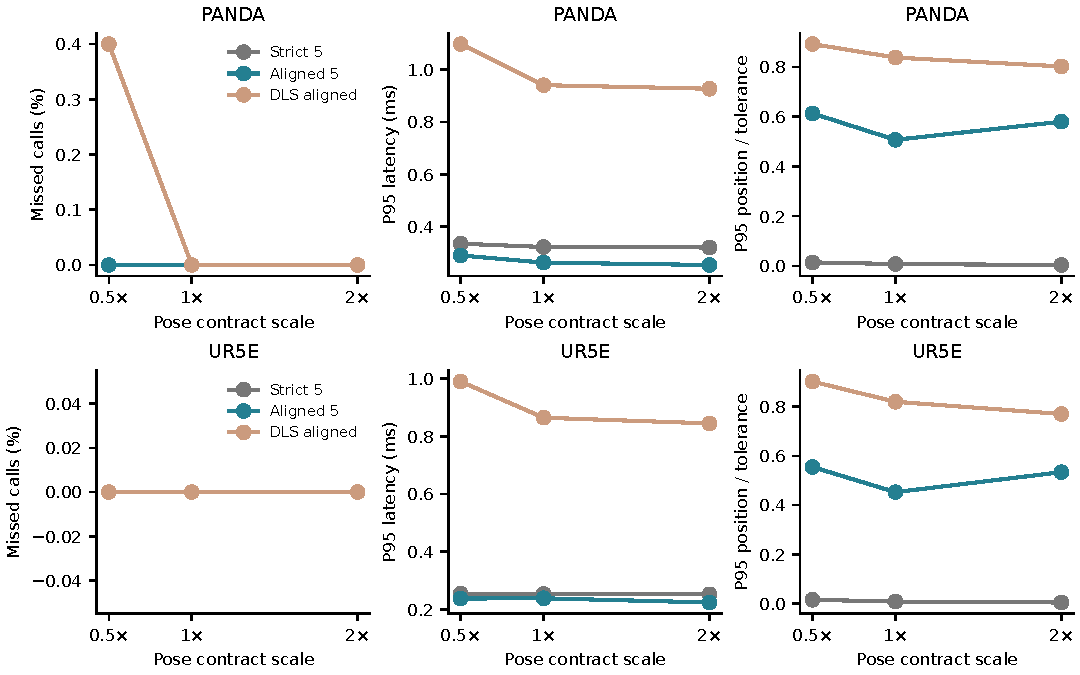
\includegraphics[width=\linewidth]{figure3_contract_sensitivity.pdf}
\caption{Contract sensitivity on the same \ev{sample.sensitivity} witnessed queries
per robot at every scale. Only the two pose tolerances change. Missed-call rates,
whole-call P95, and accepted position P95 divided by the applicable tolerance are
shown. Overlapping zero-miss curves indicate complete observed success; they do
not establish zero population failure probability. Orientation distributions are
included in the accompanying source data.}
\label{fig:scales}
\end{figure}

Across the fixed contract scales, strict and fully aligned TRAC-IK remain fully
successful (Figure~\ref{fig:scales}). Panda task-aligned DLS misses
\ev{sensitivity.panda.dls_task.0.5.miss_uid} queries at
the half-scale contract and none at nominal or double scale; UR5e misses none.
Its mean times decrease as the permitted pose sets expand.
Fully aligned TRAC-IK also generally obtains a larger relative mean-cost advantage
at larger scales, although individual quantiles are not strictly monotonic.
The scale study therefore supports a computational interpretation, not a broad
claim of tolerance-dependent recovery for TRAC-IK on these points.
Alignment reduces work under a fixed nominal contract in both implementations,
but whether earlier accepted commands sustain a continuous trajectory requires
a closed-loop test.

\subsection{RQ3: Does the effect persist in trajectories, and when is adaptive computation useful?}
\label{sec:rq3}

A faster admissible point return is useful online only if the resulting sequence
continues to meet the contract. We therefore compare complete trajectories with
each setting feeding back its own last accepted command. Table~\ref{tab:trajectories}
and Figure~\ref{fig:trajectories} retain every target frame and every planned
search repeat.

At 5 ms, Panda TRAC-IK completion increases from
\ev{trajectory.panda.trac_strict_5ms.completion} to
\ev{trajectory.panda.trac_task_5ms.completion} out of
\ev{sample.trajectory} per sweep.
UR5e increases from \ev{trajectory.ur5e.trac_strict_5ms.completion} to
\ev{trajectory.ur5e.trac_task_5ms.completion}.
No strict-completed UID is lost. The paired completion-rate differences are
\ev{trajectory.panda.trac_task_5ms.contrast.success_pp} percentage points for Panda
and \ev{trajectory.ur5e.trac_task_5ms.contrast.success_pp} for UR5e.
Cumulative solver time decreases by
\ev{trajectory.panda.trac_task_5ms.contrast.saving_pct}\% and
\ev{trajectory.ur5e.trac_task_5ms.contrast.saving_pct}\%;
paired cost ratios are \ev{trajectory.panda.trac_task_5ms.contrast.time_ratio} and
\ev{trajectory.ur5e.trac_task_5ms.contrast.time_ratio}.
The intervals reflect independent trajectory variation, not thousands of
independent frames.

Larger search budgets do not substitute for the mapping.
Strict TRAC-IK at 20 ms completes the same number of trajectories as strict 5 ms
on both robots, while spending more time on unsuccessful requests.
Aligned 20 ms sometimes completes more Panda paths than aligned 5 ms, but raises
cumulative time; UR5e completion is unchanged.
Whole-trajectory deadline success is separately listed in
Table~\ref{tab:trajectories}. Occasional late frames make it differ from geometric
completion even when the nominal sampling interval is 20 ms.

The family analysis localizes the gains rather than hiding them in a total.
Panda's 5 ms recovery is confined to near-singular paths.
UR5e gains \ev{family.ur5e.smooth.gained} smooth and
\ev{family.ur5e.high_curvature.gained} high-curvature path, while its near-singular
completion remains unchanged. Joint-limit-return UR5e time changes little, and
Panda high-curvature time does not improve.
Figure~\ref{fig:families} and Appendix~\ref{app:family} include every family.

\begin{table}[tb]
\centering\small\setlength{\tabcolsep}{3pt}
\caption{Complete online trajectories. Each robot has \ev{sample.trajectory}
independent paths with \ev{sample.frames} targets each. Complete and deadline columns
give counts per planned sweep; the latter requires every frame to be admissible
and returned within 20 ms. Frame is the verified percentage. Time is cumulative
seconds per full sweep, averaged over the three TRAC-IK sweeps. Latency quantiles
are in milliseconds. Panda measurements are the unchanged authoritative prior runs.}
\label{tab:trajectories}
\begin{tabular}{llrrrrrrr}\toprule
Robot & Setting & Complete & Deadline & Frame & Time & P50 & P95 & P99\\\midrule
Panda & TRAC strict 5 ms & 34/34/34 & 34/34/33 & 93.98 & 3.187 & 0.190 & 5.249 & 5.434 \\
Panda & TRAC aligned 5 ms & 36/37/37 & 36/36/37 & 97.28 & 2.150 & 0.179 & 0.484 & 5.305 \\
Panda & TRAC strict 20 ms & 34/34/34 & 34/34/34 & 93.99 & 8.654 & 0.192 & 20.352 & 20.559 \\
Panda & TRAC aligned 20 ms & 37/37/38 & 37/37/38 & 98.16 & 3.600 & 0.180 & 0.462 & 20.392 \\
Panda & DLS strict & 37 & 37 & 96.80 & 14.255 & 0.943 & 9.119 & 10.624 \\
Panda & DLS aligned & 37 & 37 & 96.80 & 4.814 & 0.550 & 1.451 & 6.830 \\
UR5e & TRAC strict 5 ms & 37/37/37 & 37/37/37 & 96.82 & 2.032 & 0.169 & 0.300 & 5.256 \\
UR5e & TRAC aligned 5 ms & 39/39/39 & 39/39/39 & 99.57 & 1.167 & 0.161 & 0.223 & 0.405 \\
UR5e & TRAC strict 20 ms & 37/37/37 & 37/36/37 & 96.82 & 4.932 & 0.169 & 0.303 & 20.357 \\
UR5e & TRAC aligned 20 ms & 39/39/39 & 39/39/38 & 99.58 & 1.568 & 0.161 & 0.229 & 0.412 \\
UR5e & DLS strict & 35 & 35 & 95.32 & 16.965 & 0.816 & 7.813 & 7.955 \\
UR5e & DLS aligned & 28 & 28 & 88.37 & 6.586 & 0.495 & 5.066 & 7.769 \\
\bottomrule

\end{tabular}
\end{table}

\begin{figure}[p]
\centering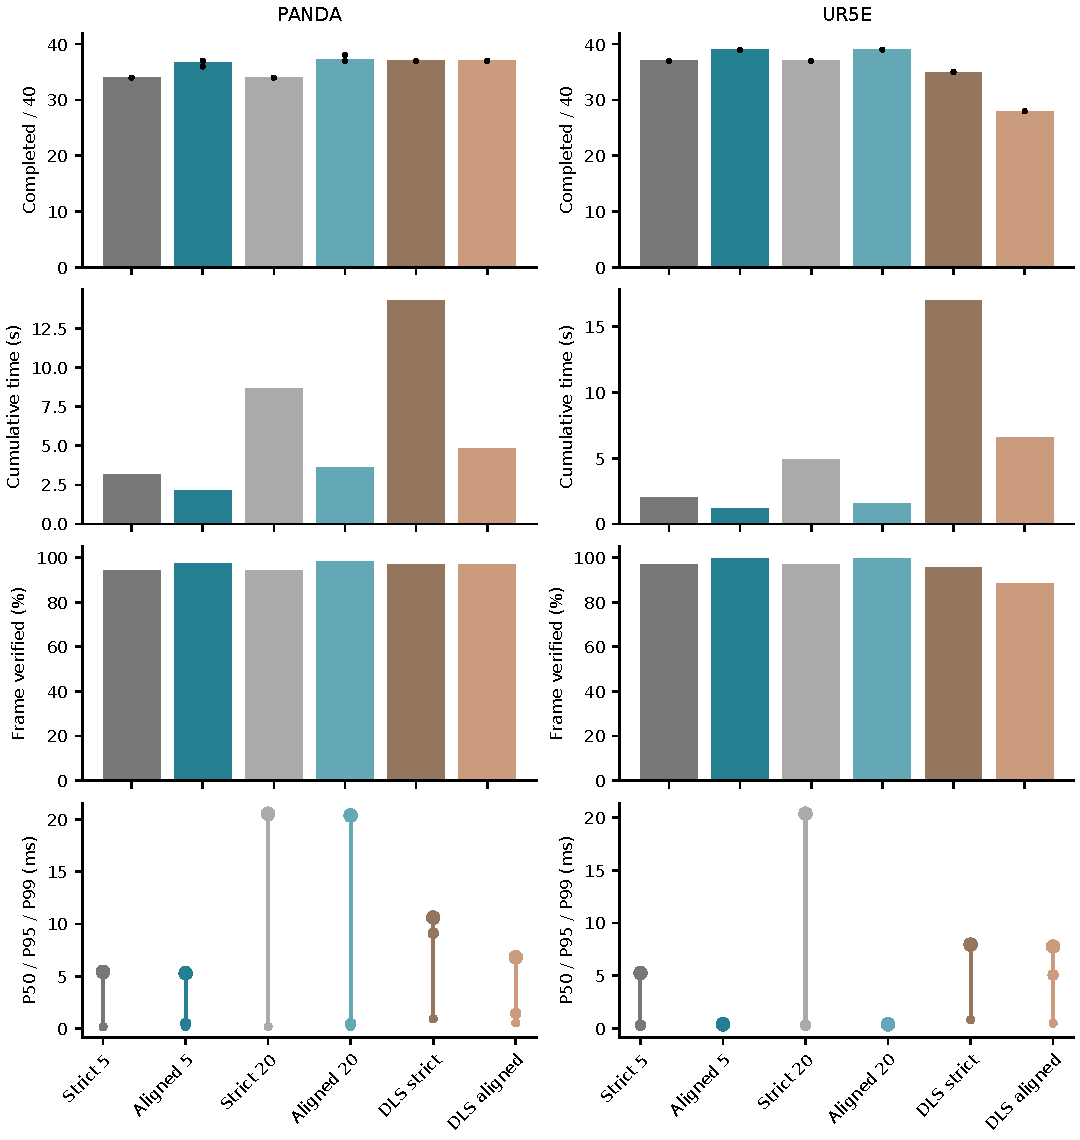
\includegraphics[width=.96\linewidth]{figure4_trajectories.pdf}
\caption{Continuous online operation. Columns separate robots; rows report
geometric completion, cumulative cost, frame admissibility and latency quantiles.
Dots on completion bars show the planned search repeats. In the bottom row,
increasing marker sizes denote P50, P95 and P99; connecting segments only group
the three quantiles of one setting. All fixed target frames contribute to cost.
UR5e's lower DLS-aligned completion is retained alongside its lower cost.}
\label{fig:trajectories}
\end{figure}

\begin{figure}[tb]
\centering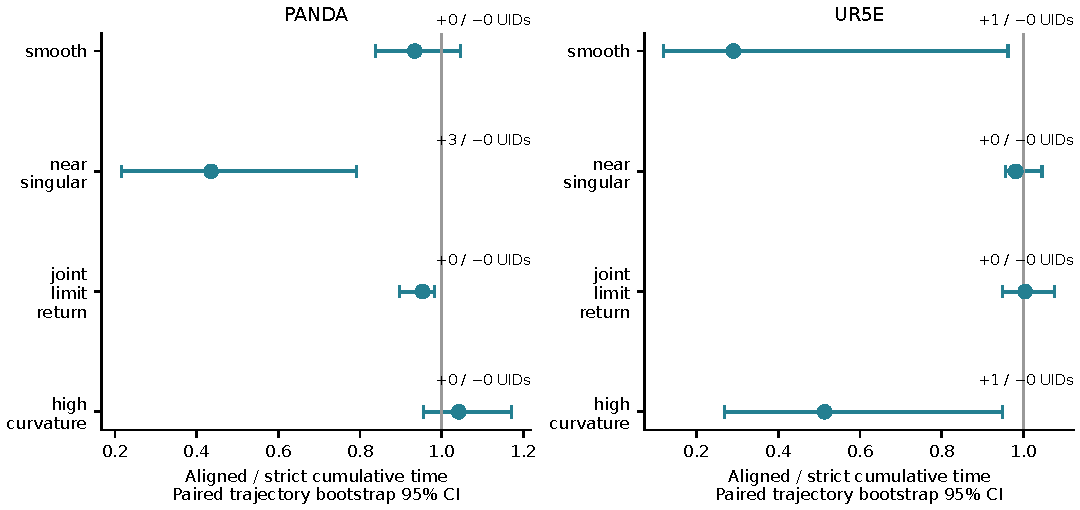
\includegraphics[width=\linewidth]{figure5_family_effects.pdf}
\caption{Fully aligned versus strict TRAC-IK at 5 ms, by trajectory family.
Intervals resample paired trajectory UIDs within the stated family.
Annotations count UIDs with increased/decreased completion fractions across repeats,
not independent new paths; Panda's gains include a partial search-repeat recovery.
The reference line denotes unchanged cumulative cost.}
\label{fig:families}
\end{figure}

DLS exposes an important boundary. On Panda, both stopping rules complete
\ev{trajectory.panda.dls_task.completion} paths, and task alignment reduces cumulative
time by \ev{trajectory.panda.dls_task.contrast.saving_pct}\%.
On UR5e, completion falls from \ev{trajectory.ur5e.dls_strict.completion} to
\ev{trajectory.ur5e.dls_task.completion}, losing
\ev{trajectory.ur5e.dls_task.contrast.lost} strict-completed paths despite saving
\ev{trajectory.ur5e.dls_task.contrast.saving_pct}\% of cumulative computation.
The completion difference is
\ev{trajectory.ur5e.dls_task.contrast.success_pp} percentage points.
The losses span smooth, near-singular and joint-limit-return families.
Both settings still submit only admissible commands. Earlier stopping therefore
changes more than time spent on the current query: it changes the configuration
presented to subsequent queries. These trajectories do not isolate the cause of
each failure or establish infeasibility from the failed setting's state.

\paragraph{The residual role of computation allocation.}
The frozen CG-HIK case study asks whether additional entry selection compensates
for its own overhead. Table~\ref{tab:allocation} uses historical paired point
measurements, not newly routed calls to the aligned solvers.
On witnessed points, full CG-HIK matches direct hard-entry success but increases
mean time by \ev{allocation.panda.full_hard.time_increase_pct}\% on Panda and
\ev{allocation.ur5e.full_hard.time_increase_pct}\% on UR5e.
Routing-only is also slower, and a geometric entry rule is close to the full
policy. Selecting by predicted P95 rather than P50 reduces function evaluations
by \ev{allocation.panda.p95_p50.fev_reduction_pct}\% and
\ev{allocation.ur5e.p95_p50.fev_reduction_pct}\%, but its P95 and P99 ratio
intervals include unity on both robots.

Post-hoc decomposition of the original transition-rich workload assigns
\ev{allocation.panda.joint_failure_share}\% and
\ev{allocation.ur5e.joint_failure_share}\% of net time savings to paths neither
method completed. A share above one hundred percent means that savings in that
group offset additional cost elsewhere. Independently witnessed reference paths
likewise provide no universal successful-tracking advantage for learned routing.
Reject-only controls show that avoiding unsuccessful numerical work is useful
on failure-heavy requests. The historical external TRAC-IK comparison is much
faster than this learned/numerical portfolio; its documented floating-point
endpoint issue remains an implementation caveat, not a newly attributed
tolerance-alignment benefit.

Taken together, continuous trajectories support the aligned TRAC-IK interface on
both tested robots while revealing a DLS stopping-rule trade-off that points alone
miss. The allocation evidence favors paying for a secondary decision layer only
when the remaining unsuccessful-solve cost is large enough to justify it.

\begin{table}[tb]
\centering\small
\caption{Secondary allocation case study on the same historical witnessed point
population. Ratios compare the named policies; brackets are paired query-level
95\% intervals. The success difference is in percentage points.
Geometry and reject-only controls retain the same reject/defer predictor.
These are not new measurements of a router added to aligned TRAC-IK or DLS.}
\label{tab:allocation}
\begin{tabular}{llrrr}\toprule
Robot & Contrast & Mean time ratio & FEV ratio & Success diff.\\\midrule
panda & Full / hard & 1.033 [1.029, 1.038] & 1.001 [1.001, 1.002] & 0.00 \\
panda & Routing-only / hard & 1.033 [1.030, 1.038] & 1.001 [1.001, 1.002] & 0.00 \\
panda & Full / geometry & 1.001 [1.000, 1.002] & 1.001 [1.000, 1.001] & 0.00 \\
panda & Full / reject-only & 1.000 [0.998, 1.001] & 1.001 [1.001, 1.002] & 0.00 \\
panda & P95 / P50 selection & 0.998 [0.997, 1.000] & 0.994 [0.992, 0.996] & 0.00 \\
ur5e & Full / hard & 1.293 [1.286, 1.300] & 1.000 [1.000, 1.001] & 0.00 \\
ur5e & Routing-only / hard & 1.294 [1.286, 1.300] & 1.000 [1.000, 1.001] & 0.00 \\
ur5e & Full / geometry & 1.002 [0.998, 1.005] & 0.999 [0.996, 1.000] & 0.00 \\
ur5e & Full / reject-only & 1.002 [0.998, 1.005] & 1.000 [1.000, 1.001] & 0.00 \\
ur5e & P95 / P50 selection & 0.998 [0.994, 1.002] & 0.981 [0.974, 0.989] & 0.00 \\
\bottomrule

\end{tabular}
\end{table}

\section{Discussion}
\label{sec:discussion}

\subsection{A return code answers a different question from a task verifier}

A native convergence flag describes whether a numerical procedure met its
configured conditions. The public verifier describes whether its returned
configuration meets the command contract. Strict DLS demonstrates the practical
difference: many negative flags accompany legal returns, and its observed
iteration traces show substantial work after admissibility.
TRAC-IK's agreement on the witnessed point population is equally informative.
An explicit taxonomy helps identify when disagreement matters; it does not
require disagreement to be common in every solver.

Witnesses strengthen failure interpretation only when they refer to an identical
input. The point dataset supplies that comparison directly.
Reference paths in the trajectory study supply a weaker existence statement:
they verify the reference sequence, not every state visited by another solver.
Accordingly, improved closed-loop completion is evidence about the interface
and its induced trajectory, while individual failures remain numerical outcomes
unless an exact-input witness has been saved.

\subsection{Alignment can remove work, but earlier acceptance changes feedback}

The DLS trace supplies direct evidence for excess iterations after task
admissibility. Allowing termination at the public pose threshold reduces that
work on both point populations. Fully aligned TRAC-IK has smaller point-level
cost benefits and larger continuous-trajectory benefits. A longer strict search
budget does not recover the same completions, which argues against attributing
the trajectory difference solely to too little wall time. Because its internal
search path is not observed, the TRAC-IK measurements establish outcomes rather
than a count of unnecessary internal iterations.

The UR5e DLS result limits the interpretation of earlier stopping.
An admissible set can contain configurations with different subsequent tracking
behavior. Stopping at its first reached point changes the feedback state and
may preserve less useful pose accuracy or joint-space geometry for the next
target. The present comparison changes those quantities together; it does not
identify either as the sole cause. Thus, contract-aware acceptance is a sound
interface requirement, but choosing the earliest admissible iterate is not
guaranteed to preserve whole-trajectory completion. The difference between the
two robots is part of the finding: contract mismatch and the benefit of its
correction are robot-, solver- and workload-dependent.

\subsection{Using a task allowance is not loosening the final task}

The strict/aligned comparisons retain identical public position, orientation,
joint and rate tests. Task-aligned returns have larger residuals because they
use an allowance already present in that contract. Reporting those distributions
makes the precision--computation trade-off visible without treating all accepted
commands as equally accurate.
For an application that requires tighter pose accuracy, the correct response
is a tighter public contract and a corresponding native mapping, not an
undocumented strict threshold inside one baseline.

The sensitivity study makes that distinction explicit. It changes the public
pose contract in separate, prespecified arms while preserving the same witnessed
inputs and motion limits. Increasing the permitted pose set generally reduces
aligned computation, but the nominal point TRAC-IK success ceiling leaves no
recovery trend to estimate. Moreover, the inscribed native box may exclude
legal norm-ball residuals. Conservativeness protects the interpretation of
native bounds; it does not make the two admissible sets equivalent or ensure
that the solver finds all legal commands.

\subsection{Allocation should be judged after the numerical interface}

The historical allocation study shows why aggregate speed alone can mislead
solver-design decisions. Avoiding futile fallback work can save considerable
time even when successful paths do not become faster. A learned entry policy
can also reduce numerical evaluations yet lose that saving to inference and
interface overhead. These are useful distinctions for engineering a service
that processes both feasible and failure-heavy requests.

For the measured portfolio, complex routing does not generally accelerate
successful IK, and simple entry controls are competitive. Reject remains useful
when unsuccessful numerical work is expensive. The current native comparison
does not directly measure a router added to an aligned solver, so its marginal
value in that setting is an empirical boundary rather than a new measured
speedup. The supported ordering is nevertheless concrete: first establish a
common command contract, configure the numerical interface to use it, and then
compare the remaining failed-request cost with the full overhead of any
adaptive decision. Better configuration of a mature solver is an engineering
result, not a reason to rename that solver as a new algorithm.

\section{Limitations}
\label{sec:limitations}

The study uses exact software kinematics on two manipulators. It excludes
collision checking, dynamics, contact, torque limits, calibration uncertainty
and physical controller behavior. Geometric admissibility under the stated
contract is not physical safety certification. The 20 ms deadline is an
evaluation endpoint; nominal sampling at that interval does not establish
hard real-time control.

TRAC-IK and the existing Adaptive DLS are the only newly measured solvers.
Their native acceptance regions differ, with the component box conservatively
approximating a norm ball. Search budgets and iteration caps are not equivalent
resources. Absolute latency depends on hardware, native/Python implementation,
threading, operating-system scheduling and the shared workstation.
Both DLS point settings include trace logging, whereas trajectories use the
same uninstrumented wrapper across robots.

The supplementary point workload is fixed and previously observed, and its
TRAC-IK success ceiling limits recovery analysis. Panda's authoritative
trajectories were measured earlier than the symmetric UR5e runs.
The paired intervals quantify variation within the sampled families, not
coverage of all online IK tasks. A reference-feasible path does not guarantee
a legal continuation from every method-specific state.
Finally, the allocation boundary uses historical controls rather than a new
factorial experiment adding a router to each aligned solver. The conclusions
therefore distinguish directly measured alignment effects from the engineering
judgment about when an additional decision layer is worth its cost.

\section{Conclusions}
\label{sec:conclusions}

Solver convergence is not command admissibility.
A common task contract separates native convergence, legal command generation
and deadline-qualified success, and provides a basis for configuring existing
solver interfaces. In this study, task-aligned TRAC-IK preserves point success,
improves complete tracking on both robots and reduces cumulative trajectory
computation under the same final acceptance conditions. DLS exposes frequent
internal-failure/admissible-return disagreement and excess iterations, but its
UR5e completion loss shows that earlier local acceptance is not a universal
closed-loop improvement. The frozen allocation case study further places most
aggregate benefit in failure handling rather than broadly faster successful
entry selection.

The resulting design principle is to align the solver with the task contract
before introducing adaptive computation. Any subsequent allocation layer should
earn its overhead from the residual workload, with success, precision and
complete-trajectory behavior reported alongside time.

\section*{Data and code availability}

The implementation, fixed protocol, input identities, raw returned configurations,
timing records, aggregate tables and verified witness indices are available in
the public repository \url{https://github.com/dingzhen60027/CG-HIK}, branch
\texttt{codex/hierarchical-v5}. The paper's evidence snapshot identifies the
frozen measurement commit and file hashes. Manuscript numbers and figures are
generated from those records without solving new queries. Historical evidence
and the previous manuscript are retained separately. The repository supports
inspection of the reported software benchmark; it is not a hardware deployment
package.

\appendix
\section{Complete nominal point outcome matrix}
\label{app:matrix}

Table~\ref{tab:matrix} gives raw call counts for the witnessed nominal population.
The independent sample size remains \ev{sample.point} query UIDs per robot.
Every internal-failure/task-reject entry in this population has a saved legal
witness under the identical input. Counts across search repeats do not represent
additional independent queries.

\begin{table}[htbp]
\centering\small
\caption{Native/task outcome matrix for witnessed nominal points.
$I$ is native success and $A$ is task acceptance. Three TRAC-IK calls and one
DLS call per UID are retained; counts are not pooled into a larger statistical
sample. Constructed inexecutable points are reported separately in source data.}
\label{tab:matrix}
\begin{tabular}{llrrrr}\toprule
Robot & Setting & $I{=}1,A{=}1$ & $I{=}1,A{=}0$ & $I{=}0,A{=}1$ & $I{=}0,A{=}0$\\\midrule
panda & TRAC position 5 ms & 7500 & 0 & 0 & 0 \\
panda & DLS strict & 1939 & 0 & 548 & 13 \\
panda & TRAC aligned 5 ms & 7500 & 0 & 0 & 0 \\
panda & TRAC strict 5 ms & 7500 & 0 & 0 & 0 \\
panda & TRAC aligned 20 ms & 7500 & 0 & 0 & 0 \\
panda & TRAC strict 20 ms & 7500 & 0 & 0 & 0 \\
panda & TRAC orientation 5 ms & 7500 & 0 & 0 & 0 \\
panda & DLS aligned & 2487 & 0 & 0 & 13 \\
ur5e & TRAC position 5 ms & 7500 & 0 & 0 & 0 \\
ur5e & DLS strict & 1968 & 0 & 531 & 1 \\
ur5e & TRAC aligned 5 ms & 7500 & 0 & 0 & 0 \\
ur5e & TRAC strict 5 ms & 7500 & 0 & 0 & 0 \\
ur5e & TRAC aligned 20 ms & 7500 & 0 & 0 & 0 \\
ur5e & TRAC strict 20 ms & 7500 & 0 & 0 & 0 \\
ur5e & TRAC orientation 5 ms & 7499 & 0 & 0 & 1 \\
ur5e & DLS aligned & 2499 & 0 & 0 & 1 \\
\bottomrule

\end{tabular}
\end{table}

\section{Directly observed DLS excess iterations}
\label{app:trace}

The observation wrapper records the unchanged solver's FK calls and identifies
main iterates by their call site. A complete residual/evaluation trace remains
available for every strict point query, including those that never produce an
admissible iterate. Figure~\ref{fig:excess} conditions only the excess-iteration
quantity on its being defined. The full population is retained in the source
table; a query without an admissible iterate is not assigned zero excess work.
No comparable unobserved TRAC-IK iteration quantity is inferred.

\begin{figure}[htbp]
\centering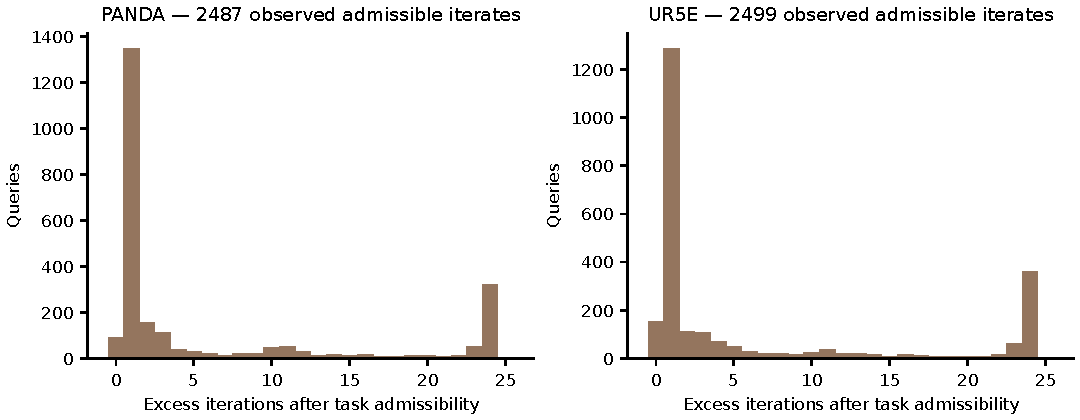
\includegraphics[width=\linewidth]{supplement_dls_excess_iterations.pdf}
\caption{Excess iterations after task admissibility in strict DLS.
Each included query contributes its stopping iteration minus its first admissible
main-iterate index. Panel titles count queries with such an iterate, not
independent iteration samples. Remaining queries are retained with undefined
excess values in source data. Phase-specific extra time is not estimated.}
\label{fig:excess}
\end{figure}

\section{Complete family-level trajectory effects}
\label{app:family}

\begin{table}[htbp]
\centering\small\setlength{\tabcolsep}{4pt}
\caption{Fully aligned/strict TRAC-IK at 5 ms for all trajectory families.
Each family contains ten independent paths. Completion lists correspond to
three complete search repeats; intervals use paired trajectory resampling.
Gained/lost counts compare per-UID completion fractions.}
\label{tab:family}
\begin{tabular}{llrrrl}\toprule
Robot & Family & Strict & Aligned & Cost ratio [95\% CI] & Gain/loss\\\midrule
panda & high curvature & 10/10/10 & 10/10/10 & 1.042 [0.955, 1.170] & 0/0 \\
panda & joint limit return & 9/9/9 & 9/9/9 & 0.953 [0.897, 0.982] & 0/0 \\
panda & near singular & 5/5/5 & 7/8/8 & 0.435 [0.215, 0.792] & 3/0 \\
panda & smooth & 10/10/10 & 10/10/10 & 0.934 [0.837, 1.047] & 0/0 \\
ur5e & high curvature & 9/9/9 & 10/10/10 & 0.514 [0.268, 0.948] & 1/0 \\
ur5e & joint limit return & 10/10/10 & 10/10/10 & 1.004 [0.949, 1.075] & 0/0 \\
ur5e & near singular & 9/9/9 & 9/9/9 & 0.981 [0.955, 1.045] & 0/0 \\
ur5e & smooth & 9/9/9 & 10/10/10 & 0.290 [0.120, 0.962] & 1/0 \\
\bottomrule

\end{tabular}
\end{table}

The distributed CSV/JSON tables additionally provide per-trajectory cumulative
mean, median and P95, completion UID sets, accepted-error distributions,
first-failure inputs and reasons, and repeated-search variability.
All full trajectories and returned configurations can be inspected through
the witness and run indices. No conclusion requires selecting only the
successful trajectories.

\FloatBarrier
\bibliographystyle{unsrtnat}
\bibliography{references}

\end{document}
